%all chapter has been typed

%done till prob 4.20 (p179) and then after MISSING PAGES
%from  sec 4.4.1 spin 1/2 page 185 till start of prob 4.33



\باب{تین ابعادی کوانٹم میکانیات}\شناخت{باب_تین_ابعادی_کوانٹم_میکانیات}
\حصہ{کروی محدد میں مساوات شروڈنگر}
تین ابعاد تک توسیع  باآسانی کی جا سکتی ہے۔ مساوات شروڈنگر درج ذیل کہتی ہے
\begin{align}
i\hslash\frac{\dif{\Psi}}{\dif{t}}=H\Psi;
\end{align}
معیاری طریقہ کار کے اطلاق \عددی{x}  کے ساتھ ساتھ \عددی{y} اور \عددی{z} پر  کر کے:
\begin{align}\label{مساوات_تین_ابعاد_عاملین_الف}
 p_{x}\to \frac{\hslash}{i}\frac{\partial}{\partial{x}},\quad p_{y}\to \frac{\hslash}{i}\frac{\partial}{\partial{y}},\quad p_{z}\to \frac{\hslash}{i}\frac{\partial}{\partial{z}} 
\end{align}
ہیملٹنی\حاشیہد{جہاں کلاسیکی مشہود اور عامل میں فرق کرنا دشوار ہو، وہاں میں عامل پر "ٹوپی" کا نشان بناتا ہوں۔ اس باب میں ایسا کوئی موقع نہیں پایا جاتا جہاں ان کی پہچان مشکل ہو لہٰذا یہاں سے عاملین پر "ٹوپی" کا نشان نہیں ڈالا جائے گا۔} عامل \عددی{H} کو کلاسیکی توانائی
\begin{align*}
\frac{1}{2}mv^{2}+V=\frac{1}{2m}(p_{x}^{2}+p_{y}^{2}+p_{z}^{2})+V
\end{align*}
سے حاصل کیا جاتا ہے۔ مساوات \حوالہ{مساوات_تین_ابعاد_عاملین_الف} کو مختصراً درج ذیل لکھا  جا سکتا ہے۔
\begin{align}
p\to \frac{\hslash}{i}\nabla
\end{align}
یوں درج ذیل ہو گا
\begin{align}
i\hslash\frac{\partial{\Psi}}{\partial{t}}=-\frac{\hslash^{2}}{2m}\nabla^{2}\Psi+V\Psi
\end{align}
جہاں
\begin{align}
\nabla^{2}\equiv \frac{\partial^{\,2}}{\partial{x^2}}+\frac{\partial^{\,2}}{\partial{y^2}}+\frac{\partial^{\,2}}{\partial{z^2}} 
\end{align}
کارتیسی محدد میں \اصطلاح{لاپلاسی}\فرہنگ{لاپلاسی}\حاشیہب{Laplacian}\فرہنگ{Laplacian} ہے۔

مخفی توانائی \عددی{V}   اور تفاعل موج  \عددی{\Psi}    اب \عددی{\kvec{r}=(x,y,z)} اور \عددی{t} کے تفاعلات ہیں۔ لا متناہی چھوٹے حجم  \عددی{\dif^{\,3}\kvec{r}=\dif{x}\dif{y}\dif{z}} میں ایک ذرہ  پایا جانے کا احتمال
  \عددی{\abs{\Psi(\kvec{r},t)}^{2}\dif^{\,3}\kvec{r}}   ہو گا اور معمول زنی شرط درج ذیل ہو گی
\begin{align}\label{مساوات_ابعادی_معمول_زنی_شرط}
\int\abs{\Psi}^{2}\dif^{\,3}\kvec{r}=1 
\end{align}
جہاں تکمل کو پوری فضا پر لینا ہو گا۔ اگر مخفی توانائی وقت کی تابع نہ ہو  تب ساکن حالات کا مکمل سلسلہ پایا جائے گا:
\begin{align}
\Psi_{n}(\kvec{r},t)=\psi_{n}(\kvec{r})e^{-iE_{n}t/\hslash} 
\end{align}
جہاں فضائی تفاعل موج  \عددی{\psi_{n}}   غیر تابع وقت شروڈنگر مساوات 
\begin{align}
-\frac{\hslash^{2}}{2m}\nabla^{2}\psi+V\psi=E\psi
\end{align}
کو مطمئن کرتا ہے۔ تابع وقت شروڈنگر مساوات کا عمومی حل درج ذیل ہو گا۔
\begin{align}\label{مساوات_ابعادی_عمومی_حل_الف}
\Psi(\kvec{r},t)=\sum c_{n}\psi_{n}(\kvec{r})e^{-iE_{n}t/\hslash} 
\end{align}
جہاں مستقلات \عددی{c_{n}}  ہمیشہ کی طرح ابتدائی تفاعل موج  \عددی{\Psi(\kvec{r},0)}   سے حاصل کیے جائیں گے۔ (اگر مخفیہ   \اصطلاح{استمراریہ}\فرہنگ{استمراریہ}\حاشیہب{continuum}\فرہنگ{continuum}  حالات دیتی ہو تب مساوات \حوالہ{مساوات_ابعادی_عمومی_حل_الف} میں مجموعہ کی بجائے تکمل ہو گا۔)

\ابتدا{سوال}
\begin{enumerate}[a.]
\item
عاملین \عددی{\kvec{r}} اور \عددی{\kvec{p}} کے تمام \اصطلاح{باضابطہ  مقلبیت  رشتے}\فرہنگ{مقلبیت!باضابطہ رشتے}\حاشیہب{canonical commutation relations}\فرہنگ{commutation!canonical relations}: \عددی{[x,y]}، \عددی{[x,p_{y}]}، \عددی{[x,p_{x}]}، \عددی{[p_{y},p_{z}]}، وغیرہ وغیرہ، حاصل کریں۔

\ترچھا{جواب:}
 \begin{align}
[r_{i},p_{j}]=-[p_{i},r_{j}]=i\hslash\delta_{ij},\quad [r_{i},r_{j}]=[p_{i},p_{j}]=0 
\end{align}
جہاں اشاریہ \عددی{x}،\عددی{y} اور \عددی{z} کو ظاہر کرتے ہیں جبکہ \عددی{r_{x}=x}، \عددی{r_{y}=y} اور  \عددی{r_{z}=z}
ہیں۔
\item
تین ابعاد کے لیے مسئلہ اہرنفسٹ کی تصدیق کریں:
\begin{align}
\frac{\dif }{\dif{t}}\langle \kvec{p}\rangle=\langle -\nabla V\rangle  \quad \text{اور}\quad\frac{\dif}{\dif{t}}\langle \kvec{r}\rangle =\frac{1}{m}\langle \kvec{p}\rangle
\end{align}
(ان میں سے ہر ایک در حقیقت تین مساوات کو ظاہر کرتی ہے۔ ایک مساوات ایک جزو کے لیے ہو گا۔)  \ترچھا{اشارہ:} 
پہلے  تصدیق کر لیں کہ مساوات \حوالہء{3.71} تین ابعاد کے لیے بھی کارآمد ہے۔
\item
ہیزنبرگ عدم یقینیت کے اصول کو تین ابعاد کے لیے بیان کریں۔ 

\ترچھا{جواب:}
 \begin{align}
\sigma_{x}\sigma_{p_x}\geq\frac{\hslash}{2},\quad \sigma_{y}\sigma_{p_y}\geq\frac{\hslash}{2},\quad \sigma_{z}\sigma_{p_z}\geq\frac{\hslash}{2}
\end{align}
تاہم  (مثلاً) \عددی{\sigma_{x}\sigma_{p_y}}  پر کوئی پابندی عائد نہیں ہوتی۔
\end{enumerate}
\انتہا{سوال}


\جزوحصہ{علیحدگی متغیرات} 
  عموماً مخفیہ صرف مبدا سے فاصلہ کا تفاعل ہو گا۔ ایسی صورت میں \اصطلاح{کروی محدد}\فرہنگ{محدد!کروی}\حاشیہب{spherical coordinates}\فرہنگ{coordinates!spherical}  \عددی{(r,\theta,\phi)}   کا استعمال بہتر ثابت ہو گا (شکل \حوالہ{شکل_تین_ابعادی_کروی_محدد_تعریف})۔  
کروی محدد میں لاپلاسی درج ذیل روپ اختیار کرتا ہے۔
\begin{align}
\nabla^{2}=\frac{1}{r^{2}}\frac{\partial}{\partial{r}}\big (r^{2}\frac{\partial}{\partial{r}}\big )+\frac{1}{r^{2}\sin{\theta}}\frac{\partial}{\partial{\theta}}\big(\sin{\theta}\frac{\partial}{\partial{\theta}}\big )+\frac{1}{r^{2}\sin^{2}{\theta}}\big(\frac{\partial^{\,2}}{\partial{\phi^{2}}}\big ) 
\end{align}

%fig 4.1
\begin{figure}
\centering
\begin{tikzpicture}
\pgfmathsetmacro{\ang}{20}
\pgfmathsetmacro{\r}{2.5}
\pgfmathsetmacro{\dy}{\r*cos(\ang)}
\draw[name path=ka,thick, -latex] (0,0) -- (5,0)node[below]{$y$};
\draw[-latex] (0,0) -- (0,2) node[left]{$z$};
\draw[name path=kb,-latex](0,0)--(-1.75,-1.75)node[left]{$x$};
\draw[thick,] (0,0) -- ++(\ang:\r)node[circle,inner sep=1.5pt,fill=black]{} node[above]{$P$}node[pos=0.5,above left]{$r$};
\draw[-stealth]([shift={(90:0.5)}]0,0) arc (90:\ang:0.5)node[pos=0.5,shift={(90-\ang/2:0.75em)}]{$\theta$};
\draw[dashed](\ang:2.5)--++(0,-\dy)coordinate(bot);
\draw[dashed](0,0)--(bot);
\path[name path=ix](bot)--++(-4,0);
\path[name path=iy](bot)--++(1.5,1.5);
\draw[dashed,name intersections={of={kb and ix}}] (intersection-1)--(bot);
\draw[dashed,name intersections={of={ka and iy}}] (intersection-1)--(bot);
\draw[-stealth]([shift={(-135:0.4)}]0,0) arc (-135:-30:0.4)node[pos=0.5,below]{$\phi$};
\draw[dashed](\ang:\r)--++(\ang:1)coordinate(st);
\draw[-stealth] (st)--++(\ang:0.5)node[right]{$\ar$};
\draw[-stealth] (st)--++(\ang-90:0.5)node[below]{$\atheta$};
\draw[-stealth] (st)--++(45:0.5)node[above]{$\aphi$};
\end{tikzpicture}
\caption{کروی محدد: رداس \عددی{r}، قطبی زاویہ \عددی{\theta}، اور اسّمتی زاویہ \عددی{\phi} ہیں۔}
\label{شکل_تین_ابعادی_کروی_محدد_تعریف}
\end{figure}



یوں کروی محدد میں تابع وقت شروڈنگر مساوات درج ذیل ہو گی۔ 
\begin{multline}\label{مساوات_ابعادی_لاپلاسی_ب}
-\frac{\hslash^{2}}{2m}\big [\frac{1}{r^{2}}\frac{\partial}{\partial{r}}\big (r^{2}\frac{\partial\psi}{\partial{r}}\big )+\frac{1}{r^{2}\sin{\theta}}\frac{\partial}{\partial{\theta}}\big(\sin{\theta}\frac{\partial\psi}{\partial{\theta}}\big )+\frac{1}{r^{2}\sin^{2}{\theta}}\big(\frac{\partial^{2}\psi}{\partial{\phi^{2}}}\big )\big ]\\
+V\psi=E\psi 
\end{multline}
ہم ایسے حل کی تلاش میں ہیں جن کو حاصل ضرب کی صورت میں علیحدہ علیحدہ لکھنا ممکن ہو:
\begin{align}
\psi(r,\theta,\phi)=R(r)Y(\theta,\phi) 
\end{align}
اس کو مساوات \حوالہ{مساوات_ابعادی_لاپلاسی_ب} میں پر کر کے
\begin{multline*}
-\frac{\hslash^{2}}{2m}\big [\frac{Y}{r^{2}}\frac{\dif}{\dif{r}}\big (r^{2}\frac{\dif{R}}{\dif{r}}\big )+\frac{R}{r^{2}\sin{\theta}}\frac{\partial}{\partial{\theta}}\big(\sin{\theta}\frac{\partial{Y}}{\partial{\theta}}\big )+\frac{R}{r^{2}\sin^{2}{\theta}}\frac{\partial^{2}{Y}}{\partial{\phi^{2}}}\big ]+VRY=ERY 
\end{multline*}
دونوں اطراف کو \عددی{RY} سے تقسیم کر کہ \عددی{-2mr^{2}/\hslash^{2}} سے ضرب دیتے ہیں۔
\begin{align*}
&\big\{\frac{1}{R}\frac{d}{\dif{r}}\big(r^{2}\frac{\dif{R}}{\dif{r}}\big)-\frac{2mr^{2}}{\hslash^{2}}[V(r)-E]\big\} \\
+\frac{1}{Y}&\big\{\frac{1}{\sin{\theta}}\big(\sin{\theta}\frac{\partial{Y}}{\partial{\theta}}\big)+\frac{1}{\sin^{2}{\theta}}\frac{\partial^{2}{Y}}{\partial{\phi^{2}}}\big\}=0 
\end{align*}
پہلی خمدار قوسین میں جزو صرف \عددی{r} کا تابع ہے جبکہ باقی حصہ صرف  \عددی{\theta}   اور   \عددی{\phi}   کا تابع ہے؛  لہٰذا دونوں حصے انفرادی طور پر ایک مستقل کے برابر ہوں گے۔ اس علیحدگی مستقل کو ہم  \عددی{l(l+1)} روپ میں لکھتے ہیں جس کی وجہ کچھ دیر میں واضح ہو گی۔\حاشیہد{ایسا کرنے سے ہم عمومیت نہیں کھوتے ہیں، چونکہ یہاں \عددی{l} کوئی بھی مخلوط عدد ہو سکتا ہے۔ بعد میں ہم دیکھیں گے کہ \عددی{l} کو لازماً عدد صحیح ہونا ہو گا۔اسی نتیجہ کو ذہن میں رکھتے ہوئے میں نے علیحدگی مستقل کو اس عجیب روپ میں لکھا ہے۔}
\begin{align}
\frac{1}{R}\frac{d}{\dif{r}}\big(r^{2}\frac{\dif{R}}{\dif{r}}\big)-\frac{2mr^{2}}{\hslash^{2}}[V(r)-E]&=l(l+1)\label{مساوات_ابعاد_رداسی_الف} \\ 
\frac{1}{Y}\big\{\frac{1}{\sin{\theta}}\big(\sin{\theta}\frac{\partial{Y}}{\partial{\theta}}\big)+\frac{1}{\sin^{2}{\theta}}\frac{\partial^{2}{Y}}{\partial{\phi^{2}}}\big\}&=-l(l+1) \label{مساوات_ابعاد_غیر_رداسی_الف}
\end{align}
\ابتدا{سوال} 
کارتیسی محدد میں علیحدگی متغیرات  استعمال کرتے ہوئے لامتناہی مربعی کنواں (یا ڈبہ میں ایک ذرہ):
\begin{align*}
V(x,y,z)=\begin{cases}
0&\text{\RL{
اگر $x$، $y$ اور $z$ تینوں $0$ اور $a$ کے بیچ پائے جاتے ہوں
}}\\
\infty&\text{\RL{دیگر صورت}}
\end{cases} 
\end{align*}
حل کریں۔
\begin{enumerate}[a.]
\item
ساکن حالات  اور ان کی مطابقتی توانائیاں دریافت کریں۔
\item
بڑھتی توانائی کے لحاظ سے انفرادی توانائیوں کو \عددی{E_1}، \عددی{E_2}، \عددی{E_3}، وغیرہ، وغیرہ  سے ظاہر کر کے \عددی{E_1} تا \عددی{E_6} تلاش کریں۔ ان کی انحطاطیت (یعنی ایک ہی توانائی کے مختلف حلوں کی تعداد)  معلوم کریں۔ \ترچھا{تبصرہ:}  یک بعدی صورت میں انحطاطی مقید حالات نہیں پائے جاتے ہیں (سوال \حوالہء{2.45})، تاہم  تین ابعادی صورت میں یہ کثرت سے پائے جاتے ہیں۔
\item
توانائی  \عددی{E_{14}}   کی انحطاطیت کیا ہے اور یہ صورت کیوں دلچسپ ہے؟
\end{enumerate}
\انتہا{سوال}

\جزوحصہ{زاویائی مساوات}
مساوات \حوالہ{مساوات_ابعاد_غیر_رداسی_الف} متغیرات  \عددی{\theta}   اور    \عددی{\phi}  پر  \عددی{\psi} کی تابعیت  تعین کرتی ہے۔
اس کو  \عددی{Y\sin^{2}{\theta}}   سے ضرب دے کر درج ذیل حاصل ہو گا۔
\begin{align}\label{مساوات_ابعادی_زاویائی_مساوات}
\sin{\theta}\frac{\partial}{\partial{\theta}}\big(\sin{\theta}\frac{\partial{Y}}{\partial{\theta}}\big)+\frac{\partial^{2}{Y}}{\partial{\phi^{2}}}=-l(l+1)Y\sin^{2}{\theta} 
\end{align}
ہو سکتا ہے آپ اس مساوات کو پہچانتے ہوں۔ یہ کلاسیکی برقی حرکیات میں مساوات لاپلاس کے حل میں پائی جاتی ہے۔ ہمیشہ کی طرح ہم علیحدگی متغیرات:
\begin{align}
Y(\theta,\phi)=\Theta(\theta)\Phi(\phi) 
\end{align}
استعمال کر کے دیکھنا چاہیں گے۔ اس کو پر کر کے \عددی{\Theta\Phi} سے تقسیم کر کہ درج ذیل حاصل ہو گا۔ 
\begin{align*}
\big\{\frac{1}{\Theta}\big[\sin{\theta}\frac{\dif}{\dif\theta}\big(\sin\theta\frac{\dif{\Theta}}{\dif{\theta}}\big)\big]+l(l+1)\sin^{2}{\theta}\big\}+\frac{1}{\Phi}\frac{\dif^{\,2}{\Phi}}{\dif{\phi^{\,2}}}=0 
\end{align*}
پہلا جزو صرف  \عددی{\theta}   کا تفاعل ہے، جبکہ دوسرا صرف   \عددی{\phi}     کا تفاعل ہے، لہٰذا ہر ایک جزو ایک مستقل ہو گا۔ اس مرتبہ ہم علیحدگی مستقل\حاشیہد{یہاں بھی ہم عمومیت نہیں کھوتے ہیں، چونکہ \عددی{m} کوئی بھی مخلوط عدد ہو سکتا ہے؛ اگرچہ ہم جلد دیکھیں گے کہ \عددی{m} کو عدد صحیح ہونا ہو گا۔ \ترچھا{انتباہ:} اب حرف \عددی{m} دو مختلف چیزوں، کمیت اور علیحدگی مستقل، کو ظاہر کر رہا ہے۔امید ہے کہ آپ کو درست معنی جاننے میں مشکل درپیش نہیں ہو گی۔} کو  \عددی{m^{2}}   لکھتے ہیں۔
\begin{align}
\frac{1}{\Theta}\big[\sin{\theta}\frac{\dif}{\dif\theta}\big(\sin\theta\frac{\dif{\Theta}}{\dif{\theta}}\big)\big]+l(l+1)\sin^{2}{\theta}&=m^{2} \\
\frac{1}{\Phi}\frac{\dif^{\,2}{\Phi}}{\dif{\phi^{2}}}&=-m^{2} 
\end{align}
 متغیر \عددی{\phi}  کی مساوات زیادہ آسان ہے۔
 \begin{align}
\frac{\dif^{\,2}{\Phi}}{\dif{\phi^{2}}}=-m^{2}\Phi\implies \Phi(\phi)=e^{im\phi} 
\end{align}
[درحقیقت  دو حل پائے جاتے ہیں: \عددی{e^{im\phi}} اور \عددی{e^{-im\phi}}، تاہم \عددی{m} کو منفی ہونے کی اجازت دے کر ہم موخر الذکر کو بھی درج بالا حل میں شامل کرتے ہیں۔ اس کے علاوہ حل میں  جزو ضربی مستقل بھی پایا جا  سکتا ہے جسے ہم  \عددی{\Theta}   میں ضم کرتے ہیں۔ چونکہ برقی مخفی توانائی لازماً \ترچھا{حقیقی} ہو گی لہٰذا برقی حرکیات میں اسّمتی تفاعل  \عددی{(\Phi)}   کو سائن اور کوسائن کی صورت میں نہ کہ قوت نمائی صورت میں لکھا جاتا ہے۔ کوانٹم میکانیات میں ایسی کوئی پابندی نہیں پائی جاتی ہے اور قوت نمائی کے ساتھ کام کرنا زیادہ آسان ہوتا ہے۔] اب جب بھی  \عددی{\phi}   کی قیمت  میں \عددی{2\pi}  کا اضافہ آئے، ہے ہم فضا میں واپس اسی نقطہ پر پہنچتے ہیں (شکل \حوالہء{4۔1} دیکھیں) لہٰذا درج ذیل شرط\حاشیہد{یہ بظاہر معصوم شرط اتنی معصوم نہیں ہے۔ یاد رہے کہ \عددی{m} کی قیمت سے قطع نظر، احتمال کثافت \عددی{(\abs{\Phi}^2)} یک قیمتی ہے۔ ہم حصہ \حوالہء{4.3} میں ایک مختلف طریقہ سے، زیادہ پر زور دلیل پیش کر کے \عددی{m} پر مسلط شرط حاصل کریں گے۔} مسلط کی جا سکتی ہے۔
\begin{align}
\Phi(\phi+2\pi)=\Phi(\phi) 
\end{align}
دوسرے لفظوں میں  \عددی{e^{im(\phi+2\pi)}=e^{im\phi}} یا \عددی{e^{2\pi im}=1} ہو گا جس کے تحت \عددی{m} لازماً عدد صحیح ہو گا۔
\begin{align}
m=0,\pm 1,\pm 2,\cdots
\end{align}
 مساوات \عددی{\theta} 
\begin{align}\label{مساوات_ابعادی_تھیٹا_مساوات}
\sin{\theta}\frac{\dif}{\dif{\theta}}\big(\sin{\theta}\frac{\dif{\Theta}}{\dif{\theta}}\big)+[l(l+1)\sin^{2}{\theta}-m^{2}]\Theta=0 
\end{align}
اتنی سادہ نہیں ہے۔ اس کا حل درج ذیل ہے
\begin{align}
\Theta(\theta)=AP_{l}^{m}(\cos{\theta}) 
\end{align}
جہاں  \عددی{P_{l}^{m}}  \اصطلاح{شریک لیژانڈر تفاعل}\فرہنگ{لیژانڈر!شریک}\حاشیہب{associated Legendre function}\فرہنگ{Legendre!associated}  ہے جس کی تعریف درج ذیل ہے
\begin{align}\label{مساوات_ابعادی_شریک_لیژانڈر_تفاعلات_تعریف}
P_{l}^{m}(x)\equiv (1-x^{2})^{\abs{m}/2}\big(\frac{\dif}{\dif{x}}\big)^{\abs{m}}P_{l}(x) 
\end{align}
اور \عددی{l} ویں لیژانڈر کثیر رکنی  کو  \عددی{P_{l}(x)}   ظاہر کرتا ہے\حاشیہد{دھیان رہے کہ \عددی{P_l^{-m}=P_l^m} ہو گا۔} جس کی تعریف \اصطلاح{کلیہ روڈریگیس}\فرہنگ{روڈریگیس!کلیہ}\حاشیہب{Rodrigues formula}\فرہنگ{Rodrigues formula}
\begin{align}\label{مساوات_ابعادی_روڈریگیس}
P_{l}(x)\equiv\frac{1}{2^{l}l!}\big(\frac{\dif}{\dif{x}}\big)^{l}(x^{2}-1)^{l} 
\end{align}
دیتا ہے۔مثال کے طور پر درج ذیل ہونگے۔
\begin{align*}
P_{0}(x)&=1,\quad P_{1}(x)=\frac{1}{2}\frac{\dif}{\dif{x}}(x^{2}-1)=x ,\\
P_{2}(x)&=\frac{1}{4\cdot 2}\big(\frac{\dif}{\dif{x}}\big)^{2}(x^{2}-1)^{2}=\frac{1}{2}(3x^{2}-1) 
\end{align*}
%
%\begin{minipage}{0.45\textwidth}
%\centering
\begin{table}
\caption{چند ابتدائی لیژانڈر کثیر رکنیاں \عددی{P_l(x)}۔ (ا) تفاعلی روپ، (ب) ترسیمات۔}
\label{جدول_ابعاد_لیژانڈر_چند_ابتدائی}
\centering
\begin{subtable}{0.45\textwidth}
\centering
\begin{tabular}{l}
$P_0=1$\\[0.25em]
$P_1=x$\\[0.25em]
$P_2=\frac{1}{2}(3x^2-1)$\\[0.25em]
$P_3=\frac{1}{2}(5x^3-3x)$\\[0.25em]
$P_4=\frac{1}{8}(35x^4-30x^2+3)$\\[0.25em]
$P_5=\frac{1}{8}(63x^5-70x^3+15x)$
\end{tabular}
\caption{}
\end{subtable}\hfill
\begin{subtable}{0.45\textwidth}
\centering
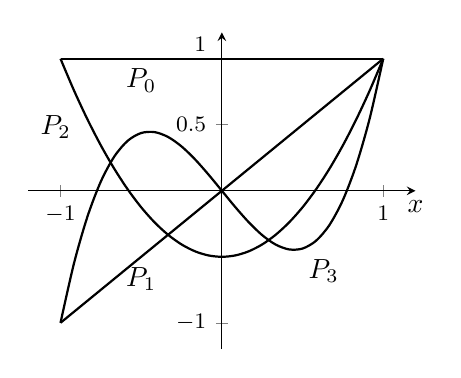
\begin{tikzpicture}[declare function={p0(\x)=1;p1(\x)=\x;p2(\x)=1/2*(3*\x^2-1);p3(\x)=1/2*(5*\x^3-3*\x);}]
\begin{axis}[small,axis lines=middle,xlabel={$x$},ylabel={}, xtick={-1,1},
 xticklabels={$-1$,$1$}, ytick={-1,0.5,1},yticklabels={$-1$,$0.5$,\raisebox{1.25em}{$1$}}, ylabel style={at={(current axis.above origin)},anchor=east},xlabel style={at={(current axis.right of origin)},anchor=north},enlargelimits]
 \addplot[thick,domain=-1:1]{p0(x)}node[pos=0.25,below]{$P_0$};
  \addplot[thick,domain=-1:1]{p1(x)}node[pos=0.25,below]{$P_1$};
   \addplot[thick,domain=-1:1,smooth]{p2(x)}node[pos=0.1,below left]{$P_2$};
    \addplot[thick,domain=-1:1,smooth]{p3(x)}node[pos=0.65,below right]{$P_3$};
 \end{axis}
\end{tikzpicture}
\caption{}
\end{subtable}
\end{table}
جدول \حوالہ{جدول_ابعاد_لیژانڈر_چند_ابتدائی} میں ابتدائی چند لیژانڈر کثیر رکنیاں پیش کی گئی ہیں۔ جیسا کہ نام سی ظاہر ہے، \عددی{P_{l}(x)} متغیر \عددی{x} کی درجہ \عددی{l} کثیر رکنی ہے، اور \عددی{l} کی قیمت طے  کرتی ہے کہ آیا یہ جفت کا طاق ہو گی۔ تاہم  \عددی{P_{l}^{m}(x)}  عموماً کثیر رکنی نہیں ہو گا؛ اور طاق \عددی{m} کی صورت میں اس میں \عددی{\sqrt{1-x^2}} کا جزو ضربی پایا جائے گا:
\begin{align*}
P_{2}^{0}(x)&=\frac{1}{2}(3x^{2}-1), \quad P_{2}^{1}(x)=(1-x^{2})^{1/2}\frac{\dif}{\dif{x}}\big[\frac{1}{2}(3x^{2}-1)\big]=3x\sqrt{1-x^{2}}, \\
P_{2}^{2}(x)&=(1-x^{2})\big(\frac{\dif}{\dif{x}}\big)^{2}\big[\frac{1}{2}(3x^{2}-1)\big]=3(1-x^{2}),
\end{align*}
وغیرہ وغیرہ۔  (اب ہمیں \عددی{P_{l}^{m}(\cos\theta)} چاہیے اور چونکہ \عددی{\sqrt{1-\cos^{2}\theta}=\sin\theta} ہوتا ہے لہٰذا \عددی{P_{l}^{m}(\cos\theta)} ہر صورت \عددی{\cos\theta} کا کثیر رکنی ہو گا جسے طاق \عددی{m} کی صورت میں
 \عددی{\sin\theta} ضرب کرے گا۔ جدول \حوالہ{جدول_ابعادی_شریک_لیژانڈر_تفاعلات} میں \عددی{\cos\theta} کے چند شریک لیژانڈر تفاعلات پیش کیے گئے ہیں۔)
\begin{table}
\caption{
چند شریک لیژانڈر تفاعلات \عددی{P_l^m(\cos\theta)}: (ا) تفاعلی روپ، (ب) ترسیمات برائے \عددی{r=P_l^m(\cos\theta)} (ان ترسیمات میں \عددی{r} آپ کو \عددی{\theta} رخ تفاعل کی  کل مقدار دیتا ہے؛  ان اشکال کو \عددی{z} محور کے گرد گھمائیں۔)
}
\label{جدول_ابعادی_شریک_لیژانڈر_تفاعلات}
\begin{subtable}{0.60\textwidth}
\centering
\begin{tabular}{ll}
$P_0^0=1$ & $P_2^0=\frac{1}{2}(3\cos^2\theta-1)$\\[0.25em]
$P_1^1=\sin\theta$ & $P_3^3=15\sin\theta(1-\cos^2\theta)$\\[0.25em]
$P_1^0=\cos\theta$ & $P_3^2=15\sin^2\theta\cos\theta$\\[0.25em]
$P_2^2=3\sin^2\theta$ & $P_3^1=\frac{3}{2}\sin\theta(5\cos^2\theta-1)$\\[0.25em]
$P_2^1=3\sin\theta\cos\theta$ & $P_3^0=\frac{1}{2}(5\cos^3\theta-3\cos\theta)$
\end{tabular}
\caption{}
\end{subtable}\hfill
\begin{subtable}{0.35\textwidth}
\centering
\begin{minipage}{0.45\textwidth}
\centering
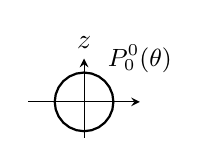
\begin{tikzpicture}[declare function={p00(\x)=1;p11(\x)=sin(90-\x); p10(\x)=cos(90-\x); p21(\x)=3*sin(90-\x)*cos(90-\x); p20(\x)=1/2*(3*cos(90-\x)^2-1); p22(\x)=3*sin(90-\x)^2;}]
\begin{axis}[clip=false,data cs=polar,axis equal,width=3cm,axis lines=middle,xlabel={},ylabel={$z$}, xtick={\empty},  xticklabels={}, ytick={\empty},yticklabels={}, ylabel style={at={(current axis.above origin)},anchor=south},xlabel style={at={(current axis.right of origin)},anchor=west},enlargelimits,ymax=1.25]
 \addplot[thick,domain=0:360]{p00(x)};
 \node[] at (rel axis cs:1,1) {\small{$P_0^0(\theta)$}};
 \end{axis}
\end{tikzpicture}
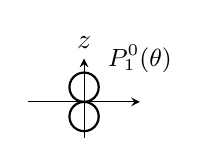
\begin{tikzpicture}[declare function={p00(\x)=1;p11(\x)=sin(90-\x); p10(\x)=cos(90-\x); p21(\x)=3*sin(90-\x)*cos(90-\x); p20(\x)=1/2*(3*cos(90-\x)^2-1); p22(\x)=3*sin(90-\x)^2;}]
\begin{axis}[clip=false,data cs=polar,axis equal,width=3cm,axis lines=middle,xlabel={},ylabel={$z$}, xtick={\empty},  xticklabels={}, ytick={\empty},yticklabels={}, ylabel style={at={(current axis.above origin)},anchor=south},xlabel style={at={(current axis.right of origin)},anchor=west},enlargelimits,ymax=1.25]
   \addplot[thick,domain=0:180,smooth]{p10(x)};
      \addplot[thick,domain=0:180,smooth]{-p10(x)};
       \node[] at (rel axis cs:1,1) {\small{$P_1^0(\theta)$}};
 \end{axis}
\end{tikzpicture}
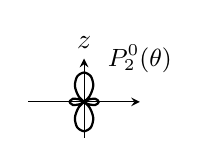
\begin{tikzpicture}[declare function={p00(\x)=1;p11(\x)=sin(90-\x); p10(\x)=cos(90-\x); p21(\x)=3*sin(90-\x)*cos(90-\x); p20(\x)=1/2*(3*cos(90-\x)^2-1); p22(\x)=3*sin(90-\x)^2;}]
\begin{axis}[clip=false,data cs=polar,axis equal,width=3cm,axis lines=middle,xlabel={},ylabel={$z$}, xtick={\empty},  xticklabels={}, ytick={\empty},yticklabels={}, ylabel style={at={(current axis.above origin)},anchor=south},xlabel style={at={(current axis.right of origin)},anchor=west},enlargelimits,ymax=1.25]
    \addplot[thick,domain=0:360,smooth]{p20(x)};
     \node[] at (rel axis cs:1,1) {\small{$P_2^0(\theta)$}};
 \end{axis}
\end{tikzpicture}
\end{minipage}\hfill
\begin{minipage}{0.45\textwidth}
\centering
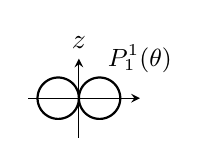
\begin{tikzpicture}[declare function={p00(\x)=1;p11(\x)=sin(90-\x); p10(\x)=cos(90-\x); p21(\x)=3*sin(90-\x)*cos(90-\x); p20(\x)=1/2*(3*cos(90-\x)^2-1); p22(\x)=3*sin(90-\x)^2;}]
\begin{axis}[clip=false,data cs=polar,axis equal,width=3cm,axis lines=middle,xlabel={},ylabel={$z$}, xtick={\empty},  xticklabels={}, ytick={\empty},yticklabels={}, ylabel style={at={(current axis.above origin)},anchor=south},xlabel style={at={(current axis.right of origin)},anchor=west},enlargelimits,xmax=1.25]
  \addplot[thick,domain=0:180,samples=100]{p11(x)};
    \addplot[thick,domain=0:180,samples=100]{-p11(x)};
     \node[] at (rel axis cs:1,1) {\small{$P_1^1(\theta)$}};
 \end{axis}
\end{tikzpicture}
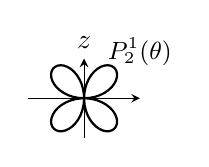
\begin{tikzpicture}[declare function={p00(\x)=1;p11(\x)=sin(90-\x); p10(\x)=cos(90-\x); p21(\x)=3*sin(90-\x)*cos(90-\x); p20(\x)=1/2*(3*cos(90-\x)^2-1); p22(\x)=3*sin(90-\x)^2;}]
\begin{axis}[clip=false,data cs=polar,axis equal,width=3cm,axis lines=middle,xlabel={},ylabel={$z$}, xtick={\empty},  xticklabels={}, ytick={\empty},yticklabels={}, ylabel style={at={(current axis.above origin)},anchor=south},xlabel style={at={(current axis.right of origin)},anchor=west},enlargelimits]
  \addplot[thick,domain=0:360,samples=100]{p21(x)};
   \node[yshift=0.25em] at (rel axis cs:1,1) {\small{$P_2^1(\theta)$}};
 \end{axis}
\end{tikzpicture}
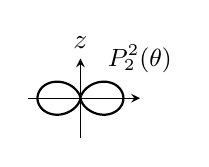
\begin{tikzpicture}[declare function={p00(\x)=1;p11(\x)=sin(90-\x); p10(\x)=cos(90-\x); p21(\x)=3*sin(90-\x)*cos(90-\x); p20(\x)=1/2*(3*cos(90-\x)^2-1); p22(\x)=3*sin(90-\x)^2;}]
\begin{axis}[clip=false,data cs=polar,axis equal,width=3cm,axis lines=middle,xlabel={},ylabel={$z$}, xtick={\empty},  xticklabels={}, ytick={\empty},yticklabels={}, ylabel style={at={(current axis.above origin)},anchor=south},xlabel style={at={(current axis.right of origin)},anchor=west},enlargelimits,xmax=3.5]
  \addplot[thick,domain=0:360,samples=100]{p22(x)};
   \node[] at (rel axis cs:1,1) {\small{$P_2^2(\theta)$}};
 \end{axis}
\end{tikzpicture}
\end{minipage}
\caption{}
\end{subtable}
\end{table}

دھیان رہے کہ صرف غیر منفی عدد صحیح \عددی{l} کی صورت میں کلیہ روڈریگیس معنی خیز ہو گا؛ مزید \عددی{|m|\textgreater{l}} کی صورت میں مساوات \حوالہ{مساوات_ابعادی_شریک_لیژانڈر_تفاعلات_تعریف} کے تحت \عددی{P_{l}^{m}=0} ہو گا۔ یوں \عددی{l} کی کسی بھی مخصوص قیمت کے لئے \عددی{m} کی \عددی{(2l+1)} ممکنہ قیمتیں ہوں گی:
\begin{align}\label{مساوات_ابعادی_انحطاطی_قیمتیں}
l=0,1,2,\dotsc;\quad m=-l,-l+1,\dotsc-1,0,1,\dotsc l-1,l
\end{align}
ذرا رکیے! مساوات  \حوالہ{مساوات_ابعادی_تھیٹا_مساوات} دو رتبی تفرقی مساوات ہے:  \عددی{l} اور \عددی{m} کی کسی بھی قیمتوں کے لئے اس کے  دو خطی غیر تابع حل ہونگے۔ باقی حل کہاں ہیں؟ \ترچھا{جواب:} یقیناً  تفرقی مساوات کے ریاضی حلوں کی  صورت میں باقی حل ضرور موجود ہوں گے تاہم  \عددی{\theta=0} اور (یا) \عددی{\theta=\pi} پر ایسے حل بے قابو بڑھتے ہیں (سوال \حوالہ{سوال_ابعادی_طبعی_نا_قابل_قبول} دیکھیں ) جس کی بنا   یہ طبعی طور  پر ناقابل قبول ہوں گے۔ 

کروی محدد میں حجمی رکن درج ذیل ہو گا
\begin{align}
\dif^{\,3}\kvec{r}=r^{2}\sin\theta\dif r\dif \theta\dif \phi
\end{align}
لہٰذا معمول زنی شرط (مساوات \حوالہ{مساوات_ابعادی_معمول_زنی_شرط}) درج ذیل روپ اختیار کرتی ہے۔
\begin{align*}
\int\abs{\psi}^{2}r^{2}\sin\theta\dif r \dif\theta\dif\phi=\int\abs{R}^{2}r^{2}\dif r\int\abs{Y}^{2}\sin\theta\dif\theta\dif\phi=1 
\end{align*}
یہاں \عددی{R} اور \عددی{Y} کو علیحدہ علیحدہ  معمول پر لانا زیادہ آسان ثابت ہوتا ہے۔
\begin{align}\label{مساوات_ابعاد_علیحدہ_معمول_زنی_شرائط}
\int_{0}^{\infty}\abs{R}^{2}r^{2}\dif r=1\quad{\text{اور}}\quad \int_{0}^{2\pi}\int_{0}^{\pi}\abs{Y}^{2}\sin\theta\dif \theta\dif \phi=1 
\end{align}
معمول شدہ  زاویائی موجی تفاعلات\حاشیہد{معمول زنی مستقل کو سوال \حوالہء{4.54} میں حاصل کیا گیا ہے؛  نظریہ زاویائی معیار حرکت میں مستعمل علامتیت کے ساتھ  ہم آہنگی کی خاطر \عددی{\epsilon} (جس کی قیمت \عددی{1} یا \عددی{-1} ہو گی) کی علامت کا انتخاب کیا گیا ہے۔ دھیان رہے کہ \عددی{Y_l^{-m}=(-1)^m(Y_l^m)^*} ہو گا۔} کو \اصطلاح{کروی ہارمونیات}\فرہنگ{کروی!ہارمونیات}\حاشیہب{spherical harmonics}\فرہنگ{spherical!harmonics} کہتے ہیں :
\begin{align}\label{مساوات_ابعادی_کروی_ہارمونیات}
Y_{l}^{m}(\theta,\phi)=\epsilon\sqrt{\frac{(2l+1)}{4\pi}\frac{(l-\abs{m})!}{(l+\abs{m})!}}e^{i{m\phi}}P_{l}^{m}(\cos\theta 
\end{align}
جہاں \عددی{m\geq0} کے لئے \عددی{\epsilon=(-1)^{m}}  اور \عددی{m\leq0}  کے لئے \عددی{\epsilon=1} ہو گا۔ جیسا کہ ہم بعد میں ثابت کریں گے، کروی ہارمونیات عمودی ہیں لہٰذا درج ذیل ہو گا۔
\begin{align}\label{مساوات_ابعادی_کروی_ہارمونی_عمودیت}
\int_{0}^{2\pi}\int_{0}^{\pi}[Y_{l}^{m}(\theta,\phi)]^*[Y_{l'}^{m'}(\theta,\phi)]\sin\theta\dif\theta\dif\phi=\delta_{ll'}\delta_{mm'} 
\end{align}
 جدول \حوالہ{جدول_ابعادی_کروی_ہارمونیات} میں چند ابتدائی  کروی ہارمونیات پیش کیے گئے ہیں۔ تاریخی وجوہات کی بنا \عددی{l} کو \اصطلاح{اسّمتی کوانٹائی عدد}\فرہنگ{کوانٹائی عدد!اسّمتی}\حاشیہب{azimuthal quantum number}\فرہنگ{quantum number!azimuthal} جب کہ \عددی{m} کو \اصطلاح{مقناطیسی کوانٹائی عدد}\فرہنگ{کوانٹائی عدد!مقناطیسی}\حاشیہب{magnetic quantum number}\فرہنگ{quantum number!magnetic} کہتے ہیں۔
\begin{table}
\caption{ابتدائی چند کروی ہارمونیات، \عددی{Y_l^m(\theta,\phi)}}
\label{جدول_ابعادی_کروی_ہارمونیات}
\renewcommand{\arraystretch}{2} 
\centering
\begin{tabular}{ll}
$Y_0^0=(\frac{1}{4\pi})^{1/2}$ & $Y_2^{\pm 2}=(\frac{15}{32\pi})^{1/2}\sin^2\theta e^{\pm 2 i \phi}$\\
$Y_1^0=(\frac{3}{4\pi})^{1/2}\cos\theta$ & $Y_3^0=(\frac{7}{16\pi})^{1/2}(5\cos^3\theta-3\cos\theta)$\\
$Y_1^{\pm 1}=\mp(\frac{3}{8\pi})^{1/2}\sin\theta e^{\pm i\phi}$ & $Y_3^{\pm 1}=\mp(\frac{21}{64\pi})^{1/2}\sin\theta(5\cos^2\theta-1)e^{\pm i\phi}$\\
$Y_2^0=(\frac{5}{16\pi})^{1/2}(3\cos^2\theta-1)$ & $Y_3^{\pm 2}=(\frac{105}{32\pi})^{1/2}\sin^2\theta\cos\theta e^{\pm 2 i \phi}$\\
$Y_2^{\pm 1}=\mp(\frac{15}{8\pi})^{1/2}\sin\theta\cos\theta e^{\pm i\phi}$ & $Y_3^{\pm3}=\mp(\frac{35}{64\pi})^{1/2}\sin^3\theta e^{\pm 3 i \phi}$
\end{tabular}
\end{table}
\ابتدا{سوال}
مساوات \حوالہ{مساوات_ابعادی_شریک_لیژانڈر_تفاعلات_تعریف}، \حوالہ{مساوات_ابعادی_روڈریگیس} اور \حوالہ{مساوات_ابعادی_کروی_ہارمونیات} استعمال کر کے \عددی{Y_{0}^{0}} اور \عددی{Y_{2}^{1}} تیار کریں۔ تصدیق کریں کہ یہ معمول شدہ اور عمودی ہیں۔
\انتہا{سوال}
%
\ابتدا{سوال}\شناخت{سوال_ابعادی_طبعی_نا_قابل_قبول}
دکھائیں کہ \عددی{l=m=0} کے لئے
\begin{align*}
\Theta(\theta)=A\ln[\tan(\theta/2)] 
\end{align*}
 مساوات \عددی{\theta} (مساوات \حوالہ{مساوات_ابعادی_تھیٹا_مساوات}) کو مطمئن کرتی ہے۔یہ (وہ) ناقابل قبول دوسرا حل ہے؛ اس میں کیا خرابی ہے؟
\انتہا{سوال}
%
\ابتدا{سوال}
مساوات \حوالہ{مساوات_ابعادی_کروی_ہارمونیات} استعمال کر کے \عددی{Y_{l}^{l}(\theta,\phi)} اور 
\عددی{Y_{3}^{2}(\theta,\phi)} تشکیل دیں۔(آپ \عددی{P_{3}^{2}} کو جو جدول \حوالہ{جدول_ابعادی_شریک_لیژانڈر_تفاعلات} سے دیکھ سکتے ہیں، جبکہ \عددی{P_{l}^{l}} آپ کو مساوات \حوالہ{مساوات_ابعادی_شریک_لیژانڈر_تفاعلات_تعریف} اور \حوالہ{مساوات_ابعادی_روڈریگیس} کی مدد سے  تشکیل دینا ہو گا۔) تصدیق کیجیے کہ  \عددی{l} اور \عددی{m} کی موزوں قیمتوں کیلئے یہ زاویائی مساوات (مساوات \حوالہ{مساوات_ابعادی_زاویائی_مساوات}) کو  مطمئن کرتے ہیں۔
\انتہا{سوال}
%
\ابتدا{سوال}
کلیہ روڈریگیس سے ابتدا کر کے  لیژانڈر  کثیر رکنیوں کی معیاری عمودیت کی شرط:
\begin{align}
\int_{-1}^{1}P_{l}(x)P_{l'}(x)\dif x=\big(\frac{2}{2l+1}\big)\delta_{ll'} 
\end{align}
اخذ کریں۔ (\ترچھا{اشارہ:} تکمل بالحصص استعمال کریں۔)
\انتہا{سوال}

\جزوحصہ{رداسی مساوات}
دھیان رہے کہ تمام کروی تشاکلی  مخفیہ کے لئے تفاعل موج کا زاویائی حصہ، \عددی{Y(\theta,\phi)}،  ایک  دوسرے جیسا ہو گا؛ مخفیے 
\عددی{V(r)} کی شکل و صورت تفاعل موج کے صرف رداسی حصہ، \عددی{R(r)}، پر اثر انداز ہو گی جسے مساوات \حوالہ{مساوات_ابعاد_رداسی_الف} تعین کرتی ہے۔
\begin{align}
\frac{\dif}{\dif r}\big(r^{2}\frac{\dif R}{\dif r}\big)-\frac{2mr^{2}}{\hslash^{2}}[V(r)-E]R=l(l+1)R
\end{align}
نئے متغیرات استعمال کرتے ہوئے اس مساوات کی سادہ روپ حاصل کی جا سکتی ہے: درج ذیل لینے سے
\begin{align}\label{مساوات_ابعادی_نئے_متغیر_رداسی}
u(r)\equiv{rR(r)} 
\end{align}  
\عددی{R=u/r}، \عددی{\dif R/\dif r=[r(\dif u/\dif r)-u]/r^{2}}، \عددی{(\dif /\dif r)[r^{2}(\dif R/\dif r)]=r\dif^{\,2}u/\dif r^{2}}  لہٰذا درج ذیل ہو گا۔
\begin{align}\label{مساوات_ابعادی_رداسی}
-\frac{\hslash^{2}}{2m}\frac{\dif^{\,2}u}{\dif r^{2}}+\big[V+\frac{\hslash^{2}}{2m}\frac{l(l+1)}{r^{2}}\big]u=Eu
\end{align}
اس کو \اصطلاح{رداسی مساوات}\فرہنگ{رداسی مساوات}\حاشیہب{radial equation}\فرہنگ{radial equation} کہتے ہیں\حاشیہد{یہاں \عددی{m} کمیت کو ظاہر کرتی ہے؛ رداسی مساوات میں علیحدگی مستقل \عددی{m} نہیں پایا جاتا ہے۔} جو شکل و صورت کے لحاظ سے یک بعدی شروڈنگر مساوات (مساوات \حوالہ{مساوات_شروڈنگر_علیحدہ_دوم}) کی طرح ہے، تاہم یہاں \اصطلاح{موثر مخفیہ}\فرہنگ{مخفیہ!موثر}\حاشیہب{effective potential}\فرہنگ{potential!effective} درج ذیل ہے
\begin{align}
V_{\text{موثر}}=V+\frac{\hslash^{2}}{2m}\frac{l(l+1)}{r^{2}} 
\end{align}
 جس میں \عددی{(\hslash^{2}/2m)[l(l+1)/r^{2}]}  اضافی جزو پایا جاتا ہے جو \اصطلاح{مرکز گریز جزو}\فرہنگ{مرکز گریز جزو}\حاشیہب{centrifugal term}\فرہنگ{centrifugal term} کہلاتا ہے۔ یہ کلاسیکی میکانیات کے مرکز گریز (مجازی) قوت کی طرح، ذرہ کو (مبدا سے دور) باہر جانب دھکیلتا ہے۔ یہاں معمول زنی شرط (مساوات \حوالہ{مساوات_ابعاد_علیحدہ_معمول_زنی_شرائط}) درج ذیل روپ اختیار کرتی ہے۔ 
\begin{align}
\int_{0}^{\infty}\abs{u}^{2}\dif r=1 
\end{align}
کسی مخصوص مخفیہ \عددی{V(r)}   کے بغیر ہم آگے نہیں بڑھ سکتے ہیں۔
%==================

\ابتدا{مثال}
درج ذیل لامتناہی کروی کنواں پر غور کریں۔
\begin{align}
V(r)=\begin{cases}
0&r\le {a}\\
\infty&r>a
\end{cases} 
\end{align}
اس کے تفاعلات موج اور اجازتی توانائیاں تلاش کریں۔

\ترچھا{حل:}\quad
کنواں کے باہر تفاعل موج صفر ہے جب کے کنواں کے اندر رداسی مساوات درج ذیل ہے
\begin{align}\label{مساوات_ابعادی_مربعی_کنواں_الف}
\frac{\dif^{\,2}u}{\dif r^{2}}=\big[\frac{l(l+1)}{r^{2}}-k^{2}\big]u 
\end{align}
جہاں ہمیشہ کی طرح درج ذیل ہو گا۔
\begin{align}
k\equiv\frac{\sqrt{2mE}}{\hslash} 
\end{align}
ہم نے اس مساوات کو، سرحدی شرط \عددی{u(a)=0} مسلط کر کے، حل کرنا ہے۔ سب سے آسان صورت \عددی{l= 0} کی ہے۔
\begin{align*}
\frac{\dif^{\,2}u}{\dif r^{2}}=-k^{2}u\implies {u(r)=A\sin(kr)+B\cos(kr)} 
\end{align*}
یاد رہے،  اصل رداسی تفاعل موج \عددی{R(r)=u(r)/r} ہے اور \عددی{r\to{0}}  کی صورت میں \عددی{[\cos(kr)]/r}  بے قابو بڑھتا ہے۔یوں ہمیں \عددی{B=0} منتخب\حاشیہد{درحقیقت ہم صرف اتنا چاہتے ہیں کہ تفاعل موج معمول پر لانے کے قابل ہو؛ یہ ضروری نہیں کہ یہ متناہی ہو: مساوات \حوالہ{مساوات_ابعاد_علیحدہ_معمول_زنی_شرائط} میں \عددی{r^2} کی بنا مبدا پر \عددی{R(r)\sim 1/r} معمول پر لانے کے قابل ہے۔} کرنا ہو گا۔ اب سرحدی شرط پر پورا اترنے کے لئے ضروری ہے  کہ \عددی{\sin(ka)=0} ہو لہٰذا
 \عددی{ka=n\pi} ہو گا جہاں \عددی{n}  عدد صحیح ہے۔ ظاہر ہے کہ اجازتی توانائیاں درج ذیل ہوں گی۔ 
\begin{align}
E_{n0}&=\frac{n^{2}\pi^{2}\hslash^{2}}{2ma^{2}},&&(n=1,2,3,...). 
\end{align}
جو عین یک بعدی لامتناہی چکور کنواں کی توانائیاں ہیں (مساوات \حوالہ{مساوات_شروڈنگر_لامتناہی_چکور_کنواں_توانائیاں})۔ \عددی{u(r)}
کو معمول پر لانے سے \عددی{A=\sqrt{2/a}} حاصل ہو گا۔ زاویائی جزو (جو \عددی{Y_{0}^{0}(\theta,\phi)=1/\sqrt{4\pi}}
کی بنا غیر اہم ہے) کو ساتھ منسلک کرتے ہوئے درج ذیل حاصل ہو گا۔ 
\begin{align}
\psi_{n00}=\frac{1}{\sqrt{2\pi a}}\frac{\sin(n\pi r/a)}{r} 
\end{align}
[دھیان کیجیے کہ ساکن حالات کے نام تین \اصطلاح{کوانٹائی اعداد}\فرہنگ{کوانٹائی اعداد}\حاشیہب{quantum numbers}\فرہنگ{quantum numbers} \عددی{n}، \عددی{l} اور \عددی{m} استعمال کر کے رکھے جاتے ہیں: \عددی{\psi_{nml}(r,\theta,\phi)}؛ جبکہ توانائی، \عددی{E_{nl}}،   صرف \عددی{n} اور \عددی{l} پر منحصر ہو گی۔] 

(ایک اختیاری عدد صحیح \عددی{l} کے لئے) مساوات \حوالہ{مساوات_ابعادی_مربعی_کنواں_الف} کا عمومی حل
\begin{align}
u(r)=Arj_{l}(kr)+Brn_{l}(kr). 
\end{align}
 بہت جانا پہچانا نہیں ہے  جہاں \عددی{j_{l}(x)} رتبہ \عددی{l} کا  \اصطلاح{کروی بیسل تفاعل}\فرہنگ{بیسل!کروی تفاعل}\حاشیہب{spherical Bessel function}\فرہنگ{Bessel!spherical function} ہے اور \عددی{n_{l}(x)} رتبہ \عددی{l} کا  \اصطلاح{کروی نیومن تفاعل}\فرہنگ{نیومن!کروی تفاعل}\حاشیہب{spherical Neumann function}\فرہنگ{Neumann!spherical function}  ہے جن کی تعریفات درج ذیل ہیں۔  
\begin{align}\label{مساوات_ابعادی_تعریفات_کروی_بیسل_نیومن}
j_{l}(x)\equiv(-x)^{l}\big(\frac{1}{x}\frac{\dif}{\dif x}\big)^{l}\frac{\sin x}{x};\quad n_{l}(x)\equiv-(-x)^{l}
\big(\frac{1}{x}\frac{\dif}{\dif x}\big)^{l}\frac{\cos x}{x}
\end{align}
مثال کے طور پر درج ذیل ہوں گے، وغیرہ وغیرہ۔
\begin{align*}
j_{0}(x)&=\frac{\sin x}{x};\quad n_{0}(x)=-\frac{\cos x}{x};\\
j_1(x)&=(-x)\frac{1}{x}\frac{\dif}{\dif x}\big(\frac{\sin x}{x}\big)=\frac{\sin x}{x^{2}}-\frac{\cos x}{x};\\
j_{2}(x)&=(-x)^{2}\big(\frac{1}{x}\frac{\dif}{\dif x}\big)^{2}\frac{\sin x}{x}=x^{2}\big(\frac{1}{x}\frac{\dif}{\dif x}\big)\frac{x\cos x-\sin x}{x^{3}}\\
&=\frac{3\sin x-3x\cos x-x^2\sin x}{x^{3}}
\end{align*}
\begin{table}
\caption{
ابتدائی چند کروی بیسل اور نیومن تفاعلات، \عددی{j_n(x)} اور \عددی{n_l(x)}؛ چھوٹی \عددی{x} کے لئے متقاربی روپ۔
}
\label{جدول_ابعادی_کروی_بیسل_نیومن_تفاعلات}
\centering
\renewcommand{\arraystretch}{2} 
\begin{tabular}{ll}
\toprule
$j_0=\frac{\sin x}{x}$  &  $n_0=-\frac{\cos x}{x}$\\
$j_1=\frac{\sin x}{x^2}-\frac{\cos x}{x}$  &  $n_1=-\frac{\cos x}{x^2}-\frac{\sin x}{x}$\\
$j_2=\big(\frac{3}{x^3}-\frac{1}{x}\big)\sin x-\frac{3}{x^2}\cos x$  &  $n_2=-\big(\frac{3}{x^3}-\frac{1}{x}\big)\cos x-\frac{3}{x^2}\sin x$\\[0.5em]
\midrule
$j_l\to\frac{2^l l!}{(2l+1)!}x^l$  &  $n_l\to -\frac{(2l)!}{2^ll!}\frac{1}{x^{l+1}},\quad x\ll 1$\\
\bottomrule
\end{tabular}
\end{table}
جدول \حوالہ{جدول_ابعادی_کروی_بیسل_نیومن_تفاعلات} میں ابتدائی چند کروی بیسل اور نیومن تفاعلات پیش کیے گئے ہیں۔ متغیر \عددی{x} کی چھوٹی قیمت کے لئے جہاں
\begin{align*}
\sin x\approx x-\frac{x^{3}}{3!}+\frac{x^{5}}{5!}-\dotsb\quad \text{اور}\quad  \cos x \approx 1-\frac{x^{2}}{2!}+\frac{x^{4}}{4!}-\dotsb
\end{align*}
 ہوں گے، درج ذیل ہوں گے، وغیرہ وغیرہ۔
\begin{align*}
j_{0}(x)\approx1;\quad{n_{0}(x)\approx-\frac{1}{x}};\quad{j_{1}(x)\approx\frac{x}{3}};\quad{j_{2}(x)\approx\frac{x^{2}}{15}}; 
\end{align*}
 دھیان رہے کہ مبدا  پر بیسل تفاعلات متناہی  ہیں جبکہ مبدا پر نیومن تفاعلات بے قابو بڑھتے ہیں۔ یوں ہمیں لازماً  \عددی{B_{l}=0} منتخب کرنا ہو گا لہٰذا درج ذیل ہو گا۔
\begin{align}
R(r)=Aj_{l}(kr) 
\end{align}
اب سرحدی شرط \عددی{R(a)=0} کو مطمئن کرنا باقی ہے۔ ظاہر ہے کہ \عددی{k} کو درج ذیل کے تحت منتخب کرنا ہو گا
\begin{align}
j_{l}(ka)=0
\end{align}
یعنی \عددی{l} رتبی کروی بیسل تفاعل کا \عددی{(ka)} ایک صفر ہو گا۔ اب بیسل تفاعلات ارتعاشی ہیں (شکل \حوالہء{4.2} دیکھیں)؛ ہر ایک کے لامتناہی تعداد  صفر پائے جاتے ہیں۔ تاہم (ہماری بدقسمتی سے) یہ ایک جیسے فاصلوں پر نہیں پائے جاتے ہیں (جیسا کہ نقاط \عددی{n} یا نقاط
\عددی{n\pi}، وغیرہ پر)؛ انہیں اعدادی تراکیب سے حاصل کرنا ہو گا۔ بہرحال سرحدی شرط کے تحت درج ذیل ہو گا
\begin{align}
k=\frac{1}{a}\beta_{nl} 
\end{align}
جہاں \عددی{\beta_{nl}} رتبہ  \عددی{l}   کروی بیسل تفاعل کا \عددی{n} واں صفر   ہو گا۔ یوں اجازتی توانائیاں 
\begin{align}\label{مساوات_ابعاد_کروی_کنواں_اجازتی_توانائیاں}
E_{nl}=\frac{\hslash^{2}}{2ma^{2}}\beta_{nl}^{2}. 
\end{align}
اور تفاعلات موج درج ذیل ہوں گے 
\begin{align}
\psi_{nlm}(r,\theta,\phi)=A_{nl}j_{l}(\beta_{nl}r/a)Y_{l}^{m}(\theta,\phi). 
\end{align}
جہاں مستقل \عددی{A_{n1}} کا تعین معمول زنی سے کیا جاتا ہے۔چونکہ \عددی{l} کی ہر ایک قیمت کے لئے \عددی{m} کی \عددی{(2l+1)}
مختلف قیمتیں پائی جاتی ہیں لہٰذا توانائی کی ہر سطح \عددی{(2l+1)} گنّا انحطاطی ہو گی (مساوات \حوالہ{مساوات_ابعادی_انحطاطی_قیمتیں} دیکھیں)۔
\انتہا{مثال}
%===============
\ابتدا{سوال}
\begin{enumerate}[a.]
\item
کروی نیومن تفاعلات \عددی{n_{1}(x)} اور \عددی{n_{2}(x)} کو (مساوات \حوالہ{مساوات_ابعادی_تعریفات_کروی_بیسل_نیومن}) میں پیش کی گئی تعریفات سے تیار کریں۔
\item
سائن اور کوسائن کو پھیلا کر \عددی{x\ll1} کے لئے كارآمد  \عددی{n_{1}(x)} اور \عددی{n_{2}(x)} کے  تخمینی کلیات  اخذ کریں۔تصدیق کریں کہ یہ مبدا پر بےقابو بڑھتے ہیں۔
\end{enumerate}
\انتہا{سوال}
%
\ابتدا{سوال}
\begin{enumerate}[a.]
\item
 تصدیق کریں کہ \عددی{V(r)=0} اور \عددی{l=1} کے لئے \عددی{Arj_{l}(kr)} رداسی مساوات کو مطمئن کرتا ہے۔
\item
لامتناہی کروی کنواں کیلئے \عددی{l=1} کی صورت میں اجازتی توانائیاں ترسیم کی مدد سے تعین کریں۔ دکھائیں کہ \عددی{n} کی بڑی قیمت کے لئے 
\عددی{E_{n1}\approx(\hslash^{2}\pi^{2}/2ma^{2})(n+1/2)^{2}} ہو گا۔(\ترچھا{اشارہ:} پہلے  
\عددی{j_{1}(x)=0\implies {x}=\tan x} دکھائیں۔ اس کے بعد \عددی{x} اور \عددی{\tan x} کو ایک ساتھ ترسیم کرتے ہوئے ان کے نقاط تقاطع تلاش کریں۔)
\end{enumerate}
\انتہا{سوال}
%
\ابتدا{سوال}
 ایک ذرہ جس کی کمیت \عددی{m} ہے کو \ترچھا{متناہی} کروی کنواں:
\begin{align*}
V(r)=\begin{cases}-V_{0}&r\le a\\0&r>a\\\end{cases} 
\end{align*}
میں رکھا جاتا ہے۔ اس کا زمینی حال، \عددی{l=0}  کے لئے،  رداسی مساوات کے حل سے حاصل کریں۔ دکھائیں کے
\عددی{V_{0}a^{2}<\pi^{2}\hslash^{2}/8m} کی صورت میں کوئی مقید حال نہیں پایا جائے گا۔
\انتہا{سوال}
%======================
\حصہ{ہائیڈروجن جوہر}
ہائیڈروجن جوہر بار \عددی{e} کے  ایک بھاری پروٹان جس کے گرد بار \عددی{-e} کا ایک ہلکا الیکٹران طواف کرتا ہو پر مشتمل ہوتا ہے۔ پروٹان بنیادی طور پر ساکن رہتا ہے (جسے ہم مبدا پر تصور کر سکتے ہیں)۔  ان دونوں کے مخالف بار کے بیچ قوت کشش پائی جاتی ہے جو انہیں اکٹھے رکھتی ہے  (شکل \حوالہء{4.3} دیکھیں)۔  قانون کولمب کے تحت مخفی توانائی درج ذیل ہو گی  
 \begin{align}\label{مساوات_ابعادی_کولمب_مخفیہ}
V(r)=-\frac{e^{2}}{4\pi\epsilon_{0}}\frac{1}{r} 
\end{align}
لہٰذا رداسی مساوات \حوالہ{مساوات_ابعادی_رداسی} درج ذیل روپ اختیار کرے گی۔
\begin{align}\label{مساوات_ابعادی_رداسی_کولمب}
-\frac{\hslash^{2}}{2m}\frac{\dif^{\,2}{u}}{\dif r^{2}}+\big[-\frac{e^{2}}{4\pi\epsilon_{0}}\frac{1}{r}+\frac{\hslash^{2}}{2m}\frac{l(l+1)}{r^{2}}\big]u=Eu 
\end{align}
 ہم نے اس مساوات کو  \عددی{u(r)}   کے لئے حل کر کے اجازتی توانائیاں \عددی{E} تعین کرنی ہیں۔  ہائیڈروجن جوہر کا حل نہایت اہم ہے لہٰذا میں اس کو، ہارمونی مرتعش کے تحلیلی حل کی ترکیب سے، قدم با قدم حل کر کے پیش کرتا ہوں۔ (جس قدم پر آپ کو دشواری پیش آئے، حصہ \حوالہ{حصہ_شروڈنگر_تحلیلی_ترکیب} سے مدد لیں جہاں مکمل تفصیل پیش کی گئی ہے۔)  کولمب مخفیہ، مساوات \حوالہ{مساوات_ابعادی_کولمب_مخفیہ}،    (\عددی{E>0} کے لئے)  \ترچھا{استمراریہ} حالات، جو الیکٹران پروٹون بکھراو کو ظاہر کرتے ہیں، تسلیم کرنے کے ساتھ ساتھ غیر مسلسل \ترچھا{مقید} حالات، جو ہائیڈروجن جوہر کو ظاہر کرتے ہے، بھی تسلیم کرتا ہے۔ ہماری دلچسپی موخر الذکر میں ہے۔

\جزوحصہ{رداسی تفاعل موج}
 سب سے پہلے نئی علامتیں متعارف کرتے ہوئے مساوات کی بہتر (صاف) صورت حاصل کرتے ہیں۔ درج ذیل متعارف کر کے (جہاں مقید حالات کے لئے \عددی{e} منفی ہونے کی وجہ سے \عددی{\kappa }  حقیقی ہو گا)
 \begin{align}\label{مساوات_ابعادی_متعارف_الف}
\kappa \equiv \frac{\sqrt{-2mE}}{\hslash} 
\end{align}
 مساوات \حوالہ{مساوات_ابعادی_رداسی_کولمب} کو \عددی{E} سے تقسیم کرنے سے
\begin{align*}
\frac{1}{\kappa ^{2}}\frac{\dif^{\,2}{u}}{\dif{r^{2}}}=\big[1-\frac{me^{2}}{2\pi\epsilon_{0}\hslash^{2}\kappa }\frac{1}{(\kappa r)}+\frac{l(l+1)}{(\kappa r)^{2}}\big]u 
\end{align*}
حاصل ہو گا جس کو دیکھ کر ہمیں خیال آتا ہے کہ ہم درج ذیل علامتیں متعارف کریں 
\begin{align}\label{مساوات_ابعادی_متعارف_ب}
\rho\equiv \kappa r, \quad \rho_{0}\equiv\frac{me^{2}}{2\pi\epsilon_{0}\hslash^{2}\kappa } 
\end{align}
لہٰذا درج ذیل لکھا جائے گا۔
\begin{align}\label{مساوات_ابعادی_رداسی_کولمب_نئے_متغیرات}
\frac{\dif^{\,2}{u}}{\dif{\rho^{2}}}=\big[1-\frac{\rho_{0}}{\rho}+\frac{l(l+1)}{\rho^{2}}\big]u 
\end{align}

اس کے بعد ہم حالات کی متقاربی روپ پر غور کرتے ہیں۔ اب \عددی{\rho\to\infty} کرنے سے قوسین کے اندر مستقل جزو غالب ہو گا لہٰذا (تخمیناً) درج ذیل لکھا جا سکتا ہے۔
\begin{align*}
\frac{\dif^{\,2}{u}}{\dif{\rho^{2}}}=u 
\end{align*}
اس کا عمومی حال درج ذیل ہے
\begin{align}\label{مساوات_ابعاد_عمومی_حل_بے_قابو}
u(\rho)=Ae^{-\rho}+Be^{\rho} 
\end{align}
تا ہم  (\عددی{\rho\to\infty} کی صورت میں) \عددی{e^{\rho}} بے قابو بڑھتا ہے لہٰذا ہمیں \عددی{B=0} لینا ہو گا۔ یوں \عددی{\rho}
کی بڑی قیمتوں کے لیے درج  ذیل ہو گا۔
\begin{align}
u(\rho)\sim Ae^{-\rho} 
\end{align}
اس کے برعکس \عددی{\rho\to 0} کی صورت میں مرکز گریز جزو غالب ہو گا؛\حاشیہد{یہ دلیل \عددی{l=0} کی صورت میں کارآمد نہیں ہو گی (اگرچہ مساوات \حوالہ{مساوات_ابعادی_ہائیڈروجن_مبدا_قریب} میں پیش نتیجہ اس صورت کے لئے بھی درست ہے)۔ بہرحال، میرا مقصد نئی علامتیت (مساوات \حوالہ{مساوات_ابعادی_نئی_علامتیت}) کے استعمال کے لئے راستہ ہموار کرنا ہے۔} لہٰذا تخمیناً  درج ذیل لکھا جا سکتا ہے۔ 
\begin{align*}
\frac{\dif^{\,2}{u}}{\dif{\rho^{2}}}=\frac{l(l+1)}{\rho^{2}}u 
\end{align*}
 جس کا عمومی حل (تصدیق کیجیے) درج ذیل ہو گا
 \begin{align*}
u(\rho)=C\rho^{l+1}+D\rho^{-l} 
\end{align*}
 تاہم  (\عددی{\rho\to0}  کی صورت میں)  \عددی{\rho^{-l}}  بے قابو بڑھتا ہے لہٰذا \عددی{D=0}  ہو گا۔ یوں  \عددی{\rho}  کی چھوٹی قیمتوں کے لیے درج ذیل ہو گا۔
 \begin{align}\label{مساوات_ابعادی_ہائیڈروجن_مبدا_قریب}
u(\rho)\sim C\rho^{l+1} 
\end{align}

  اگلے قدم پر متقاربی رویہ  کو چھیلنے کی خاطر  نیا تفاعل \عددی{v(\rho)}:
  \begin{align}\label{مساوات_ابعادی_نئی_علامتیت}
u(\rho)=\rho^{l+1}e^{-\rho}v(\rho) 
\end{align}
  اس امید سے متعارف کرتے ہے کہ    \عددی{u(\rho)}     سے  \عددی{v(\rho)} زیادہ سادہ ہو گا۔ ابتدائی نتائج 
\begin{align*}
\frac{\dif u}{\dif \rho}=\rho^l e^{-\rho} \big[(l+1-\rho)v+\rho\frac{\dif v}{\dif \rho}\big]
\end{align*}
اور
\begin{align*}
\frac{\dif^{\,2}u}{\dif \rho^2}=\rho^le^{-\rho}\big\{\big[-2l-2+\rho+\frac{l(l+1)}{\rho}\big]v+2(l+1-\rho)\frac{\dif v}{\dif \rho}+\rho\frac{\dif^{\,2}v}{\dif \rho^2}\big\}
\end{align*}
خوش آئین نظر نہیں آتے ہیں۔   اس طرح \عددی{v(\rho)} کی صورت میں رداسی مساوات (مساوات \حوالہ{مساوات_ابعادی_رداسی_کولمب_نئے_متغیرات})   درج ذیل روپ اختیار کرتی ہے۔
  \begin{align}\label{مساوات_ابعادی_رداسی_نئی_روپ}
\rho\frac{\dif^{\,2}{v}}{\dif{\rho^{2}}}+2(l+1-\rho)\frac{\dif{v}}{\dif{\rho}}+[\rho_{0}-2(l+1)]v=0 
\end{align}

  آخر میں ہم فرض کرتے ہیں کہ حل،   \عددی{v(\rho)}،  کو \عددی{\rho} کا طاقتی تسلسل لکھا جا سکتا ہے۔
  \begin{align}
v(\rho)=\sum_{j=0}^{\infty}c_{j}\rho^{j} 
\end{align}
ہمیں عددی سر (\عددی{c_0}، \عددی{c_1}، \عددی{c_2}، وغیرہ) تلاش کرنے ہوں گے۔  جزو در جزو تفرق لیتے ہیں۔
\begin{align*}
\frac{\dif{v}}{\dif{\rho}}=\sum_{j=0}^{\infty}jc_{j}\rho^{j-1}=\sum_{j=0}^{\infty}(j+1)c_{j+1}\rho^{j} 
\end{align*}
[میں نے دوسرے مجموعہ میں "فرضی اشاریہ" \عددی{j} کو \عددی{j+1} کہا ہے۔ اگر آپکو یقین نہ  ہو تو اولین چند اجزاء صریحاً لکھ کر تصدیق کر لیں۔ آپ سوال اٹھا سکتے ہیں کے نیا مجموعہ \عددی{j=-1}  سے کیوں  شروع نہیں کیا گیا؛ تاہم جزو ضربی \عددی{(j+1)}  اس جزو کو ختم کرتا ہے لہٰذا ہم صفر سے بھی شروع کر سکتے ہیں۔] دوبارہ تفرق لیتے ہیں۔
\begin{align*}
\frac{\dif^{\,2}{v}}{\dif{\rho^{2}}}=\sum_{j=0}^{\infty}j(j+1)c_{j+1}\rho^{j-1} 
\end{align*}
انہیں مساوات \حوالہ{مساوات_ابعادی_رداسی_نئی_روپ} میں پر کرتے ہیں۔
\begin{multline*}
\sum_{j=0}^{\infty}j(j+1)c_{j+1}\rho^{j}+2(l+1)+\sum_{j=0}^{\infty}(j+1)c_{j+1}\rho^{j} \\
-2\sum_{j=0}^{\infty}jc_{j}\rho^{j}+[\rho_{0}-2(l+1)]\sum_{j=0}^{\infty}c_{j}\rho^{j}=0 
\end{multline*}
ایک جیسی طاقتوں کے عددی سروں کو مساوی رکھتے ہوئے
\begin{align*}
j(j+1)c_{j+1}+2(l+1)(j+1)c_{j+1}-2jc_{j}+[\rho_{0}-2(l+1)]c_{j}=0 
\end{align*}
یا
\begin{align}\label{مساوات_ابعادی_کولمب_کلیہ_توالی}
c_{j+1}=\left\{\frac{2(j+l+1)-\rho_{0}}{(j+1)(j+2l+2)}\right\}c_{j} 
\end{align}
ہو گا۔ یہ کلیہ توالی عددی سر تعین کرتے ہوئے تفاعل \عددی{v(\rho)} تعین کرتا ہے۔ ہم \عددی{c_{0}} سے شروع کر کے (جو مجموعی مستقل کا روپ اختیار کرتا ہے جسے آخر میں معمول زنی سے حاصل کیا جائے گا)، مساوات \حوالہ{مساوات_ابعادی_کولمب_کلیہ_توالی}  سے \عددی{c_{1}} تعین کرتے ہے؛ جس کو واپس اسی مساوات میں پر کر کے \عددی{c_{2}} تعین ہو گا، وغیرہ، وغیرہ۔\حاشیہد{آپ پوچھ سکتے ہیں: طاقتی تسلسل کی ترکیب \عددی{u(\rho)} پر ہی کیوں لاگو نہیں کی گئی؛ اس ترکیب کے اطلاق سے قبل متقاربی رویہ کو کیوں (جزو ضربی کی صورت میں) باہر نکالا گیا؟ درحقیقت اس کی وجہ نتائج کی خوبصورتی ہے۔جزو ضربی \عددی{\rho^{l+1}} باہر نہ نکالنے سے تسلسل کے  ابتدائی اجزاء صفر ہوں گے (پہلا غیر صفر عددی سر \عددی{c_{l+1}} ہو گا)؛ \عددی{\rho^{l+1}}  باہر نکالنے سے تسلسل کا پہلا جزو \عددی{\rho^0} حاصل ہو گا۔ اس کے برعکس جزو ضربی \عددی{e^{-\rho}}  باہر نکالنا زیادہ ضروری ہے؛ اسے باہر نہ نکالنے سے \عددی{c_{j+2}}، \عددی{c_{j+1}} اور \عددی{c_j} پر مشتمل  تین اجزائی کلیہ توالی حاصل ہوتا ہے (کر کے دیکھیں!) جس کے ساتھ کام کرنا زیادہ مشکل ثابت ہوتا ہے۔}

 آئے \عددی{j} کی بڑی قیمت (جو \عددی{\rho}  کی بڑی قیمت کے مطابقتی ہوں گے جہاں بلند طاقتیں غالب ہوں گی) کے لئے عددی سروں کی صورت دیکھے ۔ یہاں  کلیہ توالی درج ذیل کہتا ہے۔\حاشیہد{آپ پوچھ سکتے ہیں: شمار کنندہ میں \عددی{2(l+1)-\rho_0} اور نسب نما میں \عددی{2l+2} رد کرنے کی طرح \عددی{j+1} میں \عددی{1} کیوں رد نہیں کیا جاتا؟ اس تخمین میں ایسا کیا جا سکتا ہے، تاہم اسے رد نہ کرنے سے دلیل زیادہ واضح ہو گا۔ آپ \عددی{1} کو رد کر کے دیکھ سکتے ہیں کہ میں کیا کہنا چاہتا ہوں۔}
\begin{align*}
c_{j+1}\cong\frac{2j}{j(j+1)}c_{j}=\frac{2}{j+1}c_{j} 
\end{align*}
ایک لمحہ کے لیے فرض کرے کہ یہ بالکل ٹھیک ٹھیک رشتہ ہے۔ تب 
\begin{align}
c_{j}=\frac{2^{j}}{j!}c_{0} 
\end{align}
لہٰذا
\begin{align*}
v(\rho)=c_{0}\sum_{j=0}^{\infty}\frac{2^{j}}{j!}\rho^{j}=c_{0}e^{2\rho} 
\end{align*}
 اور یوں  درج ذیل ہو گا
\begin{align}
u(\rho)=c_{0}\rho^{l+1}e^{\rho} 
\end{align}
 جو   \عددی{\rho}  کی بڑی قیمتوں کے لیے  بے قابو بڑھتا ہے۔ مثبت قوت نما وہی غیر پسندیدہ متقاربی رویہ دیتا ہے جو مساوات \حوالہ{مساوات_ابعاد_عمومی_حل_بے_قابو} میں پایا گیا۔ (در حقیقت  متقاربی حل بھی رداسی مساوات کے جائز حل ہیں البتہ ہم ان میں دلچسپی نہیں رکھتے ہیں کیونکہ یہ معمول پر  لانے کے قابل نہیں ہیں۔) اس المیہ سے نجات کا صرف ایک ہی راستہ ہے؛ تسلسل کو کہیں نہ کہیں اختتام پذیر ہونا ہو گا۔ لازمی طور پر ایک ایسا زیادہ سے زیادہ عدد صحیح، \عددی{j_{\text{بلندتر}}}، پایا جائے گا جس پر درج ذیل ہو۔
 \begin{align}
c_{(j_{\text{بلندتر}}+1)}=0
\end{align}
 (یوں کلیہ توالی کے تحت باقی تمام (زیادہ بلند) عددی سر صفر ہوں گے۔)  مساوات \حوالہ{مساوات_ابعادی_کولمب_کلیہ_توالی} سے ظاہر ہے کہ درج ذیل ہو گا۔
 \begin{align*}
2(j_{\text{بلندتر}}+l+1)-\rho_{0}=0 
\end{align*}
\اصطلاح{صدر کوانٹم  عدد}\فرہنگ{کوانٹم!صدر عدد}\حاشیہب{principal quantum number}\فرہنگ{quantum!principle number}
 \begin{align}\label{مساوات_ابعادی_صدر_کوانٹائی_عدد}
n\equiv j_{\text{بلندتر}}+l+1 
\end{align}
 متعارف کرتے ہوئے درج ذیل ہو گا۔
 \begin{align}\label{مساوات_ابعادی_رو_این}
\rho_{0}=2n 
\end{align}
 اب \عددی{E} کو  \عددی{\rho_{0}}  تعین کرتا ہے (مساوات \حوالہ{مساوات_ابعادی_متعارف_الف} اور \حوالہ{مساوات_ابعادی_متعارف_ب})
 \begin{align}
E=-\frac{\hslash^{2}\kappa ^{2}}{2m}=-\frac{me^{4}}{8\pi^{2}\epsilon^{2}\hslash^{2}\rho^{2}} 
\end{align}
 لہٰذا اجازتی توانائیاں درج ذیل ہوں گی۔ 
 \begin{align}\label{مساوات_ابعادی_ہائیڈروجن_اجازتی_توانائیاں}
E_{n}&=-\big[\frac{m}{2\hslash^{2}}\big(\frac{e^{2}}{4\pi\epsilon}\big)^{2}\big]\frac{1}{n^{2}}=\frac{E_{1}}{n^{2}}, && n=1,2,3,\dotsc
\end{align}
 یہ مشہور  زمانہ \اصطلاح{کلیہ بوہر}\فرہنگ{بوہر!کلیہ}\حاشیہب{Bohr formula}\فرہنگ{Bohr formula} ہے جو غالباً پورے کوانٹم میکانیات میں  اہم ترین نتیجہ ہے۔ جناب بوہر نے \سن{1913} میں،  ناقابل استعمال کلاسیکی طبیعیات اور نیم کوانٹم میکانیات کے ذریعہ  یہ کلیہ کو اخذ کیا۔ مساوات شروڈنگر \سن{1924} میں منظر عام ہوئی۔)

 مساوات  \حوالہ{مساوات_ابعادی_متعارف_ب} اور \حوالہ{مساوات_ابعادی_رو_این} کو ملا کر درج ذیل حاصل ہو گا
\begin{align}
\kappa =\big(\frac{me^{2}}{4\pi\epsilon_{0}\hslash^{2}}\big)\frac{1}{n}=\frac{1}{an} 
\end{align}
جہاں
\begin{align}
a\equiv\frac{4\pi\epsilon_{0}\hslash^{2}}{me^{2}}=\SI{0.529e-10}{\meter}
\end{align}
\اصطلاح{رداس بوہر}\فرہنگ{بوہر!رداس}\حاشیہب{Bohr radius}\فرہنگ{Bohr!radius} کہلاتا\حاشیہد{رداس بوہر کو روایتی طور پر زیر نوشت کے ساتھ لکھا جاتا ہے: \عددی{a_0}، تاہم یہ  غیر ضروری  ہے لہٰذا میں اس کو صرف \عددی{a} لکھوں گا۔} ہے۔ یوں (مساوات \حوالہ{مساوات_ابعادی_متعارف_ب} دوبارہ استعمال کرتے ہوئے) درج ذیل ہو گا۔
\begin{align}
\rho=\frac{r}{an} 
\end{align}
ہائیڈروجن جوہر کے فضائی تفاعلات  موج کے نام تین کوانٹائی اعداد (\عددی{n}، \عددی{l} اور \عددی{m}) استعمال کر کے رکھے جاتے ہیں 
 \begin{align}
\psi_{nlm}(r,\theta,\phi)=R_{nl}(r)Y_{l}^{m}(\theta,\phi) 
\end{align}
 جہاں مساوات \حوالہ{مساوات_ابعادی_نئے_متغیر_رداسی} اور \حوالہ{مساوات_ابعادی_نئی_علامتیت} کو دیکھتے ہوئے
 \begin{align}
R_{nl}(r)=\frac{1}{r}\rho^{l+1}e^{-\rho}v(\rho) 
\end{align} 
 ہو گا  جبکہ \عددی{v(\rho)} متغیر \عددی{\rho} میں درجہ \عددی{j_{\text{بلندتر}}=n-l-1}  کا کثیر رکنی ہو گا، جس کے عددی سر  درجہ ذیل کلیہ توالی دے گا (اور پورے تفاعل کو معمول پر لانا باقی ہے)۔
 \begin{align}\label{مساوات_ابعادی_کلیہ_توالی_کولمب_مخفیہ}
c_{j+1}=\frac{2(j+l+1-n)}{(j+1)(j+2l+2)}c_{j} 
\end{align}
\اصطلاح{زمینی حال}\فرہنگ{حال!زمینی}\حاشیہب{ground state}\فرہنگ{state!ground} (یعنی کم سے کم توانائی کے حال)  کے لیے 
 \عددی{n=1} ہو گا؛ طبعی مستقلات کی  قیمتیں پر کرتے ہوئے درجہ ذیل حاصل ہو گا۔
 \begin{align}
E_{1}=-\big[\frac{m}{2\hslash^{2}}\big(\frac{e^{2}}{4\pi\epsilon}\big)^{2}\big]=\SI{-13.6}{\electronvolt}
\end{align}
 ظاہر ہوا کہ  ہائیڈروجن کی \اصطلاح{بندشی توانائی}\فرہنگ{بندشی توانائی}\حاشیہب{binding energy}\فرہنگ{binding energy} (زمینی حال میں الیکٹران کو درکار  توانائی کی وہ مقدار جو جوہر کو باردارہ بنائے)  \عددی{\SI{13.6}{\electronvolt}} ہے۔ مساوات \حوالہ{مساوات_ابعادی_صدر_کوانٹائی_عدد} کے تحت \عددی{l=0}  لہٰذا \عددی{m=0}  ہو گا (مساوات \حوالہ{مساوات_ابعادی_انحطاطی_قیمتیں} دیکھیے) یوں درجہ ذیل ہو گا۔
 \begin{align}
\psi_{100}(r,\theta,\phi)=R_{10}(r)Y_{0}^{0}(\theta,\phi) 
\end{align}
 کلیہ توالی پہلے جزو پر ہی اختتام پذیر ہوتا ہے  ( مساوات \حوالہ{مساوات_ابعادی_کلیہ_توالی_کولمب_مخفیہ} سے \عددی{j=0} کے لئے  
 \عددی{c_{1}=0}  حاصل ہوتا ہے)،  لہٰذا \عددی{v(\rho)}  ایک مستقل   \عددی{(c_{0})}   ہو گا اور  یوں درجہ ذیل ہو گا۔
   \begin{align}
R_{10}(r)=\frac{c_{0}}{a}e^{-r/a} 
\end{align}
   اس کو مساوات \حوالہ{مساوات_ابعاد_علیحدہ_معمول_زنی_شرائط} کے تحت معمول پر لانے
سے
\begin{align*}
\int_{0}^{\infty}\abs{R_{10}}^{2}r^{2}\dif{r}=\frac{\abs{c_0}^{2}}{a^{2}}\int_{0}^{\infty}e^{-2r/a}r^{2}\dif{r}=\abs{c_{0}}^{2}\frac{a}{4}=1 
\end{align*}
یعنی \عددی{c_{0}=2/\sqrt{a}} حاصل ہو گا۔ مزید \عددی{Y_0^0=\tfrac{1}{\sqrt{4\pi}}} ہے لہٰذا  ہائیڈروجن کا زمینی حال درج ذیل ہو گا۔
\begin{align}
\psi_{100}(r,\theta,\phi)=\frac{1}{\sqrt{\pi a^{3}}}e^{-r/a} 
\end{align}
اسی طرح \عددی{n=2} کے لئے توانائی
\begin{align}
E_{2}=\frac{\SI{-13.6}{\electronvolt}}{4}=\SI{-3.4}{\electronvolt}
\end{align}
ہو گی جو پہلی ہیجان حال، یا حالات کی بندشی توانائی ہے کیونکہ   \عددی{l=0} ہو سکتا ہے (جس میں \عددی{m=0} ہو گا) یا \عددی{l=1} ہو سکتا ہے (جس  کے لئے یا  \عددی{m} کی قیمت \عددی{-1}، \عددی{0} یا \عددی{+1} ہو گی)؛ یوں چار مختلف حالات کی یہی توانائی ہو گی۔
 کلیہ توالی (مساوات \حوالہ{مساوات_ابعادی_کلیہ_توالی_کولمب_مخفیہ})  \عددی{l=0} کے لئے \عددی{j=0} استعمال کرتے ہوئے \عددی{c_1=-c_0} اور \عددی{j=1} استعمال کرتے ہوئے \عددی{c_2=0} دے گا لہٰذا \عددی{v(\rho)=c_{0}(1-\rho)} اور درجہ ذیل ہو گا۔
 \begin{align}\label{مساوات_تین_ابعادی_رداسی_بیس}
R_{20}(r)=\frac{c_{0}}{2a}\big(1-\frac{r}{2a}\big)e^{-r/2a} 
\end{align}
[دھیان رہے کہ مختلف کوانٹم اعداد \عددی{l} اور \عددی{n} کے لئے پھیلاو عددی سر  \عددی{\{c_j\}}  مکمل طور پر مختلف ہونگے۔] کلیہ توالی 
  \عددی{l= 1}   کی صورت میں پہلے جزو پر تسلسل کو اختتام پذیر کرتا ہے؛  \عددی{v(\rho)} ایک مستقل ہو گا  لہٰذا درجہ ذیل حاصل ہو گا۔
   \begin{align}\label{مساوات_تین_ابعادی_رداسی_اکیس}
R_{21}(r)=\frac{c_{0}}{4a^{2}}re^{-r/2a} 
\end{align}
(ہر منفرد صورت میں \عددی{c_0} معمول زنی سے تعین ہو گا سوال \حوالہء{4.11} دیکھیں)۔

 کسی بھی اختیاری  \عددی{n} کے لئے (مساوات \حوالہ{مساوات_ابعادی_صدر_کوانٹائی_عدد} سے ہم آہنگ) \عددی{l} کی ممکنہ قیمتیں درجہ ذیل ہوں گی
\begin{align}
l=0,1,2,\cdots, n-1 
\end{align}
جبکہ ہر  \عددی{l} کے لئے  \عددی{m}  کی ممکنہ قیمتوں کی تعداد  \عددی{(2l+1)}  ہو گی (مساوات \حوالہ{مساوات_ابعادی_انحطاطی_قیمتیں})،  لہٰذا   \عددی{E_{n}}   سطح توانائی کی کل انحطاطیت درج ذیل ہو گی۔
\begin{align}
d(n)=\sum_{l=0}^{n-1}(2l+1)=n^{2} 
\end{align}
کثیر رکنی \عددی{v(\rho)} (جو مساوات \حوالہ{مساوات_ابعادی_کلیہ_توالی_کولمب_مخفیہ} کے کلیہ توالی سے حاصل ہو گی) ایک ایسا تفاعل ہے جس سے عملی ریاضی دان بخوبی واقف ہیں؛  ماسوائے معمول زنی کے، اسے درج ذیل لکھا جا سکتا ہے۔
 \begin{align}\label{مساوات_تین_ابعادی_لاگیغ_الف}
v(\rho)=L_{n-l-1}^{2l+1}(2\rho) 
\end{align}
 جہاں
  \begin{align}\label{مساوات_تین_ابعادی_لاگیغ_ب}
L_{q-p}^{p}(x)\equiv(-1)^{p}\big(\frac{\dif}{\dif{x}}\big)^{p}L_{q}(x) 
\end{align} 
 ایک \اصطلاح{شریک لاگیغ  کثیر رکنی}\فرہنگ{لاگیغ!شریک کثیر رکنی}\حاشیہب{associated Laguerre polynomial}\فرہنگ{Laguerre!associated polynomial} ہے جبکہ 
\begin{align}\label{مساوات_تین_ابعادی_لاگیغ_پ}
 L_{q}(x)\equiv e^{x}\big(\frac{\dif}{\dif{x}}\big)^{q}(e^{-x}x^{q}) 
\end{align}
\begin{table}
\caption{ابتدائی چند لاگیغ کثیر رکنیاں، \عددی{L_q(x)}}
\label{جدول_ابعاد_لاگیغ_ابتدائی_چند}
\centering
\renewcommand{\arraystretch}{1.25}
\begin{tabular}{l}
\toprule
$L_0=1$\\
$L_1=-x+1$\\
$L_2=x^2-4x+2$\\
$L_3=-x^3+9x^2-18x+6$\\
$L_4=x^4-16x^3+72x^2-96x+24$\\
$L_5=-x^5+25x^4-200x^3+600x^2-600x+120$\\
$L_6=x^6-36x^5+450x^4-2400x^3+5400x^2-4320x+720$\\
\bottomrule
\end{tabular}
\end{table}
\begin{table}
\caption{ابتدائی چند شریک لاگیغ کثیر رکنیاں، \عددی{L_{q-p}^p(x)}}
\label{جدول_ابعادی_شریک_لاگیغ_کثیر_رکنیاں}
\centering
\renewcommand{\arraystretch}{1.25}
\begin{tabular}{ll}
\toprule
$L_0^0=1$  & $L_0^2=2$\\
$L_1^0=-x+1$  &  $L_1^2=-6x+18$\\
$L_2^0=x^2-4x+2$  &  $L_2^2=12x^2-96x+144$\\
$L_0^1=1$  &  $L_0^3=6$\\
$L_1^1=-2x+4$  &  $L_1^3=-24x+96$\\
$L_2^1=3x^2-18x+18$  &  $L_2^3=60x^2-600x+1200$\\
\bottomrule
\end{tabular}
\end{table}
\begin{table}
\caption{ہائیڈروجن کے ابتدائی چند رداسی تفاعلات، \عددی{R_{nl}(r)}}
\label{جدول_ابعادی_ہائیڈروجن_رداسی_تفاعل}
\centering
\renewcommand{\arraystretch}{2}
\begin{tabular}{l}
\toprule
$R_{10}=2a^{-3/2}e^{-r/a}$\\
\midrule
$R_{20}=\frac{1}{\sqrt{2}}a^{-3/2}\big(1-\frac{1}{2}\frac{r}{a}\big)e^{-r/2a}$\\
$R_{21}=\frac{1}{\sqrt{24}}a^{-3/2}\frac{r}{a}e^{-r/2a}$\\
\midrule
$R_{30}=\frac{2}{\sqrt{27}}a^{-3/2}\big(1-\frac{2}{3}\frac{r}{a}+\frac{2}{27}\big(\frac{r}{a}\big)^2\big)e^{-r/3a}$\\
$R_{31}=\frac{8}{27\sqrt{6}}a^{-3/2}\big(1-\frac{1}{6}\frac{r}{a}\big)\big(\frac{r}{a}\big)e^{-r/3a}$\\
$R_{32}=\frac{4}{81\sqrt{30}}a^{-3/2}\big(\frac{r}{a}\big)^2e^{-r/3a}$\\
\midrule
$R_{40}=\frac{1}{4}a^{-3/2}\big(1-\frac{3}{4}\frac{r}{a}+\frac{1}{8}\big(\frac{r}{a}\big)^2-\frac{1}{192}\big(\frac{r}{a}\big)^3\big)e^{-r/4a}$\\
$R_{41}=\frac{\sqrt{5}}{16\sqrt{3}}a^{-3/2}\big(1-\frac{1}{4}\frac{r}{a}+\frac{1}{80}\big(\frac{r}{a}\big)^2\big)\big(\frac{r}{a}\big)e^{-r/4a}$\\
$R_{42}=\frac{1}{64\sqrt{5}}a^{-3/2}\big(1-\frac{1}{12}\frac{r}{a}\big)\big(\frac{r}{a}\big)^2e^{-r/4a}$\\
$R_{43}=\frac{1}{768\sqrt{35}}a^{-3/2}\big(\frac{r}{a}\big)^3e^{-r/4a}$\\
\bottomrule
\end{tabular}
\end{table}
 \عددی{q} ویں \اصطلاح{لاگیغ کثیر رکنی}\فرہنگ{لاگیغ!کثیر رکنی}\حاشیہب{Laguerre polynomial}\فرہنگ{Laguerre!polynomial} ہے۔\حاشیہد{دیگر علامتوں کی طرح ان کے لئے بھی کئی علامتیں استعمال کی جاتی ہیں۔ میں نے سب سے زیادہ مقبول علامتیں استعمال کی ہیں۔} (جدول \حوالہ{جدول_ابعاد_لاگیغ_ابتدائی_چند} میں چند ابتدائی لاگیغ  کثیر رکنیاں  پیش کی گئی ہیں؛ جدول \حوالہ{جدول_ابعادی_شریک_لاگیغ_کثیر_رکنیاں} میں چند ابتدائی شریک لاگیغ  کثیر رکنیاں پیش کئے گئی ہیں؛  جدول \حوالہ{جدول_ابعادی_ہائیڈروجن_رداسی_تفاعل} میں چند ابتدائی رداسی تفاعل امواج پیش کئے گئے ہیں جنہیں شکل \حوالہء{4.4} میں ترسیم کیا گیا ہے۔) ہائیڈروجن کے معمول شدہ تفاعلات موج درجہ ذیل ہیں۔
  \begin{align}
\psi_{nlm}=\sqrt{\big(\frac{2}{na}\big)^3\frac{(n-l-1)!}{2n[(n+l)!]^{3}}}\,e^{-r/na}\big(\frac{2r}{na}\big)^{l}[L_{n-l-1}^{2l+1}(2r/na)]Y_{l}^{m}(\theta,\phi)
\end{align}
یہ تفاعلات خوفناک نظر آتے ہیں لیکن شکوہ  نہ کیجیے گا؛ یہ اُن چند حقیقی نظاموں میں سے ایک ہے جن کا  بند روپ میں ٹھیک ٹھیک حل حاصل کرنا ممکن ہے۔  دھیان رہے، اگرچہ تفاعلات موج تینوں کوانٹائی اعداد کے تابع ہیں، توانائیوں (مساوات \حوالہ{مساوات_ابعادی_ہائیڈروجن_اجازتی_توانائیاں}) کو صرف \عددی{n} تعین کرتا ہے۔ یہ کولمب توانائی کی ایک مخصوص خاصیت ہے؛ آپ کو یاد ہو گا کہ کروی کنواں میں توانائیاں \عددی{l} پر منحصر تھیں (مساوات \حوالہ{مساوات_ابعاد_کروی_کنواں_اجازتی_توانائیاں})۔ تفاعلات موج باہمی عمودی 
\begin{align}
\int\psi_{nlm}^{*}\psi_{n'l'm'}r^{2}\sin\theta\dif r\dif\theta\dif\phi=\delta_{nn'}\delta_{ll'}\delta_{mm'} 
\end{align}
ہیں۔ یہ کروی ہارمونیات کی عمودیت (مساوات \حوالہ{مساوات_ابعادی_کروی_ہارمونی_عمودیت})  اور \عددی{(n\neq n')} کی صورت میں  \عددی{H} کی منفرد امتیازی  اقدار کے امتیازی تفاعل ہونے کی بنا ہے۔

ہائیڈروجن تفاعلات موج کی تصویر کشی آسان کام نہیں ہے۔  ماہر کیمیا ان کے ایسے کثافتی اشکال بناتے ہیں جن کی چمک  \عددی{\abs{\psi}^{2}}
کا راست متناسب ہوتی ہے (شکل \حوالہء{4.5})۔ زیادہ معلومات مستقل کثافت احتمال کی سطحوں (شکل \حوالہء{4.6}) کے اشکال دیتی ہیں (جنہیں پڑھنا  نسبتاً مشکل ہو گا)۔


\ابتدا{سوال} 
کلیه توالی( مساوات \حوالہ{مساوات_ابعادی_کلیہ_توالی_کولمب_مخفیہ})  استعمال کرتے ہو ئے  تفاعل موج   \عددی{R_{30}}، \عددی{R_{31}} اور \عددی{R_{32}} حاصل کریں ۔ انہیں معمول پر لانے کی ضرورت نہیں۔ 
\انتہا{سوال}
\ابتدا{سوال}
\begin{enumerate}[a.]
\item
مساوات  \حوالہ{مساوات_تین_ابعادی_رداسی_بیس}  میں دیے گئے \عددی{R_{20}} کو معمول پر لا کر \عددی{\psi_{200}} تیار کریں ۔
\item
مساوات  \حوالہ{مساوات_تین_ابعادی_رداسی_اکیس}  میں دیے گئے  \عددی{R_{21}}  کو معمول پر لا کر  \عددی{\psi_{211}}،  \عددی{\psi_{210}} اور  \عددی{\psi_{21-1}}  تیار کریں۔ 
\end{enumerate}
\انتہا{سوال}
\ابتدا{سوال} 
\begin{enumerate}[a.]
\item
مساوات  \حوالہ{مساوات_تین_ابعادی_لاگیغ_پ} استعمال کرتے ہوئے ابتدائی چار لاگیغ کثیر رکنیاں حاصل کریں ۔
\item
مساوات  \حوالہ{مساوات_تین_ابعادی_لاگیغ_الف}،  \حوالہ{مساوات_تین_ابعادی_لاگیغ_ب} اور \حوالہ{مساوات_تین_ابعادی_لاگیغ_پ} استعمال کرتے ہوئے  \عددی{n=5} ،    \عددی{l=2} کی صورت میں  \عددی{v(\rho)} تلاش کریں ۔
\item
کلیہ توالی( مساوات \حوالہ{مساوات_ابعادی_کلیہ_توالی_کولمب_مخفیہ})  استعمال کرتے ہوئے \عددی{n=5} ،   \عددی{l=2}  کی صورت میں  \عددی{v(\rho)} تلاش کریں۔ 
\end{enumerate}
\انتہا{سوال}
\ابتدا{سوال} 
\begin{enumerate}[a.]
\item
ہائیڈروجن جو ہر کے زمینی حال میں الیکٹران   کے لیے  \عددی{\langle r \rangle} اور \عددی{\langle r^{2} \rangle} تلاش کریں ۔  اپنے جواب کو رداس بوہر کی صورت میں لکھیں۔ 
\item
ہائیڈروجن جوہر کے زمینی حال میں الیکٹران  کے لیے  \عددی{\langle x \rangle}  اور \عددی{\langle x^{2} \rangle}  تلاش کریں۔  \ترچھا{اشاره :}  آپکو کوئی نیا تکمل حاصل کرنے کی ضرورت نہیں ۔ دھیان  رہے کہ 
  \عددی{r^{2}=x^{2}+y^{2}+z^{2}} ہو گا    ، اور ا  زمینی حال میں تشاکلی کو بروئے کار لائیں۔ 
\item
حال \عددی{n=2} ، \عددی{l=1}، \عددی{m=1} کے لیے \عددی{\langle x^{2} \rangle} تلاش کریں ۔   \ترچھا{انتباہ:}  یہ حال \عددی{x} ، \عددی{y} اور \عددی{z} کے لحاظ سے  تشاکلی نہیں ہے ۔ یہاں
\عددی{x=r\sin{\theta}\cos{\phi}}  استعمال کرنا  ہو گا۔ 
\end{enumerate}
\انتہا{سوال}
\ابتدا{سوال} 
ہائیڈروجن کے زمینی حال میں  \عددی{r} کی کون سی قیمت زیادہ محتمل ہو گی۔ ( اس کا جواب صفر نہیں ہے !)  \ترچھا{اشاره :}  آپکو پہلے  معلوم کرنا ہو گا کہ \عددی{r} اور \عددی{r+\dif{r}} کے بیچ  الیکٹران  پائے جانے کا احتمال کیا ہو گا۔
\انتہا{سوال}
\ابتدا{سوال} 
ہائیڈروجن  جوہر ساکن  حال \عددی{n=2}، \عددی{l=1}، \عددی{m=1}  اور  \عددی{n=2}، \عددی{l=1}، \عددی{m=-1}  کے درج ذیل خطی جوڑ سے ابتداء کرتا ہے ۔
\begin{align*}
\Psi(\kvec{r},0)=\frac{1}{\sqrt{2}}(\psi_{211}+\psi_{21-1})
\end{align*}
\begin{enumerate}[a.]
\item
حال \عددی{\Psi(\kvec{r},t)} تیار کریں ۔ اس کی سادہ ترین صورت حاصل کریں ۔
\item
مخفی توانائی  کی توقعاتی قیمت ی   \عددی{\langle V \rangle} تلاش کریں ۔ (کیا یہ  \عددی{t} کی  تابع ہو گی؟)  اصل کلیہ اور عدد دی جواب   کو الیکٹران وولٹ تو صورت میں پیش کریں ۔
\end{enumerate}
\انتہا{سوال}

\جزوحصہ{ہائیڈروجن  کا   طیف}
اصولی طور پر ایک ہائیڈروجن جوہر جو ساکن حال \عددی{\psi_{nlm}} میں پایا جاتا ہو  ہمیشہ کے لیے اسی حال میں رہے گا۔ تاہم اس کو (  دوسرے جوہر کے ساتھ ٹکرا کر  یا اس پر روشنی  ڈال کر)  چھیڑنے سے الیکٹران کسی دوسرے ساکن حال میں \اصطلاح{عبور}\فرہنگ{عبور}\حاشیہب{transition}\فرہنگ{transition} کر سکتا ہے ۔ یہ توانائی جذب کر کے زیادہ توانائی  حال منتقل ہو سکتا ہے یا   (عموماً   برقناطیسی   فوٹان کے  اخراج   سے)     توانائی خارج کر  کے کم توانائی  حال  منتقل ہو سکتا ہے ۔\حاشیہد{فطراً،   اس میں تابع وقت باہم  عمل پایا جائے گا جس کی تفصیل باب \حوالہ{باب_تابع_وقت_نظریہ_اضطراب} میں پیش کی جائے گی۔یہاں اصل عمل جاننا ضروری نہیں ہے۔} عملاً  ایسی چھیڑخانیاں  ہر وقت پائی جائیں گی لہٰذا عبور (جنہیں  "کوانٹم  چھلانگ" کہتے ہیں)   مستقل طور پر ہوتے  رہیں    گے، جن  کی  بنا  ہائیڈروجن  سے ہر وقت   روشنی (فوٹان)  خارج ہو گی جس کی تونائی   ابتدائی اور اختتامی حالات کی  توانائیوں  کے فرق
\begin{align}
E_{\gamma}=E_{i}-E_{f}=\SI{-13.6}{\electronvolt}\,\big(\frac{1}{n^{2}_{i}}-\frac{1}{n^{2}_{f}}\big)
\end{align}
 کے برابر ہو گا ۔
 
اب \اصطلاح{کلیہ پلانک}\فرہنگ{پلانک!کلیہ}\حاشیہب{Planck's formula}\فرہنگ{Planck's!formula}\حاشیہد{فوٹان درحقیقت برقناطیسی اخراج  کا ایک کوانٹم ہے۔یہ ایک اضافیتی  چیز ہے جس پر غیر اضافی کوانٹم میکانیات قابل استعمال نہیں ہے۔اگرچہ ہم چند مواقع پر فوٹان کی بات کرتے ہوئے کلیہ پلانک  سے اس کی توانائی حاصل کریں گے، یاد رہے کہ اس کا اس نظریہ سے کوئی تعلق نہیں جس پر ہم بات کر رہے ہیں۔}  کے تحت  فوٹان  کی توانائی اس کے تعدد کے راست تناسب ہو گی:
\begin{align}
E_{\gamma}=h\nu
\end{align}
جبکہ   \اصطلاح{  طول موج}\فرہنگ{طول موج}    \عددی{\lambda=c/\nu} ہے لہٰذا درج ذیل ہو گا۔
\begin{align}\label{مساوات_تین_ابعادی_رڈبرگ_کلیہ}
\frac{1}{\lambda}=R\big(\frac{1}{n^{2}_{f}}-\frac{1}{n^{2}_{i}}\big)
\end{align}
جہاں 
\begin{align}
R\equiv \frac{m}{4\pi{c}\hslash^{3}}\big(\frac{e^{2}}{4\pi\epsilon_{o}}\big)^{2}=\SI{1.097e7}{\per\meter}
\end{align}
\اصطلاح{رڈبرگ  مستقل}\فرہنگ{رڈبرگ}\حاشیہب{Rydberg constant}\فرہنگ{Rydberg!constant} کہلاتا ہے ۔ مساوات \حوالہ{مساوات_تین_ابعادی_رڈبرگ_کلیہ} ہائیڈروجن کے طیف کا  \اصطلاح{کلیہ رڈبرگ}\فرہنگ{رڈبرگ!کلیہ}\حاشیہب{Rydberg formula}\فرہنگ{Rydberg!formula}  ہے ۔ یہ کلیہ انیسویں  صدی میں تجرباتی طور پر اخذ کیا گیا ۔نظریہ بوہر  کی سب سے بڑی فتح  اس کلیے کا حصول ہے جو قدرت کے بنیادی مستقلات  کی صورت میں \عددی{R}  کی قیمت دیتا ہے۔ زمینی حال  \عددی{(n_{f}=1)}  میں عبور،   بالائے بصری خطہ میں پائے  جاتے  ہیں  جنہیں    طیف پیمائی کار  \اصطلاح{لیمان تسلسل}\فرہنگ{تسلسل!لیمان}\حاشیہب{Lyman series}\فرہنگ{series!Lyman} کہتے ہیں۔ پہلی  ہیجان  حال  \عددی{(n_{f}=2)}
میں عبور،     دکھائی دینے والے خطہ میں  روشنی پیدا  کرتے  ہیں  جسے  \اصطلاح{بالمر تسلسل}\فرہنگ{تسلسل!بالمر}\حاشیہب{Balmer series}\فرہنگ{series!Balmer} کہتے ہیں۔  اسی طرح   \عددی{n_{f}=3}
میں  عبور،  \اصطلاح{پاسشن تسلسل}\فرہنگ{تسلسل!پاسشن}\حاشیہب{Paschen series}\فرہنگ{series!Paschen} دیتے ہیں  جو  زیر  بصری شعاع ہے، وغیرہ وغیرہ  (شکل\حوالہء{ 4.7}  دیکھیں)۔  (  رہائشی حرارت پر زیادہ تر  ہائیڈروجن  جوہر زمینی حال میں ہونگے؛ اخراجی طیف حاصل کرنے کی خاطر آپکو پہلے مختلف  ہیجان  حالات میں الیکٹران  آباد کرنے ہوں گے؛  ایسا عموماً گیس میں برقی شعلہ   پیدا کر کے کیا جاتا ہے۔)
 %===========================
\ابتدا{سوال}
ہائیڈروجن جوہر \عددی{Z} پروٹان  کے مرکزہ کے گرد طواف کرتے ہوئے  ایک  الیکٹران  پر مشتمل  ہے۔(از  خود ہائیڈروجن  میں  \عددی{Z=1}    جبکہ    باردارہ\اصطلاح{  ہیلیم}\فرہنگ{ہیلیم}\حاشیہب{Helium}\فرہنگ{Helium}  میں  \عددی{Z=2} اور دہری باردارہ   \اصطلاح{لتھیم }\فرہنگ{لتھیم}\حاشیہب{Lithium}\فرہنگ{Lithium} میں  \عددی{Z=3}  ہو گا،  وغیرہ وغیرہ ۔)   ہائیڈروجن  جوہر کی بوہر  توانائیاں  \عددی{E_{n}(Z)}،  بندشی  توانائی\عددی{E_{1}(Z)}،   رداس بوہر  \عددی{a(Z)}،  اور رڈبرگ  مستقل  
\عددی{R(Z)} تعین کریں ۔ (اپنے جوابات کو  ہائیڈروجن  کی متعلقہ قیمتوں کے لحاظ سے پیش کریں۔)   برقناطیسی طیف کے کس خطہ میں  \عددی{Z=2} اور  \عددی{Z=3} کی صورت میں   لیمان   تسلسل پائے جائیں گے؟   \ترچھا{اشارہ :} کسی نیے  حساب کی ضرورت نہیں ہے؛   مخفیہ (  مساوات \حوالہ{مساوات_ابعادی_کولمب_مخفیہ})   میں  \عددی{e^2\to Ze^2}  ہو گا لہٰذا تمام  نتائج میں بھی یہی کچھ پر کرنا  ہو  گا  ۔
\انتہا{سوال}
%==============================
\ابتدا{سوال}
زمین اور سورج کو ہائیڈروجن  جوہر کا متبادل تجاذبی نظام تصور کریں۔
\begin{enumerate}[a.]
\item
 مساوات  \حوالہ{مساوات_ابعادی_کولمب_مخفیہ}  کی جگہ مخفی توانائی تفاعل کیا  ہو گا ؟  (زمین کی کمیت  \عددی{m} جبکہ سورج کی کمیت \عددی{M} لیں۔)
\item
اس نظام کا   "رداس بوہر"  \عددی{a_{g}}  کیا ہو گا؟ اس کی عددی قیمت تلاش کریں ۔
\item
تجاذبی کلیہ  بوہر  لکھ کر  رداس  \عددی{r_0} کے مدار میں سیارہ  کے کلاسیکی توانائی کو  \عددی{E_n} کے برابر رکھ کر  دکھائیں کہ \عددی{n=\sqrt{r_0/a_g}} ہو گا۔ اس سے زمین کے کوانٹائی  عدد  \عددی{n}کی اندازاً قیمت تلاش کریں ۔
\item
فرض کریں  زمین  اگلی نچلی سطح   \عددی{(n-1)} میں عبور کرتی  ہے۔  کتنی توانائی  کا اخراج ہو گا؟  جواب   جاول   میں دیں ۔خارج   فوٹان(یا   زیادہ ممکنہ طور پر \اصطلاح{گریویٹان})   کا طول موج کیا ہو گا؟ ( اپنے جواب کو نوری سالوں میں پیش کریں۔ کیا یہ حیرت انگیز  نتیجہ محض ایک اتفاق ہے ۔)
\end{enumerate}
\انتہا{سوال}

\حصہ{زاویائی معیار حرکت}
ہم دیکھ چکے ہیں کہ ہائیڈروجن جو ہر کے ساکن حالات کو تین کوانٹائی اعداد \عددی{n}،  \عددی{l} اور \عددی{m} کے لحاظ سے نام دیا جاتا ہے ۔ صدر کوانٹم عدد  \عددی{(n)} حال کی توانائی تعین کرتا ہے  (مساوات  \حوالہ{مساوات_ابعادی_ہائیڈروجن_اجازتی_توانائیاں})؛  ہم دیکھیں گے کہ \عددی{l} اور \عددی{m} مداری زاویائی معیار حرکت سے تعلق رکھتے ہیں ۔ کلاسیکی نظریہ میں وسطی قوتیں،  توانائی اور معیار حرکت بنیادی بقائی مقداریں ہیں ،  اور یہ حیرت کی  بات نہیں  کہ کوانٹم میکانیات میں  زاویائی معیار حرکت( اس سے بھی زیادہ ) اہمیت  رکھتا ہے ۔

 کلاسیکی طور پر  (مبدا کے لحاظ سے)  ایک ذرہ کی زاویائی معیار حرکت درج ذیل کلیہ دیتا ہے 
\begin{align}
\kvec{L}=\kvec{r}\times\kvec{p}
\end{align}
جس کے تحت درج ذیل ہو گا۔
\begin{align}
L_{x}=yp_{z}-zp_{y}, \quad\quad L_{y}=zp_{x}-xp_{z}, \quad \quad L_{z}=xp_{y}-yp_{x}
\end{align}
ان کے متعلقہ کوانٹم عاملین معیاری نسخہ \عددی{p_x\to-i\hslash\partial/\partial x}، \عددی{p_y\to-i\hslash\partial/\partial y}،  \عددی{p_z\to-i\hslash\partial/\partial z}  سے حاصل ہوں گے۔ باب   \حوالہ{باب_غیر_تابع_وقت_شروڈنگر_مساوات} میں ہم نے ہارمونی مرتعش کے اجازتی  توانائیوں کو خالص الجبرائی ترکیب سے حاصل کیا۔  اگلے  حصہ میں  الجبرائی ترکیب  استعمال کرتے ہوئے زاویائی معیار حرکت  عاملین کے امتیازی اقدار حاصل کیے جائیں گے۔ یہ ترکیب،  عاملین کے  مقلبیت  تعلقات پر مبنی ہے ۔ اس کے بعد ہم امتیازی تفاعلات حاصل کریں گے جو  زیادہ دشوار کام ہے۔

\جزوحصہ{امتیازی اقدار}
عاملین \عددی{L_{x}} اور \عددی{L_{y}} آپس میں غیر مقلوب  ہیں۔ درحقیقت درج ذیل ہو گا۔
\begin{gather}
\begin{aligned}
[L_{x},L_{y}]&=[yp_{z}-zp_{y},zp_{x}-xp_{z}]\\
&=[yp_{z},zp_{x}]-[yp_{z},xp_{z}]-[zp_{y},zp_{x}]+[zp_{y},xp_{z}]\\
\end{aligned}
\end{gather}

%%%%%%KKKKKK the above is eq 4.97 on p172
%===========================
باضابطہ مقلبیت رشتوں مساوات 4.10 سے ہم جانتے ہیں کہ صرف \عددی{x} اور \عددی{p_x}،  \عددی{y} اور \عددی{p_y}،  \عددی{z} اور \عددی{p_z} عاملین   غیر مقلوب ہیں یوں درمیانی دو اجزا ہدف ہوں گے لہذا درج ذیل ہوگا 
\begin{align}
[L_x, L_y] = y p_x [p_z, z] + x p_y [z, p_z] = i \hslash (x p_y - y p_x) = i \hslash L_z
\end{align}
ہم \عددی{
[L_y, L_z]
} یا \عددی{
[L_z, L_x]
} بھی تلاش کر سکتے تھے تاہم انہیں علیحدہ علیحدہ معلوم کرنے کی ضرورت نہیں ہے ہم اشاریہ کی چکری ادل بدل \عددی{
(x \to y, y \to z, z \to x)
} سے فوراً درج ذیل لکھ سکتے ہیں 
\begin{align}
[L_x, L_y] = i \hslash L_z ; \quad [L_y, L_z] = i \hslash L_x ; \quad [L_z, L_x] = i \hslash L_y
\end{align}
زاویائی معیار حرکت کی یہ بنیادی مقلبیت رشتے ہیں جن سے باقی سب کچھ اخذ ہوگا

 دھیان رہے کہ \عددی{L_x} \عددی{L_y} اور \عددی{L_z} غير ہم آہنگ قابل مشاہدہ ہیں متعمم اصول عدم یقینیت مساوات 3.62 کے تحت 
\begin{align*}
\sigma_{L_x}^2 \sigma_{L_y}^2 \ge \big ( \frac{1}{2i} \langle i \hslash L_z \rangle \big )^2 = \frac{\hslash^2}{4} \langle L_z \rangle^2
\end{align*}
یا 
\begin{align}
\sigma_{L_x} \sigma_{L_y} \ge \frac{\hslash}{2} \abs{\langle L_z \rangle}
\end{align}
ہوگا یوں ایسے حالات کی تلاش جو \عددی{L_x} اور \عددی{L_y} کے بیک وقت امتیازی تفاعلات ہوں بے مقصد ہوگا اس کے برعکس کل زاویائی معیار حرکت کا مربع 
\begin{align}
L^2 \equiv L_x^2 + L_y^2 + L_z^2
\end{align} 
\عددی{L_x} کے ساتھ مقلوب ہے 
\begin{align*}
[L^2, L_x] &= [L_x^2, L_x] + [L_y^2, L_x] + [L_z^2, L_x] \\
&= L_y [L_y, L_x] + [L_y, L_x] L_y + L_z [L_z, L_x] + [L_z, L_x] L_z \\
&= L_y (- i \hslash L_z) + (- i \hslash L_z) L_y + L_z (i \hslash L_y) + (i \hslash L_y) L_z \\
&= 0
\end{align*}
مقالب  کی سادہ روپ حاصل کرنے کے لیے میں نے مساوات 3.64 استعمال کیا یہ بھی یاد رہے کہ ہر عامل اپنے  آپ کے  ساتھ مقلوب ہوگا اس سے آپ اخذ کر سکتے ہیں کہ \عددی{L_y} اور \عددی{L_z} کے ساتھ بھی \عددی{L^2} مقلوب ہوگا 
\begin{align}
[L^2, L_x] = 0, \quad [L^2, L_y] = 0, \quad [L^2, L_z] = 0
\end{align}
یا مختصراً درج ذیل ہوگا 
\begin{align}
[L^2, \kvec{L}] = 0
\end{align} 
اس طرح \عددی{\kvec{L}} کے ہر جزو کے ساتھ \عددی{L^2} ہم آہنگ ہوگا اور ہم \عددی{L^2} کا مثلًا \عددی{L_z} کے ساتھ بیک وقت امتیازی حالات تلاش کرنے کی امید رکھ سکتےہیں
\begin{align}
L^2 f = \lambda f \quad & \text{\RL{ اور}} \quad L_z f = \mu f 
\end{align}
ہم نے حصہ 2.3.1 میں ہارمونی مرتعش پر سیڑھی عامل کی ترکیب استعمال کی یہی ترکیب یہاں پر بھی استعمال کرتے ہیں 

%%%%%%
یہاں ہم درج ذیل لیتے ہیں 
\begin{align}
L \pm \equiv L_x \pm i L_y
\end{align}
\عددی{L_z} کا مقلب درج ذیل ہوگا 
\begin{align*} 
[L_z, L_{\pm}] = [L_z, L_x] \pm i [L_z, L_y] = i \hslash L_y \pm i (- i \hslash L_x) = \pm \hslash (L_x \pm i L_y)
\end{align*}
لہذا درج ذیل ہوگا 
\begin{align}
[L_z, L_{\pm}] = \pm \hslash L_{\pm}
\end{align}
اور ظاہر ہے کہ درج ذیل ہوں گے 
\begin{align}
[L^2, L_{\pm}] = 0
\end{align}
میں دعوی کرتا ہوں کہ اگر \عددی{L^2} اور \عددی{L_z} کا امتیازی تفاعل \عددی{f} ہو تب \عددی{L_{\pm} (f)} بھی ان کا امتیازی تفاعل ہوگا مساوات 4.107 کہتی ہے کہ 
\begin{align}
L^2 (L_{\pm} f) = L_{\pm} (L^2 f) = L_{\pm} (\lambda f) = \lambda (L_{\pm} f)
\end{align}
لہذا اسی امتیازی قدر \عددی{\lambda} کے لیے \عددی{
L_{\pm} f
} بھی \عددی{L^2} کا امتیازی تفاعل ہوگا جبکہ مساوات 4.106 کہتی ہے کہ 
\begin{align}
L_z (L_{\pm f}) = (L_z L_{\pm}) - L_{\pm} L_z) f + L_{\pm} L_z f = \pm \hslash L \pm f + L_{\pm} (\mu f) = (\mu \pm \hslash ) (L_{\pm} f)
\end{align}
لہذا نئی امتیازی قدر \عددی{
\mu \pm \hslash
} کے لیے \عددی{
L_{\pm} f
} \عددی{L_z} کا امتیازی تفاعل ہوگا ہم \عددی{L_{+}} کو عامل رفعت کہتے ہیں چونکہ یہ \عددی{L_{z}} کے امتیازی قدر کو \عددی{\hslash}  بڑھاتا ہے جبکہ \عددی{L_{-}} عامل تقلیل کہلاتا ہے چونکہ یہ امتیازی قیمت کو \عددی{\hslash} کم کرتا ہے یوں ہمیں \عددی{\lambda} کی کسی ایک قیمت کے لیے حالات کی ایک سیڑھی ملتی ہے جس کا ہر پایہ قریبی پایہ سے \عددی{L_{z}} کی امتیازی قدر کے لحاظ سے \عددی{\hslash} کی ایک اکائی دور ہوگا شکل 4.8 سیڑھی چڑھنے کی خاطر ہم عامل رفت کا اطلاق کرتے ہیں جبکہ سیڑھی اترنے کی خاطر ہم عامل تقلیل لاگو کرتے ہیں تاہم یہ عمل ہمیشہ کے لئے برقرار نہیں رہ سکتا ہے ہم آخرکار  ایک ایسے حال تک پہنچیں گے جس کا \عددی{z} جزو کل سے زیادہ ہوگا جو ایک ناممکن صورت ہے سیڑھی کا  بالائی   پایہ \عددی{f_{t}}  درج ذیل کو مطمئن کرے گا
\begin{align}
L_{+} f_{t} = 0
\end{align}
فرض کریں اس بالائی پایہ پر \عددی{L_z} کی امتیازی قیمت \عددی{\hslash l} ہو حرف \عددی{L} کی مناسبت آپ پر جلد آیا ہوں گی 
\begin{align}
L_z f_t = \hslash l f_{t}; \quad L^2 f_t = \lambda f_t
\end{align}
اب درج ذیل ہوگا 
\begin{align*} 
L_{\pm} L_{\mp}&= (L_x \pm i L_y) (L_x \mp i L_y) = L_x^2 + L_y^2 \mp i (L_x L_y - L_y L_x) \\
&= L^2 - L_z^2 \mp i (i \hslash L_z)
\end{align*}
یا دوسرے الفاظ میں درج ذیل ہوگا 
\begin{align}
L^2 = L_{\pm} L_{\mp} + L_z^2 \mp \hslash L_z
\end{align}
یوں 
\begin{align*}
L^2 f_t = (L_{-} L_{+} + L_z^2 + \hslash L_z) f_t = (0 + \hslash^2 l^2 + \hslash^2 l) f_t = \hslash^2 l (l + 1) f_t
\end{align*}
لہذا درج ذیل ہوگا 
\begin{align}
\lambda = \hslash^2 l (l + 1)
\end{align}
یہ ہمیں \عددی{L_z} کی امتیازی قدر کی زیادہ سے زیادہ قیمت کی صورت میں \عددی{L^2} کی امتیازی قدر دیتی ہے ساتھ ہی اسی وجہ کی بنا سیڑھی کا سب سے نچلا پایہ \عددی{f_b} پایا جائے گا جو درج ذیل کو مطمئن کرے گا 
\begin{align}
L_{-} f_b = 0
\end{align}
فرض کریں اس نچلے پایہ پر \عددی{L_z} کا امتیازی قدر \عددی{
\hslash \bar{l}
} ہو 
\begin{align}
L_z f_b = \hslash \bar{l} f_b ; \quad L^2 f_b = \lambda f_b
\end{align}
مساوات 4.112 استعمال کرتے ہوئے درج ذیل ہوگا 
\begin{align*}
L^2 f_b = (L_{+} L_{-} + L_z^2 - \hslash L_z ) f_b = (0 + \hslash^2 l^{-2} - \hslash^2 \bar{l}) f_b = \hslash^2 \bar{l} (\bar{l} - 1) f_b
\end{align*}
لہذا درج ذیل ہوگا 
\begin{align}
\lambda = \hslash^2 \bar{l} (\bar{l} - 1)
\end{align}
مساوات 4.113 اور 4.116 کا موازنہ کرنے سے \عددی{
l (l + 1) = \bar{l} (\bar{l} - 1)
} ہوگا لہذا یا \عددی{
\bar{l} = l + 1
} ہوگا جو بے معنی ہے چونکہ نچلا پایہ سب سے اوپر  (بالائی)  پایہ سے  بلند نہیں ہوگا یا درج ذیل ہوگا 
\begin{align}
\bar{l} = - l
\end{align}
ظاہر ہے کہ \عددی{L_z} کے امتیازی اقدار \عددی{m \hslash} ہونگے جہاں \عددی{ m} جس کی مناسبت آپ پر جلد عیاں ہو گی کی قیمت \عددی{ N} قدموں میں \عددی{- l} تا \عددی{+ l} ہوگی بالخصوص آپ دیکھ سکتے ہیں کہ \عددی{
l = - l + N
} لہذا \عددی{
l = N/2
} ہوگا یوں  \عددی{l} لازماً عدد صحیح یا نصف عدد صحیح ہوگا امتیازی تفاعلات کو اعداد \عددی{l} اور \عددی{ m} بیان کرتے ہیں 
\begin{align}
L^2 f_l^m = \hslash^2 l (l + 1) f_l^m ; \quad L_z f_l^m = \hslash m f_l^m
\end{align}
جہاں درج ذیل ہونگے 
\begin{align}
l = 0, 1/2, 1, 3/2, \dotsc ; \quad m = - l, - l + 1, \dotsc , l - 1, l
\end{align}
\عددی{l} کی کسی ایک قیمت کے لیے \عددی{m} کی \عددی{2l + 1} مختلف قیمتیں ہوں گی یعنی سیڑھی کے \عددی{2l + 1} پایہ ہونگے بعض اوقات اس نتیجہ کو شکل 4.9 کی طرز پر ظاہر کیا جاتا ہے جو \عددی{l = 2} کے لیے دکھایا گیا ہے یہاں تیر کا نشان ممکنہ زاویائی  معیار حرکت کو ظاہر کرتے ہیں ان تمام کی لمبائیاں  \عددی{\hslash} کی اکائیوں میں \عددی{\sqrt{l (l+ 1)}} ہوں گی جو یہاں \عددی{
\sqrt{6} = 2.45
} ہے جبکہ \عددی{m} کے \عددی{z} اجزاء \عددی{m} کی اجازتی قیمتیں \عددی{
-2, -1, 0, 1, 2
} ہیں دھیان رہے کہ ان سمتيات کے مقادیر یعنی کرہ کا رداس \عددی{z} جزو کی زیادہ سے زیادہ قیمت سے بڑی ہے عموماً \عددی{
\sqrt{l (l + 1)} > l
} ہوگا ماسوائے \عددی{
l = 0
} کی غیر اہم صورت میں آپ دیکھ سکتے ہیں کہ آپ زاویائی معیار حرکت کو سیدھا  \عددی{z} رخ نہیں رکھ سکتے ہیں پہلی نظر میں یہ ایک نا معقول بات نظر آتی ہے کیا میں \عددی{z} محدد کو زاویائی معیارحرکت سمتیہ کے رخ منتخب نہیں کر سکتا ہوں اب ایسا کرنے کی خاطر آپ کو تینوں اجزاء بیک وقت معلوم ہونے چاہیے ہیں جبکہ اصول عدم یقینیت مساوات 4.100 کہتی ہے کہ یہ ناممکن ہوگا چلو مان لیا لیکن کیا یہ ممکن نہیں ہے کہ میں اتفاقاً  \عددی{z} محدد کو \عددی{\kvec{L}} کے رخ منتخب  کر  لوں   بالکل نہیں آپ بنیادی نکتہ نہیں سمجھ پائے ہے ایسا نہیں ہے کے آپ \عددی{\kvec{L}} کے تینوں اجزاء نہیں جانتے ہیں بلکہ ایک ذرہ  کے زاویائی معیار حرکت کی سمتیہ کے تینوں اجزاء قابل تعین نہیں ہو سکتے ہیں جیسا کہ اس کا مقام اور معیار حرکت بیک وقت قابل تعین نہیں ہونگے اگر \عددی{L_z} کی قیمت قابل تعین ہو تب \عددی{L_x} اور \عددی{L_y} کی قیمتیں قابل تعین نہیں ہونگی شکل 4.9 میں سمتیات گمراہ کن ہے بہتر ہوتا کہ خطوط عرض بلند پر  ان کی لپائی کی جاتی جو یہ ظاہر کرتی کہ \عددی{L_x} اور \عددی{L_y} ناقابل تعین ہیں

 میں امید کرتا ہوں کہ میں آپ کو متاثر کرنے میں کامیاب ہوا ہونگا زاویائی معیار حرکت کے بنیادی مقلبیت رشتوں   مساوات 4.99 سے ابتدا کرتے ہوئے ہم نے صرف الجبرائی تراکیب استعمال کرکے امتیازی تفاعلات دیکھے بغیر \عددی{L^2} اور \عددی{L_z} کی امتیازی اقدار تعین کیے آئے اب امتیازی تفاعلات تیار کریں جو آپ دیکھیں گے اتنا آسان نہیں ہوگا میں کانٹے کی بات سے شروع کرتا ہوں \عددی{
f_l^m = Y_l^m
} \عددی{L^2} اور \عددی{L_z} کی امتیازی تفاعلات وہی کروی ہارمونیات ہیں جنہیں ایک دوسری راہ پر چلتے ہوئے ہم نے حصہ 4.1.2 میں حاصل کیا یہی وجہ ہے کہ میں نے حرف \عددی{l} اور \عددی{m} استعمال کیے اب میں آپ کو بتا پاوں گا کہ کروی ہارمونیات کیوں عمودی ہیں یہ الگ تھلگ امتیازی اقدار کے ہرمشی عاملین \عددی{L^2} اور \عددی{L_z} کے امتیازی تفاعلات ہیں 

\ابتدا{سوال}
عمل رفت اور عمل تقلیل \عددی{ m} کی قیمت ایک \عددی{(1)} سے تبدیل کرتے ہیں 
\begin{align}
L_{\pm} f_l^m = (A_l^m) f_l^{m \pm 1}
\end{align}
جہاں \عددی{A_l^m} کوئی مستقل ہے امتیازی تفاعلات کو معمول پر لانے کی خاطر \عددی{A_l^m} کیا ہوگا اشارہ پہلے دکھائیں کہ \عددی{L_{\pm}} اور \عددی{L_{\mp}} ایک دوسرے کے ہرمشی جوڑی دار ہے چونکہ \عددی{L_x} اور \عددی{L_y} مشہود ہیں آپ فرض کر سکتے ہیں یہ ہرمشی ہوں گے لیکن آپ چاہیں تو اس کی تصدیق کرسکتے ہیں اس کے بعد مساوات 4.112 استعمال کریں جواب 
\begin{align}
A_l^m = \hslash \sqrt{l (l +1) - m (m \pm 1)} = \hslash \sqrt{(l \mp m)(l \pm m + 1)} 
\end{align}
دیکھیے گا کے سیڑھی کی بلند ترین اور نچلے ترین پایہ پر کیا ہوگا جب آپ \عددی{f_l^l} پر \عددی{
L_{+}
} یا \عددی{f_l^{-l}} پر \عددی{L_{-}} لاگو کرتے ہیں 
\انتہا{سوال}
\ابتدا{سوال}
\begin{enumerate}[a.]
\item
مقام اور معیار حرکت کی باضابطہ  مقلبیت رشتوں   مساوات 4.10 سے شروع کرتے ہوئے درج ذیل مقالب  حاصل کریں 
\begin{align}
[[L_z , x] = i \hslash y, \quad [L_z , y] = - i \hslash x, \quad [L_z , z] = 0, \quad [L_z , p_x] = i \hslash p_y , 
\quad [L_z , p_y] = - i \hslash p_x , \quad [L_z , p_z] = 0
\end{align}
\item
ان نتائج کو استعمال کرتے ہوئے مساوات 4.96 سے  \عددی{
[L_z , L_x] = i \hslash L_y
} حاصل کریں 
\item
مقالب  \عددی{
[L_z , r^2]
} اور \عددی{
[L_z , p^2]
} کی قیمتیں تلاش کریں جہاں \عددی{
r^2 = x^2 + y^2 + z^2
} اور \عددی{
p^2 = p_x^2 + p_y^2 + p_z^2
} ہوگا
\item
اگر \عددی{V} صرف \عددی{r} کا تابع ہو تب دکھائیں کے ہیملٹنی \عددی{
H = (p^2 /2m) + V
} \عددی{\kvec{L}} کے تمام تینوں اجزاء کے ساتھ مقلوبی  ہوگا یوں \عددی{ H} \عددی{L^2} اور \عددی{L_z} باہمی ہم آہنگ مشہود ہوں گے 
\end{enumerate}
\انتہا{سوال}
\ابتدا{سوال}
\begin{enumerate}[a.]
\item
دکھائیں ایک مخفی توانائی \عددی{
V(\kvec{r})
} میں ایک ذرے کی مداری زاویائی معیارحرکت \عددی{\kvec{L}} کی توقعاتی قیمت کی شرح  تبدیلی اس کے قوت مروڑ کی توقعاتی قیمت کے برابر ہوگی 
\begin{align*}
\frac{\dif}{\dif t} \langle \kvec{L} \rangle = \langle \kvec{N} \rangle
\end{align*}
جہاں 
\begin{align*}
\kvec{N} = \kvec{r} \times (- \nabla V)
\end{align*}
یہ مسئلہ اہرنفسٹ کا مماثل گھومتا تعلق ہے 
\item
دکھائے کے کسی بھی کروی تشاکلی مخفی توانائی کے لیے \عددی{
\dif \langle \kvec{L} \rangle \dif t = 0
} ہوگا یہ زاویائی معیار حرکت کی بقا کا کوانٹم میکانی روپ ہے 
\end{enumerate}
\انتہا{سوال}

%the above is prob 4.20 (p179)
%===============

\جزوحصہ{امتیازی تفاعلات}
ہمیں سب سے پہلے \عددی{L_x}،  \عددی{L_y} اور \عددی{L_z} کو کروی محدد میں لکھنا ہوگا اب  \عددی{
\kvec{L} = (\hslash/i)(\kvec{r} \times \kvec{\nabla})
} ہے جبکہ کروی محدد میں ڈھلوان درج ذیل ہوگا 
\begin{align}
\kvec{\nabla} = \ar \frac{\partial}{\partial r} + \atheta \frac{1}{r} \frac{\partial}{\partial \theta} + \aphi \frac{1}{r \sin {\theta}} \frac{\partial}{\partial \phi}
\end{align}
جہاں \عددی{
\kvec{r} = r \ar
} ہوگا یوں درج ذیل لکھا جا سکتا ہے 
\begin{align*}
\kvec{L} = \frac{\hslash}{i} \big [ r (\ar \times \ar) \frac{\partial}{\partial r} + (\ar \times \atheta) \frac{\partial}{\partial \theta} + (\ar \times \aphi) \frac{1}{\sin \theta} \frac{\partial}{\partial \phi} \big ]
\end{align*}
اب \عددی{
(\ar \times \ar) = 0
}،  \عددی{
(\ar \times \atheta) = \aphi
} اور \عددی{
(\ar \times \aphi) = - \atheta
} ہوتے ہیں شکل 4.1 لہذا درج ذیل ہوگا 
\begin{align}
\kvec{L} = \frac{\hslash}{i} \big ( \aphi \frac{\partial}{\partial \theta} - \atheta \frac{1}{\sin \theta} \frac{\partial}{\partial \phi} \big )
\end{align}
اکائ سمتیات \عددی{\atheta} اور \عددی{\aphi} کو ان کے کارتیسی اجزاء میں لکھتے ہیں 
\begin{align}
\atheta = (\cos \theta \cos \phi) \ai + (\cos \theta \sin \phi) \aj - (\sin \theta) \ak
\end{align}
\begin{align}
\aphi = - (\sin \phi) \ai + (\cos \phi) \aj
\end{align}
یوں 
\begin{align*}
\kvec{L} = \frac{\hslash}{i} [(- \sin \phi \,\ai + \cos \phi\, \aj) \frac{\partial}{\partial \theta} - (\cos \theta \cos \phi \,\ai + \cos \theta \sin \phi \,\aj - \sin \theta \,\ak) \frac{1}{\sin \theta} \frac{\partial}{\phi}]
\end{align*}
ہوگا ظاہر ہے درج ذیل ہوں گے 
\begin{align}
L_x = \frac{\hslash}{i} \big ( - \sin \phi \frac{\partial}{\partial \theta} - \cos \phi \cot \theta \frac{\partial}{\partial \phi} \big )
\end{align}
\begin{align}
L_y = \frac{\hslash}{i} \big ( + \cos \phi \frac{\partial}{\partial \theta} - \sin \phi \cot \theta \frac{\partial}{\partial \phi} \big )
\end{align} 
\begin{align}
L_z = \frac{\hslash}{i} \frac{\partial}{\partial \phi}
\end{align} 

ہمیں آمل رفت اور امل تقلیل بھی درکار ہوں گے 
\begin{align*}
L_{\pm} = L_x \pm i L_y = \frac{\hslash}{i} \big [ (- \sin \phi \pm i \cos \phi) \frac{\partial}{\partial \theta} - (\cos \phi \pm i \sin \phi) \cot \theta \frac{\partial}{\partial \phi} \big ]
\end{align*}
چونکہ \عددی{
\cos \phi \pm i \sin \phi = e^{\pm i \phi}
} ہوتا ہے لہذا درج ذیل ہوگا 
\begin{align}
L_{\pm} = \pm \hslash e^{\pm i \phi} \big ( \frac{\partial}{\partial \theta} \pm i \cot \theta \frac{\partial}{\partial \phi} \big )
\end{align}
بالخصوص سوال 4.21(a) درج ذیل ہوگا 
\begin{align}
L_{+} L_{-} = - \hslash^2 \big ( \frac{\partial^2}{\partial \theta^2} + \cot \theta \frac{\partial}{\partial \theta} + \cot^2 \theta \frac{\partial^2}{\partial \phi^2} + i \frac{\partial}{\partial \phi} \big )
\end{align}
لہذا سوال 4.21(b) درج ذیل حاصل ہوتا ہے 
\begin{align}
L^2 = - \hslash^2 \big [ \frac{1}{\sin \theta} \frac{\partial}{\partial \theta} \big ( \sin \theta \frac{\partial}{\partial \theta} \big ) + \frac{1}{\sin^2 \theta} \frac{\partial^2}{\partial \phi^2} \big ]
\end{align}
ہم اب \عددی{
f_l^m (\theta, \phi)  
} پائين کر سکتے ہیں یہ \عددی{
L^2
} کا امتیازی تفاعل ہے جس کی امتیازی قدر \عددی{
\hslash^2 l (l + 1)
} ہے 
\begin{align*}
L^2 f_l^m = - \hslash^2 \big [ \frac{1}{\sin \theta} \frac{\partial}{\partial \theta} \big ( \sin \theta \frac{\partial}{\partial \theta} \big ) + \frac{1}{\sin^2 \theta} \frac{\partial^2}{\partial \phi^2} \big ] f_l^m = \hslash^2 l (l + 1) f_l^m
\end{align*}
یہ ٹھیک زاویائی مساوات 4.18 ہے ساتھ ہی یہ \عددی{L_z} کا امتیازی تفاعل بھی ہے جہاں اس کا امتیازی قدر \عددی{m \hslash} ہوگا 
\begin{align*}
L_z f_l^m = \frac{\hslash}{i} \frac{\partial}{\partial \phi} f_l^m = \hslash m f_l^m
\end{align*}
جوائن شمالی مساوات مساوات 4.21 کا معادل ہے ہم ان مساوات کا نظام حل کر چکے ہیں ان کا معمول شدا نتیجہ کروی ہارمونیات \عددی{
Y_l^m (\theta , \phi)
} ہے اس سے ہم یہ نتیجہ اخذ کرتے ہیں کے \عددی{L^2} اور \عددی{L_z} کے امتیازی تفاعلات کروی ہارمونیات ہونگے حصہ 4.1 میں علیحدگی متغیرات کی ترکیب سے مساوات شروڈنگر حل کرتے ہوئے ہم انجانے میں تین مقلوبی عاملین \عددی{H} \عددی{L^2} اور \عددی{L_z} کے بیک وقت امتیازی تفاعلات تیار کر رہے تھے 
\begin{align}
H \psi = E \psi , \quad L^2 \psi = \hslash^2 l (l + 1) \psi , \quad L_z \psi = \hslash m \psi
\end{align}
ہم مساوات 4.132 استعمال کرتے ہوئے مساوات شروڈنگر مساوات 4.14 کو مختصرا درج ذیل لکھ سکتے ہیں 
\begin{align*}
\frac{1}{2m r^2} \big [ - \hslash^2 \frac{\partial}{\partial r} \big ( r^2 \frac{\partial}{\partial r} \big ) + L^2 \big ]  \psi + V \psi = E \psi
\end{align*}
یہاں ایک دلچسپ صورتحال پیدا ہوتی ہے علحدگی متغیرات کی ترکیب سے امتیازی تفاعلات کی صرف عدد صحیح \عددی{l} قیمتیں مساوات 4.29 حاصل ہوئی جبکہ زاویائی معیار حرکت کی الجبرائی نظریہ \عددی{l} اور لہذا \عددی{m} بھی کی نصف عدد صحیح قیمتیں مساوات 4.119 بھی دیتی ہے آپ کا خیال ہوگا کہ نصف عدد صحیح نتائج غیر ضروری ہے لیکن جیسا آپ اگلے حصوں میں دیکھیں گے کہ یہ انتہائی زیادہ اہمیت کے حمل ہے 
\ابتدا{سوال}
\begin{enumerate}[a.]
\item
مساوات 4.130 سے مساوات 4.131 اخذ کریں اشارہ تفاعل برق استعمال کرنا نہ بھولیں 
\item
مساوات 4.129 اور 4.131 سے مساوات 4.132 اخذ کریں اشارہ مساوات 4.112 استعمال کریں 
\end{enumerate}
\انتہا{سوال} 
\ابتدا{سوال}
\begin{enumerate}[a.]
\item
حساب کیے بغیر بتائیں \عددی{
L_{+} Y_l^l
} کیا ہوگا 
\item
مساوات 4.130 کے ساتھ جزو ( الف) کا نتیجہ اور یہ جانتے ہوئے کہ \عددی{
L_z Y_l^l = \hslash l Y_l^l
} ہوگا \عددی{
Y_l^l (\theta , \phi)
} کی ایک مستقل تک معمول شدہ قیمت تلاش کریں 
\item
بلاواسطہ تکمل کے ذریعے مستقل معمول ذنی تعین کریں اپنی حتمی نتیجے کا سوال 4.5 کے نتیجے کے ساتھ موازنہ کریں 
\end{enumerate} 
\انتہا{سوال}
\ابتدا{سوال}
آپ نے سوال 4.3 میں درج ذیل دکھایا 
\begin{align*} 
Y_2^1 (\theta , \phi) = - \sqrt{15/8 \pi} \sin \theta \cos \theta e^{i \phi}
\end{align*}
عامل رفت کا \عددی{
Y_2^2 (\theta , \phi)
} پر اطلاق کریں معمول زنی کے لیے مساوات 4.121 استعمال کریں 
\انتہا{سوال}
\ابتدا{سوال}
بے کمیت کا ایک ڈنڈا جس کی لمبائی \عددی{a} ہے کے دونوں سروں پر کمیت \عددی{m}  کے ذرات بندے ہوئے ہیں يہ نظام وسط کے گرد آزادی سے تین بودی حرکت کرسکتا ہے جبکہ نظام کا وسط از  خود حرکت نہیں کرتا 
\begin{enumerate}[a.]
\item
دکھائیں کے اس نظام کی اجازتی توانائیاں درج ذیل ہو نگی 
\begin{align*}
E_n& = \frac{\hslash^2 n (n + 1)}{m a^2} ,&& n=0,1,2,\dotsc 
\end{align*}
اشارہ کلاسیکی تمنائیوں کو کل زاویائی معیار حرکت کی صورت میں لکھیں 
\item
اس نظام کی معمول شدہ امتیازی تفاعلات کیا ہوںگے اس نظام کی \عددی{n} وی توانائی سطح کی انحطاطیت کیا ہوگی 
\end{enumerate}
\انتہا{سوال}

%the above is prob 4.24 (p182)
%below is sec 4.4
\حصہ{چکر}
کلاسیکی میکانیات میں بے لچک جسم کے زاویائی معیار حرکت کے دو اقسام پائے جاتے ہیں پہلی قسم مرکز کمیت کے حرکت کے ساتھ وابستہ ہے جسے مداری \عددی{
(\kvec{L} = \kvec{r} \times \kvec{p})
} کہتے ہیں جبکہ دوسری چکر \عددی{
(\kvec{S} = I \kvec{\omega})
} جو مرکز کمیت کے گرد حرکت سے وابستہ ہے مثال کے طور پر سورج کے گرد سالانہ مدار کی بنا زمین کا مداری زاویائی معیار حرکت ہوگا جبکہ روزانہ کی بنیاد پر شمال جنوبی محور کے گرد چکر کی بنا اس کا چکری زاویائی معیار حرکت ہوگا کلاسیکی طور پر یہ فرق ہماری آسانی کے لئے ہے چونکہ حقیقتا ہر پتھر ہر پہاڑ وغیرہ جن پر زمین مشتمل ہے کا زمین کے محور کے گرد انفرادی مداری زاویائی معیارحرکت کا مجموعہ \عددی{\kvec{S}} کے برابر ہوگا کوانٹم میکانیات میں اس کا معادل پایا جاتا ہے لیکن یہاں ایک بنیادی فرق پایا جاتا ہے ہائیڈروجن کی صورت میں مرکزہ کے گرد الیکٹران کی طواف کی بنا مداری زاویائی معیار حرکت کے ساتھ ساتھ الیکٹران زاویائی معیار حرکت کی ایک دوسری روپ بھی رکھتا ہے جس کا فضا میں حرکت کے ساتھ کوئی تعلق نہیں پایا جاتا ہے لہذا اس کو مقام کے متغیرات \عددی{r} \عددی{\theta} اور \عددی{\phi} سے بیان نہیں کیا جا سکتا ہے چونکہ یہ کلاسیکی چکر کی طرح ہے لہذا اسے ہم اسی لفظ سے پکارتے ہیں یہ مماثلت یہی پر ختم ہوجاتی ہے ایک ایکٹران جہاں تک ہم جانتے ہیں کی کوئی جسامت نہیں پائی جاتی ہے اور یہ نقطی ذرا ہے لہذا اس کی چکری زاویائی معیار حرکت کو مداری زاویائی معیار حرکت پر مشتمل حصوں میں تقسیم نہیں کیا جاسکتا ہے سوال 4.25 یہاں اتنا کہنا کافی ہوگا کہ بنیادی ذرات بیرونی زاویائی معیارحرکت \عددی{\kvec{L}} کے ساتھ ساتھ اندرونی زاویائی معیار حرکت \عددی{\kvec{S}} بھی رکھتے ہیں چکر کا الجبرائی نظریہ ہو بہو مداری زاویائی معیار حرکت کی نظریہ کی طرح ہے ہم باضابطہ  مقلبیت رشتہ سے شروع کرتے ہیں 
\begin{align}
[S_x , S_y] = i \hslash S_z , \quad [S_y , S_z] = i \hslash S_x , \quad [S_z , S_x] = i \hslash S_y
\end{align}
یوں پہلے کی طرح \عددی{S^2} اور \عددی{S_z} کے امتیازی تفاعلات درج ذیل کو مطمئن کرتے ہیں 
\begin{align}
S^2 | s m \rangle = \hslash^2 s (s + 1) | s m \rangle ; \quad S_z | s m \rangle = \hslash m | s m \rangle
\end{align} 
جبکہ درج ذیل ہوگا جہاں \عددی{
S_{\pm} \equiv S_x \pm i S_y
} 
\begin{align}
S_{\pm} | s m \rangle = \hslash \sqrt{s (s + 1) - m (m \pm 1)} | s (m \pm 1) \rangle
\end{align}
تاہم یہاں امتیازی تفاعلات \عددی{\theta} اور \عددی{\phi} کے تفاعل نہیں ہیں لہذا یہ کروی ہارمونیات نہیں ہونگے اور کوئی وجہ نہیں پائی جاتی ہے کہ ہم \عددی{s} اور \عددی{m} کی نصف عدد صحیح قیمتیں قبول نہ کریں 
\begin{align} 
s = 0, 1/2, 1, 3/2, \dotsc ; \quad m = - s, - s + 1 , \dotsc , s - 1, s
\end{align}
ہم دیکھتے ہیں کہ ہر بنیادی ذرے کے \عددی{s} کی ایک مخصوص ناقابل تبدیل قیمت ہوتی ہے جسے اس مخصوص نسل کا چکر کہتے ہیں \عددی{\pi} میزون کا چکر \عددی{0} ہے الیکٹران کا چکر \عددی{1/2} پروٹان کا چکر \عددی{1} ڈیلٹا کا چکر \عددی{3/2} گریویٹون کا چکر \عددی{2} وغیرہ وغیرہ اس کے برعکس ہائیڈروجن جوہر میں ایک الیکٹرون کا مداری زاویائی معیارحرکت کوانٹم عدد \عددی{l} کوئی بھی عدد صحیح قیمت رکھ سکتا ہے جو نظام چھیڑنے سے تبدیل ہوگا تاہم کسی بھی ذرے کا \عددی{s} اٹل ہو گا جس کی بنا نظریہ چکر نسبتا سادہ ہے 
\ابتدا{سوال}
اگر الیکٹران ایک کلاسیکی ٹھوس کرہ ہوتا جس کا رداس درج ذیل ہو 
\begin{align}
r_c = \frac{e^2}{4 \pi \epsilon_0 m c ^2}
\end{align}
ہم آئنشٹائن کلیہ \عددی{
E= mc^2
} کے تحت یہ فرض کرتے ہوئے کہ الیکٹران کی کمیت اس کی برقی میدان کے توانائی کی بنا ہے الیکٹران کا کلاسیکی رداس حاصل کرتے ہیں الیکٹران کا زاویائی معیار حرکت \عددی{
(1/2) \hslash
} لیتے ہوئے خطہ استوا پر کسی نقطے کی رفتار \عددی{
\si{\meter \per \second}
} میں تلاش کریں کیا حاصل جواب معنی خیز ہے در حقیقت تجربات سے ظاہر ہے کہ الیکٹران کا رداس \عددی{
r_c
} سے بہت کم ہے کیا یہ جانتے ہوئے نتیجہ مزید غلط محسوس ہو گا 
\انتہا{سوال}


%below is sec 4.4.1 spin 1/2 (p185) till eq 4.158 (inclusive, P191)
\جزوحصہء{ \عددی{1/2} چکر}
%sec 4.4.1 spin 1/2 page 185
سادہ مادہ ( پروٹان،  نیوٹران،  الیکٹران)  کے ساتھ ساتھ \اصطلاح{کوارک}\حاشیہب{quarks}  اور تمام \اصطلاح{ لپٹان}\فرہنگ{لپٹان}\حاشیہب{leptons}\فرہنگ{leptons}  کیلۓ  \عددی{s=\tfrac{1}{2}}  ہو گا جو سب سے اہم ترین صورت ہے۔ مزید\عددی{1/2} چکر سمجھنے کے بعد زیادہ چکر کے ضوابط  دریافت کرنا نسبتاً   آسان ہے۔  صرف "دو"   عدد امتیازی تفاعلات  پائے جاتے ہیں:  پہلا \عددی{|\tfrac{1}{2}\tfrac{1}{2}\rangle}  ہے جسے  \اصطلاح{ہم میدان چکر}\فرہنگ{چکر!ہم میدان}\حاشیہب{spin up}\فرہنگ{spin up} ( یا غیر رسمی طور پر  \عددی{\uparrow}) اور دوسرا \عددی{|\tfrac{1}{2}(-\tfrac{1}{2})\rangle} ہے جس کو  \اصطلاح{مخالف میدان چکر}\فرہنگ{چکر!مخالف میدان}\حاشیہب{spin down}\فرہنگ{spin down} (\عددی{\downarrow}) کہتے ہیں۔ انہیں کو  اساس سمتیات لیتے   ہوئے   \عددی{1/2}  چکر ذرے  کے عمومی حال کو دو اجزائی قالب قطار   (یا\اصطلاح{ چکرکار}\فرہنگ{چکرکار}\حاشیہب{spinor}\فرہنگ{spinor}) سے ظاہر کر سکتے ہیں:
\begin{align}\label{مساوات_تین_بعدی_عمومی_حال_چائے}
 \chi=\begin{pmatrix} a \\ b \end{pmatrix}= a\chi_{+} + b\chi_{-} 
 \end{align}
جہاں
\begin{align} 
 \chi_{+}=\begin{pmatrix}1\\0 \end{pmatrix}
 \end{align}
ہم میدان چکر  کو ظاہر کرتا ہے اور  
\begin{align} 
 \chi_{-}=\begin{pmatrix}0 \\1 \end{pmatrix}
 \end{align}
مخالف میدان چکر کو ظاہر کرتا ہے۔

ساتھ ہی عاملین چکر   \عددی{2\times 2}  قالب ہوں گے جنہیں حاصل کرنے کی خاطر ہم ان کا  اثر  \عددی{\chi_+} اور \عددی{\chi_-} پر  دیکھتے ہیں۔  مساوات  \حوالہء{4.135}  درج ذیل کہتی ہے۔
\begin{align} \label{مساوات_تین_بعدی_ہم_میدان_خلاف_میدان}
 \bold{S}^2\chi_{+}=\frac{3}{4}\hslash^2\chi_{+}\quad \text{اور} \quad \bold{S}^2\chi_{-}= \frac{3}{4}\hslash^2 \chi_{-}
 \end{align}
ہم \عددی{ \bold{S}^2 } کو ( اب تک)  نا معلوم ارکان کا قالب 
\begin{align} 
 \bold{S}^2=\begin{pmatrix}c &d\\e & f\end{pmatrix}
 \end{align}
لکھ کر  مساوات \حوالہ{مساوات_تین_بعدی_ہم_میدان_خلاف_میدان} کی بائیں مساوات  کو درج ذیل لکھ سکتے ہیں
\begin{align*} 
   \begin{pmatrix}c\\e \end{pmatrix}= \begin{pmatrix}\tfrac{3}{4}\hslash^2 \\ 0 \end{pmatrix}\quad \text{یا}\quad \begin{pmatrix}c & d \\ e & f \end{pmatrix}
\begin{pmatrix}1\\0 \end{pmatrix}= \frac{3}{4}\hslash^2 \begin{pmatrix}\hslash \\0 \end{pmatrix}
 \end{align*}
لہٰذا \عددی{ c=\tfrac{3}{4}\hslash^2 } اور \عددی{ e=0 } ہو گا۔  مساوات \حوالہ{مساوات_تین_بعدی_ہم_میدان_خلاف_میدان} کی دائیں مساوات کے تحت
\begin{align*} 
\begin{pmatrix} d \\ f \end{pmatrix}= \begin{pmatrix}0 \\ \tfrac{3}{4}\hslash^2 \end{pmatrix} \quad \text{یا}\quad 
 \begin{pmatrix} c & d \\ e & f \end{pmatrix} \begin{pmatrix} 0 \\ 1 \end{pmatrix} = \frac{3}{4}\hslash^2
 \begin{pmatrix} 0 \\ 1 \end{pmatrix}
 \end{align*} 
 لہٰذا \عددی{ d=0 } اور \عددی{ f=\frac{3}{4}\hslash^2 } ہو گا۔  یوں درج ذیل حاصل ہوتا ہے۔
 \begin{align} 
\bold{S}^2= \frac{3}{4}\hslash^2 \begin{pmatrix} 1&0 \\ 0&1 \end{pmatrix} 
 \end{align} 
%page 174 
اسی طرح 
\begin{align} 
 \bold{S}_{z}\chi_{+}=\frac{\hslash}{2}\chi_{+}, \quad \bold{S}_{z} \chi_{-}=-\frac{\hslash}{2}\chi_{-}, 
 \end{align}
سے درج ذیل حاصل ہو گا۔
\begin{align} 
 \bold{S}_{z}= \frac{\hslash}{2}\begin{pmatrix} 1&0 \\ 0&-1 \end{pmatrix} 
 \end{align}
ساتھ ہی مساوات \حوالہء{ 4.136}  ذیل کہتی ہے۔
\begin{align*} 
 \bold{S}_{+} \chi_{-}=\hslash \chi_+, \quad \bold{S}_{-}\chi_{+}=\hslash \chi_- , \bold{S}_{+} \chi_{+}= \bold{S}_{-} \chi_{-}=0, 
 \end{align*}
لہٰذا درج ذیل ہو گا۔
\begin{align} 
 \bold{S}_{+}=\hslash\begin{pmatrix} 0&1 \\ 0&0 \end{pmatrix} , \quad \bold{S}_{-}=\hslash\begin{pmatrix}0&0 \\ 1&0 \end{pmatrix} 
 \end{align}
 اب     چونکہ \عددی{S_{\pm}=S_x{\pm}iS_y}  ہے لہٰذا    \عددی{S_x=\tfrac{1}{2}(S_++S_-)} اور \عددی{S_y=\tfrac{1}{2i}(S_+-S_-)} ہوں گے اور یوں  درج ذیل ہو گا۔
\begin{align} 
 \bold{S}_{x}=\frac{\hslash}{2}\begin{pmatrix} 0&1 \\1&0 \end{pmatrix} , \quad \bold{S}_{y}=\frac{\hslash}{2}\begin{pmatrix} 0&-i \\ i& 0 \end{pmatrix}
 \end{align}
چونکہ \عددی{ \bold{S}_{x} } , \عددی{ \bold{S}_{y} } , \عددی{ \bold{S}_z } تینوں میں \عددی{  \hslash /2 } کا جزو  ضربی پایا جاتا ہے لہٰذا انہیں زیادہ صاف روپ \عددی{ \bold{S}=\frac{\hslash}{2} \sigma } لکھا جا سکتا ہے جہاں درج ذیل ہوں گے۔
\begin{align} 
 \sigma_{x}\equiv \begin{pmatrix} 0&1 \\ 1&0 \end{pmatrix} , \quad \sigma_{y}\equiv  \begin{pmatrix} 0&-i \\ i&0 \end{pmatrix} , \quad \sigma_{z}\equiv \begin{pmatrix} 1&0 \\ 0&-1 \end{pmatrix} 
 \end{align}
یہ  \اصطلاح{پالی قالب چکر}\فرہنگ{پالی قالب چکر}\حاشیہب{Pauli spin matrices}\فرہنگ{Pauli spin matrices}  ہیں۔ دھیان رکھیں کہ \عددی{ \bold{S}_{x} }, \عددی{ \bold{S}_{y} } , \عددی{ \bold{S}_{z} }  اور \عددی{ \bold{S}^2 } تمام ہرمشی ہیں (جیسا کہ  انہیں ہونا  بھی  چاہیے کیونکہ یہ  قابل مشاہدہ کو ظاہر کرتے ہیں)۔ اس کے برعکس \عددی{ \bold{S}_{+} } اور  \عددی{ \bold{S}_{-} } غیر ہرمشی  ہیں؛  یہ  ناقابل مشاہدہ  ہیں۔

 \عددی{ \bold{S}_{z} }  کے امتیازی چکرکار (یقیناً)  درج ذیل ہوں گے۔
\begin{align} 
 \chi_{+}= \begin{pmatrix} 1 \\ 0 \end{pmatrix},\quad (+\frac{\hslash}{2}\,\text{\RL{امتیازی قدر}}); \quad \chi_{-}=\begin{pmatrix} 0 \\ 1 \end{pmatrix} , \quad (-\frac{\hslash}{2}\,\text{\RL{امتیازی قدر}})
 \end{align}
عمومی حال  \عددی{\chi} (  مساوات \حوالہ{مساوات_تین_بعدی_عمومی_حال_چائے})میں ایک ذرہ  کی \عددی{ S_{z} } کی پیمائش،   \عددی{ \abs{a}^2 } احتمال کے ساتھ \عددی{ +\hslash/2 } یا  \عددی{ \abs{b}^2 } احتمال کے
 ساتھ \عددی{ -\hslash/2  } دے سکتی ہے۔ چونکہ صرف یہی ممکنات ہیں لہٰذا درج ذیل ہو گا
\begin{align} 
 |a|^2+|b|^2=1 
 \end{align}
(یعنی  چکرکار لازماً   معمول شدہ ہو گا)۔\حاشیہد{ لوگ عموماً کہتے ہیں  کہ ہم میدان ذرہ  ہونے کا احتمال \عددی{\abs{a}^2} ہے۔ایسا کہنا درست نہیں۔ درحقیقت وہ کہنا چاہتے ہیں کہ اگر \عددی{S_z} کی پیمائش کی جائے تب \عددی{\tfrac{\hslash}{2}} نتیجہ حاصل ہونے کا احتمال \عددی{\abs{a}^2} ہو گا۔ (صفحہ \حوالہصفحہ{حاشیہ_قواعد_احتمال_درست_مطلب} پر حاشیہ \حوالہ{حاشیہ_قواعد_احتمال_درست_مطلب}  دیکھیں۔)}

%page 175 
تاہم  اس کی بجائے آپ \عددی{ S_{x} } کی پیمائش  کر سکتے ہیں۔ اس کے کیا نتائج اور ان کے انفرادی احتمالات کیا ہونگے؟ عمومی شماریاتی مفہوم کے تحت ہمیں  \عددی{ \bold{S}_{x}}  کے  امتیازی اقدار اور امتیازی  چکرکار  جاننے ہوں گے۔ امتیازی مساوات درج ذیل ہے۔
\begin{align*} 
 \begin{vmatrix} -\lambda & \hslash/2 \\   \hslash/2& -\lambda \end{vmatrix}=0 \implies \lambda^2=\big(\frac{\hslash}{2}\big)^2\implies \lambda={\pm}\frac{\hslash}{2} 
 \end{align*}
 یہ ہرگز حیرت کی بات نہیں  کہ  \عددی{ S_{x}}   کی ممکنہ   قیمتیں  وہی ہیں جو   \عددی{ S_{z}}   کی ہیں۔ امتیازی چکرکار  کو ہمیشہ کی طرز پر  حاصل کرتے  ہیں:
\begin{align*} 
 \frac{\hslash}{2}\begin{pmatrix}0&1 \\ 1&0 \end{pmatrix} \begin{pmatrix} \alpha \\ \beta \end{pmatrix}= {\pm}\frac{\hslash}{2}\begin{pmatrix}\alpha \\ \beta \end{pmatrix} \implies \begin{pmatrix}\beta \\ \alpha \end{pmatrix} ={\pm} \begin{pmatrix}\alpha \\ \beta \end{pmatrix} 
 \end{align*} 
لہٰذا \عددی{ \beta={\pm}\alpha } ہو گا۔ آپ دیکھ سکتے ہیں کہ \عددی{ \bold{S}_{x}} کے (معمول شدہ) امتیازی  چکرکار  درج ذیل ہوں گے۔
\begin{align} 
\renewcommand{\arraystretch}{1.5}
 \chi_{+}^{(x)}=\begin{pmatrix} \tfrac{1}{\sqrt{2}} \\[0.5ex] \tfrac{1}{\sqrt{2}} \end{pmatrix} , (+\frac{\hslash}{2}\text{\RL{امتیازی قدر}});\quad  \chi_{-}^{(x)}= \begin{pmatrix}\tfrac{1}{\sqrt{2}} \\[0.5ex] \tfrac{-1}{\sqrt{2}} \end{pmatrix} , (-\frac{\hslash}{2}\text{\RL{امتیازی  قدر}})
 \end{align}
بطور ہرمشی قالب کے امتیازی سمتیات یہ فضا کا احاطہ کرتے ہیں؛   عمومی چکرکار  \عددی{ \chi } (مساوات  \حوالہ{مساوات_تین_بعدی_عمومی_حال_چائے} )  کو ان کا خطی جوڑ لکھا جا سکتا ہے۔
\begin{align} 
  \chi=\big(\frac{a+b}{\sqrt{2}}\big)\chi_{+}^{(x)} +\big( \frac{a-b}{\sqrt{2}}\big)\chi_{-}^{(x)}
 \end{align} 
اگر آپ \عددی{ S_{x} } کی پیمائش کریں تب  \عددی{ +\hslash/2 }کے حصول کا احتمال    \عددی{ \frac{1}{2}|a+b|^2 }  اور  \عددی{ - \hslash/2 }  کے حصول کا احتمال    \عددی{ \frac{1}{2}|a-b|^2 }ہو گا۔ ( تصدیق  کیجیے  کہ ان احتمالات کا مجموعہ \عددی{1} کے برابر ہے۔)

%%%%%%%%%%%%%%
%example 4.2 (p187)
\ابتدا{مثال}
فرض کریں \عددی{ \tfrac{1}{2}} چکر کا ایک ذرہ درج ذیل حال میں ہے۔
\begin{align} 
 \chi=\frac{1}{\sqrt{6}}\begin{pmatrix} 1+i \\ 2 \end{pmatrix} 
 \end{align}
بتائیں  کہ \عددی{ S_{z} } اور \عددی{ S_{x} } کی پیمائش کرتے  ہوئے \عددی{ +\hslash/2 } اور \عددی{ -\hslash/2 } حاصل کرنے کے احتمالات کیا ہونگے۔


\موٹا{حل:}\quad
یہاں \عددی{ a=(1+i)\sqrt{6} } اور \عددی{ b=\frac{2}{\sqrt{6}} } ہے  لہٰذا \عددی{ S_{z} } کیلۓ \عددی{+ \tfrac{\hslash}{2}}  کے حصول کا احتمال
\begin{align*}
 \abs{\frac{1+i}{\sqrt{6}}}^2=\frac{1}{3} 
\end{align*}
  جبکہ \عددی{ -\tfrac{\hslash}{2} } حاصل کرنے کا احتمال
  \begin{align*}
   \abs{\frac{2}{\sqrt{6}}}^2 =\frac{2}{3} 
  \end{align*}
   ہو گا۔اسی طرح  \عددی{ S_{x} }  کیلۓ \عددی{ +\frac{\hslash}{2} } کے حصول کا احتمال \عددی{(1/2)\abs{(3+i)/\sqrt{6}}^2=5/6}   جبکہ \عددی{- \frac{\hslash}{2} } کے حصول کا احتمال
%page 176 
 \عددی{(1/2)\abs{(-1+i)/\sqrt{6}}^2=1/6}  ہو گا۔اتفاقاً \عددی{ S_{x} } کی توقعاتی قیمت درج ذیل ہے
\begin{align*} 
 \frac{5}{6}\big(+\frac{\hslash}{2}\big)+\frac{1}{6}\big(-\frac{\hslash}{2}\big)=\frac{\hslash}{3} 
 \end{align*}
جس کو ہم   بلاواسطہ  درج ذیل طریقہ سے بھی حاصل کر سکتے ہیں۔
\begin{align*} 
\renewcommand{\arraystretch}{1.5}
 \langle S_{x}\rangle=\chi^{\dagger}\bold{S}_{x}\chi=\begin{pmatrix}\frac{1-i}{\sqrt{6}} & \frac{2}{\sqrt{6}} \end{pmatrix} \begin{pmatrix} 0&\tfrac{\hslash}{2} \\ \tfrac{\hslash}{2}&0 \end{pmatrix} \begin{pmatrix}\tfrac{1+i}{\sqrt{6}} \\ \tfrac{2}{\sqrt{6}}\end{pmatrix} =\frac{\hslash}{3}
 \end{align*} 
\انتہا{مثال}

%%%%==========================================

%(p188)
میں آپ کو 
$1/2$
چکر سے متلقہ ایک فرضی پیمائسی تجربا سے گزرتا ہوں۔ چونکہ یہ ان تصوراتی خیالات کی وضاحت کرتا یے جن پر باب ۱ میں تبصرا کیا گیا۔ فرض کریں ایک زرا حال
$\psi_+$
 میں پایا جاتا ہے۔ اب اگر کوئی سوال پوچھے کہ اس زرے کی زاویائی چکری میارِ حرکت کا 
 z
 جز کیا ہے۔ تب ہم پورے یقین کے ساتھ جواب دے سکتے ہیں کہ اس کا جواب   
 $+\hslash/2$
 یوگا۔ چونکہ 
 z
 کی پیمائس لازمن یہی قیمت دے گی۔ اس کے بجائے اگر پوچھنے والا سوال کرے کہ اس زرے کی چکریا زاویائی میارِ حرکت کا
 x
 جز کیا ہوگا۔ تب ہم یہ کہنے پر مجبور یونگے کہ 
 $S_x$
 کی پیمائس سے 
 $+\hslash/2$
  یا
  $-\hslash/2$
کے حصول کا احتمال آدھا آدھا ہے۔ گر  سوال پوچھنے والا کلاسیکی ماحرِ تبیات یا حصہ ۱۔۲ کے نقطہِ نزر سے حقیقت پسند ہو تو وہ اس جواب کو ناکافی سمجھے گا۔ کیا آپ یہ کہنا چاہتے ہیں کہ آپ کو اس زرے کا حقیقی حال معلوم نہیں ہے۔ نہیں میں نے یہ تو نہیں کہا!۔ مجھے زرے کا حال تھیک تھیک معلوم ہے اور یہ 
$\psi_+$
یے۔ یب ایسا کیوں ہے کہ آپ مجھے اس کے چکر کا 
x
جز نہیں بتا سکتے اس لیئے کہ اس کے چکر کا کوئی مخصوس 
x
جز نہیں پایا جاتا ہے۔ یقینن ایسا ہی ہوگا۔ اگر 
$S_x$
اور
$S_z$
کی قیمتیں تائین ہوں تب اصولِ ادم یقینیت متمئن نہیں ہوگا۔ یہ سنتے ہی سوال کرنے والا زرے کی چکر کا 
x
 جز از خود پیمائس کرتا ہے۔ اب فرض کریں کہ وہ
 $+\hslash/2$
 قیمت حاصل کرتا ہے۔ وہ خوشی سے چلا اٹھا ہے۔ اس زرے کی 
 $S_x$
 قیمت ٹھیک
 $+\hslash/2$
 یے۔ جی آپ درست فرماتے ہیں اب اس کی یہی قیمت ہے۔ جس سے یہ بلکل سابت نہیں ہوتا کہ تجربہ سے پہلے بھی اس کی یہی قیمت تھی۔ اب ظاہر ہے آپ بال کی کھال اتار رہے ہو اور آپ کی ادم یقینیت اصول کا کیا بنا۔ میں اب 
 $S_x$
 اور 
  $S_z$
  دونوں کو جانتا ہوں۔ جی نہیں آپ نہیں جانتے  
ہیں۔ آپ نے پیمائس کے دوران زرے کا حال تبدیل کر دیا ہے۔ اب وہ  
$\psi_+$
%x^3 5:48
اور اگرچہ آپ اس کے 
$S_x$
کی قیمت جانتے ہیں۔ آپ
$S_z$
کی قیمت اب نہیں جانتے ہیں۔ لیکن میں نے 
 $S_x$
 کی پیمائس کے دوران ہم نے پوری کوسس کی کہ میں زرے کا سکون برباد نہ کروں۔ اچھا اگر آپ میری بات پر یقین نہیں کرتے تو خود تصدیق کریں۔ آپ
$S_z$
کی پیمائس کریں اور دیکھیں کہ کیا نتیجہ حاصل ہوتا ہے۔ عین ممکن ہے کہ وہ 
 $\hslash/2$
حاصل کرے جو میرے لیئے سرمندگی کا عصر ہوگا۔ اگر ہم اس پورے عمل کو بار بار دورائیں تو یہ سب اوقات اسے   
$-\hslash/2$
حاصل ہوگا۔ یہ کام آدمی کے لیئے

ایک عام آدمی، ایک فلسفی یا ایک کلاسیکی مایرِ تبیات کا یہ کینا کہ کس زرے  کا ٹھیک ٹھیک مکام یا میعارِ حرکت یا چکری زاویائی میارِ حرکت کا
x
جز یا وغیرہ نہیں پایا جاتا،  ایک گول مول جواب ہے۔ جو آپ کی نااہلی کے سوا کچھ نزر نہیں آتا۔ حقیقت میں ایسا کچھ بھی نہیں ہے لیکن اس کے اصل معنی کسی ایسے شخص کو سمجھانا جس نے کونٹم مکینیانیات کا گہرا مطلع نہ کیا ہو تقریبن ناممکن ہے۔ اگر آپ کی عقل دنگ رہ گئی ہے اور اگر آپ کی عقل دنگ نہیں دہی تو اس کا مطلب ہوگا کہ آپ کو کوئی بات سمجھ ہی نہیں آئی یو  \عددی{1/2}
چکر نظام پر دوبارا غور کی جئے گا۔ یہ  ونٹم مکینیانیات کی پیچیدہ تفرقات سمجھنے کی سادہ ترین مثال ہے۔

%=======================
سوال 4.26
(الف) تصدیق کی جئے گا کہ چکری کا لپ مساوات 4.145 اور 4.147 زاویائی میارِ حرکت کے بنیادی مقلبیت رشتوں  کو مطمین کرتے ہیں۔ 

(ب) دیکھائیں کہ پولی چکری کا لپ  مثال  4.148 درج ذیل زروی قائدہ کو مطمین کرتی ہے۔ 
\begin{align}
\sigma_j\sigma_k = \delta_{jk}+i\sum_l \epsilon_{jkl}\sigma_l
\end{align}
جہاں اشاریا x,y اور z کو ظاہر کرتے ہیں۔ جبکہ  \عددی{\epsilon_{jkl}}
Levi-Civita
 علامت ہے۔ جو \عددی{jkl = 1,2,3}
یا 
\عددی{2,3,1}
یا  
\عددی{3,1,2}
کی سورت میں 
\عددی{+1}
جبکہ  
\عددی{jkl = 1,3,2}
یا
\عددی{2,1,3}
یا
\عددی{3,2,1}
کی سورت میں 
\عددی{-1}
جبکہ باسورت دیگر
0
ہوگا۔ 

سوال 
4.27
ایک الیکٹروں درج ذیل جکری حال میں ہے۔
$\psi =A\begin{bmatrix}
3i \\ 4
\end{bmatrix} $
(الف)مامولزنی مستقل A تاین کریں۔
 (ب) \عددی{S_x,S_y, S_z} کی تقواتی قیمتیں تلاش کریں۔
 (ج) عدم یقینیت  \عددی{\sigma_{S_x}, \sigma_{S_y}}   اور
  \عددی{\sigma_{S_z}} تلاش کریں۔ دیحان رہے کہ یہاں \عددی{\sigma} سے مراد میارِ انہراف ہے۔ پولی کالپ 
  (د)تصدیق کی جیئے گا کہ آپ کے نتائج تینوں اصول عدمی کی نیت کے عین متابک ہیں۔ مساوات   4.100 اور اس کے دوہری ترتیبی استعمال جہاں زاہر ہے۔
   l
کی جگہ
   s
   ہوگا۔
   
   سوال  4.28  سب سے زیادہ عمومی معمول سدا spinor  \عددی{\chi}  مساوات 4.139  کے لیے 
   \عددی{S_x,S_y,S_z , S_x^2, S_y^2}
   اور
   .\عددی{S_z^2}
 تلاش کریں۔ تسدیق کریں کہ 
 \عددی{S_x^2 + S_y^2 + S_z^2 = S^2}
 ہوگا۔ 
 
 سوال 
 4.29
 (الف)  امتیازی spinor 
\عددی{S_y}
کے امتیازی عدداد تلاش لریں۔
(ب) عمومی حال \عددی{\chi} مساوات 
4.139
 میں پائے جانے والا ایک زرے کے 
 \عددی{S_y}
کی پیمائس سے کیا قیمتیں متوقے ہیں اور ہر قیمت کا احتمال کیا ہوگا۔ تصدیق کی جئے گا کہ تمام احتمال کا مجموعہ  1 ہوگا۔ دیہان رہے کہ a اور b غیر حقیقی بھی ہو سکیے ہیں۔  
(ج) $S_y$ کی پیمائس سے کیا قیمتیں متوقع ہیں اور ان کے احتمالات کیا ہوں گے۔ 

سوال 
4.30
کسی اختیاری رکھ r کے ہم رہ چکری زاویائی میارِ حرکت کے اجزاء کا کالپ 
\عددی{S_r}
تیار کریں۔ کروی محدد استعمال کریں جہاں درج ذیل ہوگا۔
\begin{align}
\hat{r} = \sin\theta \cos\phi \hat{i} + \sin\theta \sin\phi \hat{j} + \cos\theta \hat{k}
\end{align}
 \عددی{S_r}
کی امتیازی عدداد اور معمور سدا امتیازی spinor
تلاش کریں۔
\begin{align}
\chi_{+}^{(r)} = \begin{bmatrix} \cos(\theta/2)\\ e^{i\phi}\sin(\theta/2)\end{bmatrix};
\quad
\chi_{-}^{(r)} = \begin{bmatrix} e^{i\phi}\sin(\theta/2)\\ -\cos(\theta/2)\end{bmatrix};
\end{align}
چونکہ آپ اپنی مرضی کے دوہری جزضرب 
\عددی{e^{i\phi}}
سے ضرب دے سکتے ہو۔ لہازا آپ کا جواب کچھ مختلف ہو سکتا ہے۔ 

سوال 
4.31
ایک زرا جس کا چکر ایک ہے کے لیے چکری کالپ 
\عددی{S_x, S_y}
اور
\عددی{S_z}
تیار کریں۔ اشعارہ 
\عددی{S_z}
کے کتنے امتیازی حالات ہونگے ہر ایسے حال پر 
\عددی{S_z, S_+}
اور
\عددی{S_{-}}
کا عمل تاین کریں۔ نصاب میں 
\عددی{1/2}
چکر کے لیے استعمال کی گئی ترقیب استعمال کریں
%بجا لا سکتے ہیں

%==============
\جزوحصہ{مقناطیسی میداں میں ایک الیکٹران }
ایک چکر کاٹتے ہوئے باربار زرا پر مقناطیسی جفد کتب مشتمل ہوگا۔ اس کا مقناطیسی جفد کتبی معیارِ اثر $\mu$ ، زرے کی چکری زاویائی معیارِ حرکت $S$ کو راست متناسب ہوگا۔
\begin{align}
\mu = \gamma S
\end{align}
جہاں تناسبی مستقل $\gamma$ مسقن مقناطیسی نسبت کہلاتا ہے۔ مقناطیسی میدان $B$ میں رکھے گئے مقناطیسی جفد کتب پر قوتِ مروڑ
\عددی{\mu \times B}
عمل کرتا ہے۔ جو کمپس کی سوئے کی طرح اس کو میدان کے متوازج لانے کی کوسس کرتا ہے۔ اس قوتِ مروٹ کے ساتھ وبستا توانائی درج ذیل ہوگی۔
\begin{align}
H = -\mu . B
\end{align}
لہازا مقناطیسی میدان $B$ میں ایک نقطہ پر رہتے ہوئے ایک باردار چکر کھاتے ہوئے زرے کا ہیملٹونیں درج زیل ہوگا۔
\begin{align}
H = -\gamma B.S
\end{align}

%==========================
%the above is eq 4.158
%below is ex 4.3

\ابتدا{مثال}
تقدیم لارمر فرض کریں \عددی{z} رخ  یکساں مقناطیسی میدان 
\begin{align}
\kvec{B} = B_0 \hat{k}
\end{align}
میں \عددی{
1/2
} چکر کا ساکن ذرہ پایا جاتا ہے قالبی روپ میں ہیملٹنی مساوات 4.158 درج ذیل ہوگا 
\begin{align}
\kvec{H} = - \gamma B_0 \kvec{S}_z = - \frac{\gamma B_0 \hslash}{2}
\begin{pmatrix}
1 & 0 \\
0 & -1
\end{pmatrix}
\end{align}
ہیملٹنی \عددی{\kvec{H}} کے امتیازی حالات وہی ہوںگے جو \عددی{
\kvec{S}_z
} کے تھے 
\begin{align}
\begin{cases}
\chi_{+} , & E_{+} = - (\gamma B_0 \hslash)/2 \\
\chi_{-} , & E_{-} = + (\gamma B_0 \hslash)/2
\end{cases}
\end{align}
کلاسیکی صورت کی طرح یہاں بھی کم سے کم توانائی اس صورت ہوگی جب جفت کتب کا معیار اثر مقناطیسی میدان کا متوازی ہو چونکہ ہیملٹنی غیر تابع وقت ہے لہذا تابع وقت شروڈنگر مساوات 
\begin{align}
i \hslash \frac{\partial X}{\partial t} = \kvec{H} X
\end{align}
کے عمومی حل کو ساکن حالات کی صورت میں لکھا جا سکتا ہے 
\begin{align*}
\chi (t) = a \chi + e^{- i E_{+} t/\hslash} + b \chi_{-} e^{- i E_{-} t / \hslash} = 
\begin{pmatrix}
a e^{i \gamma B_0 t /2} \\
b e^{- i \gamma B_0 t/2}
\end{pmatrix}
\end{align*}
مستقلات \عددی{a} اور \عددی{b} کو ابتدائی معلومات 
\begin{align*}
\chi (0) = 
\begin{pmatrix}
a \\
b
\end{pmatrix}
\end{align*}
سے حاصل کیا جاتا ہے یقینا \عددی{
\abs{a}^2 + \abs{b}^2 = 1
} ہوگا ہم ان مستقلات کو \عددی{
a = \cos (\alpha/2)
} اور \عددی{
b = \sin (\alpha/2)
} لکھ سکتے ہیں جہاں \عددی{\alpha} ایک مقررہ زاویہ ہوگا جس کی اہمیت جلد رونما ہوگی یوں درج ذیل ہوگا 
\begin{align}
\chi^{t} = 
\begin{pmatrix}
\cos (\alpha/2) e^{i \gamma B_0 t/2} \\
\sin (\alpha/2) e^{- i \gamma B_0 t /2}
\end{pmatrix}
\end{align}
آئیں \عددی{\kvec{S}} کی توقعاتی قیمت بطور تفاعل وقت حاصل کریں 
\begin{align}
\langle S_x \rangle =& \chi (t)^{\dagger} \kvec{S}_x \chi (t) = 
\begin{pmatrix}
\cos(\alpha/2) e^{- i \gamma B_0 t/2} & \sin(\alpha/2) e^{i \gamma B_0 t/2} 
\end{pmatrix} \nonumber\\
& \times \frac{\hslash}{2}
\begin{pmatrix}
0 & 1 \\
1 & 0
\end{pmatrix}
\begin{pmatrix}
\cos(\alpha /2) e^{i \gamma B_0 t/2} \\
\sin(\alpha/2) e^{- i \gamma B_0 t/2}
\end{pmatrix} \nonumber \\
=& \frac{\hslash}{2} \sin \alpha \cos (\gamma B_0 t) 
\end{align}
اسی طرح 
\begin{align}
\langle S_y \rangle = \chi (t)^{\dagger} \kvec{S}_y \chi (t) = - \frac{\hslash}{2} \sin \alpha \sin(\gamma B_0 t)
\end{align}
اور درج ذیل ہوگا 
\begin{align}
\langle S_z \rangle = \chi (t)^{\dagger} \kvec{S}_z \chi (t) = \frac{\hslash}{2} \cos \alpha
\end{align}
کلاسیکی صورت کی طرح شکل 4.10 محور \عددی{z} کہ ساتھ \عددی{s} ایک مستقل زاویہ \عددی{\alpha} پر رہتے ہوئے محور کے گرد لارمر تعدد 
\begin{align}
\omega = \gamma B_0
\end{align}
سے تقدیم کرتا ہے یہ حیرت کی بات نہیں ہے مسئلہ اہرنفسٹ کی وہ صورت جس سے سوال 4.20 میں اخذ کیا گیا اس کی ضمانت دیتا ہے کہ کلاسیکی قوانین کے تحت \عددی{
\langle \kvec{S} \rangle
} ارتقاء پائے گا بہرحال اس عمل کو ایک مخصوص سیاح کو سباق میں دیکھنا اچھا لگا مثال 
\انتہا{مثال}
\ابتدا{مثال}
تجربہ سٹرن و گرلاخ ایک غیر یکساں مقناطیسی میدان میں ایک مقناطیسی جفت کتب پر نہ صرف قوت مروڑ بلکہ ایک قوت بھی پایا جاتا ہے 
\begin{align}
\kvec{F} = \nabla (\kvec{\mu} \cdot \kvec{B})
\end{align}
اس قوت کو استعمال کرتے ہوئے ایک مخصوص سمت بند چکر کے ذرہ کو درج ذیل طریقہ سے علیحدہ کیا جاسکتا ہے فرض کریں ایک نسبتاً بھاری تعدیلی جوہروں کی شعاع \عددی{y} رخ حرکت کرتے ہوئے ایک غیر یکساں مقناطیسی میدان کے خطہ سے گزرتی ہے شکل 4.11 یعنی 
\begin{align}
\kvec{B} (x, y, z) = - \alpha x \hat{i} + (B_0 + \alpha z) \hat{k}
\end{align}
جہاں \عددی{
B_0
} ایک طاقتور یکساں میدان ہے جبکہ مستقل \عددی{\alpha} میدان کی یکسانیت سے معمولی انحراف کو ظاہر کرتا ہے حقیقت میں ہمیں صرف \عددی{z} جزو سے غرض ہے لیکن بدقسمتی سے ایسا ممکن نہیں ہے چونکہ برقناطیسی قانون \عددی{
\nabla \cdot \kvec{B} = 0
} کے تحت آپ چاہیں یا نہ چاہیں \عددی{x} جزو بھی پایا جائے گا ان جوہروں پر قوت درج ذیل ہوگا 
\begin{align*}
\kvec{F} = \gamma \alpha (- S_x \hat{i} + S_z \hat{k})
\end{align*}
کہ تاہم \عددی{B_0} کے گرد تقدیم لارمر کی بنا \عددی{S_x} تیزی سے ارتعاش کرتا ہے جس کے بنا اس کی اوسط قیمت صفر ہوگی لہذا \عددی{z} رخ كل قوت درج ذیل ہوگا 
\begin{align}
F_z = \gamma \alpha S_z
\end{align}
اور شعاع کے چکری زاویائی معیار حرکت کے \عددی{z} جزو کی تناسب سے شعاع اوپر یا نیچے کی طرف جھکے گی کلاسیکی طور پر چونکہ \عددی{S_z} کوانٹا شدہ نہیں ہوگا ہم توقع کرتے کہ \عددی{z} محور پر شعاع کی لپائی پائی جاتی جبکہ حقیقتاً شعاع \عددی{
2s + 1
} علیحدہ علیحدہ  شعاعوں میں تقسیم ہو کر زاویائی معیارحرکت کے کوانٹازنی کا خوبصورت مظاہرہ کرتی ہے مثال کے طور پر چاندی کہ جوہر استعمال کرتے ہوئے چونکہ اس کے اندر جانب تمام الیکٹران چوڑیوں کی صورت میں یو پائے جاتے ہیں کہ ان کے چکر اور مداری زاویائی معیار حرکت منسوخ ہو جاتے ہیں یوں صرف بیرونی اکیلے الیکٹران کا چکر \عددی{
s = 1/2
} ہی جوہر کا چکر ہوگا لہذا شعاع دو ٹکڑوں میں تقسیم ہوگی اب بالکل آخری قدم تک یہ دلیل خالصتا کلاسیکی تھا جبکہ کوانٹم میکانیات میں قوت کی کوئی جگہ نہیں پائی جاتی ہے لہذا اسی مسئلے کو درج ذیل نقطہ نظر سے دیکھنا زیادہ بہتر ہوگا ہم اس عمل کو اس حوالہ چوکھٹ کے حوالہ سے دیکھتے ہیں جو شعاع کے ساتھ ساتھ چلتا ہوں اس چوکھٹ میں ہیملٹنی صفر سے ابتدا کرتے ہوئے وقت \عددی{T} جس دوران ذرا مقناطیسی میدان سے گزرتا ہے کے لیے بیدار ہو کر واپس گہری نیند سو جاتا ہے 
\begin{align}
H (t) = 
\begin{cases}
0 & t < 0 \\
- \gamma (B_0 + \alpha z) S_z & 0 \le t \le T \\
0 & t > T
\end{cases}
\end{align}
جیسے ہم بتا چکے ہیں اس مسئلہ میں \عددی{\kvec{B}} کے \عددی{x} جزو کا کوئی کردار نہیں ہے لہذا میں اس تکلیف دہ جزو کو نظر انداز کرتا ہوں فرض کریں جوہر کا چکر \عددی{1/2} ہے اور یہ درج ذیل حال سے ابتدا کرتا ہے 
\begin{align*}
\chi (t) &= a \chi_{+} + b\chi_{-} && t\le 0
\end{align*}
ہیملٹنی کی بیداری کے وقت \عددی{\chi (t)} ہمیشہ کی طرح ارتقاء پاتا ہے 
\begin{align*}
\chi (t) &= a \chi_{+} e^{- i E_{+} t/\hslash} + b \chi_{-} e^{- i E_{-} t/\hslash} && 0 \le 0 t \le T
\end{align*}
جہاں مساوات 4.161 کے تحت 
\begin{align}
E_{\pm} = \mp \gamma (B_0 + a z) \frac{\hslash}{2}
\end{align} 
ہوگا لہذا \عددی{
t \ge T
} کے لیے یہ درج ذیل حال اختیار کرے گا 
\begin{align}
\chi (t) = \big ( a e^{i \gamma T B_0 /2} \chi_{+} \big ) e^{i (\alpha \gamma T/2) z} + \big ( b e^{- i \gamma T B_0 /2} \chi_{-} \big ) e^{- i (\alpha \gamma T/2) z}
\end{align}
ان دونوں اجزاء کا آپ \عددی{z} رخ میں 
معیار حرکت پایا جاتا ہے مساوات 3.32 دیکھیں ہما میدان جزو کا معیار حرکت درج ذیل ہوگا 
\begin{align}
p_z = \frac{\alpha \gamma T \hslash}{2}
\end{align}
اور یہ مثبت \عددی{z} رخ جانب حرکت  کرے گا مخالف میدان جزو کا معیار حرکت غلط ہے اور یہ منفی \عددی{z} رخ کی جانب حرکت کرے گا یوں پہلے کی طرح شعاع دو حصوں میں تقسیم ہوگی چونکہ یہاں \عددی{
S_z = \hslash/2
} اور \عددی{
p_z = F_z T
} ہے لہذا مساوات 4.174 پہلی حاصل کرتا نتیجہ مساوات 4.170 کے مطابق ہے کوانٹم میکانیات کی فلاسفی میں شٹرن و گرلاخ تجربہ میں کلیدی کردار ادا کیا ہے اس کے ذریعے کوانٹم حالات تیار کیے جاتے ہیں اور یہ ایک مخصوص قسم کی کوانٹم پیمائشوں پر روشنی ڈالنے کا ایک بہترین نمونہ ہے ہم بیٹھے بیٹھے یہ فرض کر لیتے ہیں کہ نظام کا ابتدائی حال ہم جانتے ہیں جس سے مساوات شروڈنگر کے ذریعے مستقبل کا حال جانا جا سکتا ہے یہاں یہ سوال پیدا ہوتا ہے کہ ہم کس طرح ایک نظام کو کسی مخصوص حال میں ابتدائی طور پر لاتے ہیں آپ کسی مخصوص چکر کے جوہروں کی شعاع تیار کرنے کی خاطر غیر ترتیب شدا شعاع کو شٹرن و گرلاخ مقناطیس سے گزار کر اخراجی شعاعوں میں سے وہ شعاع منتخب کرتے ہیں جو آپ کے مطلب کی ہو اسی طرح اگر آپ جوہر کے چکر کا \عددی{z} جزو جاننا چاہیں تب آپ انہیں شٹرن و گرلاخ علی سے گزار کر دیکھتے ہیں کہ یہ بطور ہمہ میدان یا مخالف میدان شعاع خارج ہوتے ہیں میں یہ دعویٰ  نہیں کرتا کہ اس مقصد کے حصول کا یہ عمل سب سے بہتر طریقہ ہے لیکن اتنا ضرور کہنا چاہوں گا کہ حالات کی تیاری اور پیمائش کے بارے میں سوچنے کا یہ ایک سادہ مثال ہے 
\انتہا{مثال} 
\ابتدا{سوال}
مثال 4.3 میں 
\begin{enumerate}[a.]
\item
وقت \عددی{t} پر چکری زاویائی معیار حرکت کے \عددی{x} رخ جزو کی پیمائشی نتیجہ \عددی{
\hslash /2
} حاصل کرنے کا احتمال کیا ہوگا 
\item
\عددی{y} رخ کے لیے اسی سوال کا جواب کیا ہوگا 
\item 
\عددی{z} رخ اسی سوال کا جواب کیا ہوگا 
\end{enumerate}
\انتہا{سوال}
\ابتدا{سوال}
ایک ارتعاشی مقناطیسی میدان 
\begin{align*}
\kvec{B} = B_0 \cos(\omega t) \hat{k}
\end{align*}
جہاں \عددی{B_0} اور \عددی{\omega} مستقل ہیں میں ایک الیکٹران ساکن پایا جاتا ہے 
\begin{enumerate}[a.]
\item
اس نظام کا ہیملٹنی قالب تیار کریں 
\item
محور \عددی{x} کے لحاظ سے وقت \عددی{t = 0} پر یہ الیکٹرون ابتدائی طور پر ہما میدان حال یعنی \عددی{
\chi (0) = \chi_{+}^{x} 
} سے ابتدا کرتا ہے مستقبل کی وقتوں کے لیے \عددی{\chi(t)} تعین کریں دیہان رہے کہ یہ ہيملٹنی تابع وقت ہے لہذا آپ ساکن حالات سے \عددی{\chi(t)} حاصل نہیں کر سکتے ہیں خوش قسمتی سے آپ تابع وقت شروڈنگر مساوات مساوات 4.162 کو بلاواسطہ حل کر سکتے ہیں 
\item
\عددی{S_x} کی پیمائش میں \عددی{
\hslash/2
} نتیجہ حاصل کرنے کا احتمال کیا ہوگا جواب 
\begin{align*}
\sin^2 \big ( \frac{\gamma B_0}{2 \omega} \sin(\omega t) \big )
\end{align*}
\item
\عددی{S_x} کو مکمل الٹا کرنے کے لیے کم سے کم میدان \عددی{B_0} کتنا
\end{enumerate}
\انتہا{سوال}
%==================
%the above is prob 4.33
\جزوحصہ{زاویائی معیار حرکت کا مجموعہ}
فرض کریں ہمارے پاس \عددی{1/2} چکر کے دو ذرات مثلا ہائیڈروجن کے زمینی حال میں ایک الیکٹران اور ایک پروٹان ہیں ان میں سے ہر ایک ہمہ میدان یا مخالف میدان ہو سکتا ہے لہذا کل چار ممکنات ہو نگی 
\begin{align}
\uparrow \uparrow, \quad \uparrow \downarrow, \quad \downarrow \uparrow, \quad \downarrow \downarrow
\end{align}
جہاں پہلے تیر کا نشان یعنی بایاں تیر الیکٹران کو جبکہ دوسرا یعنی دایاں تیر کا نشان پروٹان کو ظاہر کرتا ہے سوال: اس جوہر کا کل زاویائی معیار حرکت کیا ہوگا ہم درج ذیل فرض کرتے ہیں 
\begin{align} 
\kvec{S} \equiv \kvec{S}^{(1)} + \kvec{S}^{(2)}
\end{align}
ان چار مرکب حالات میں سے ہر ایک \عددی{S_z} کا امتیازی حال ہوگا ان کے \عددی{z} اجزاء سادہ جمع دیتے ہیں
\begin{align*}
S_z \chi 1 \chi 2 &= (S_z^{(1)} + S_z^{(2)} ) \chi 1 \chi 2 = (S_z^{(1)} \chi 1) \chi 2 + \chi 1 (S_z^{(2)} \chi 2) \\
&= (\hslash m_1 \chi 1) \chi 2 + \chi 1 (\hslash m_2 \chi 2) = \hslash (m_1 + m_2) \chi 1 \chi 2
\end{align*}
یاد رہے کہ \عددی{
\kvec{S}^{(1)}
} صرف \عددی{\chi 1}
پر عمل کرتا ہے اور \عددی{
\kvec{S}^{(2)}
} صرف \عددی{\chi 2} پر عمل کرتا ہے یہ علامتیت زیادہ خوبصورت نہیں ہے لیکن اپنا کام کر پاتی ہے یوں مرکب نظام کا کوانٹائی عدد \عددی{m} یہاں \عددی{
m_1 + m_2
} ہوگا 
\begin{align*}
\uparrow \uparrow: \quad m &= m_{s1} + m_{s2} = \frac{1}{2} + \frac{1}{2} = 1 \\
\uparrow \downarrow: \quad m &= m_{s1} + m_{s2} = \frac{1}{2} -\frac{1}{2} = 0 \\
\downarrow \uparrow: \quad m &= m_{s1} + m_{s2} = -\frac{1}{2} + \frac{1}{2} = 0 \\
\downarrow \downarrow: \quad m &= m_{s1} + m_{s2} = -\frac{1}{2} - \frac{1}{2} = -1 
\end{align*} 
پہلی نظر میں یہ ٹھیک معلوم نہیں ہوتا ہے \عددی{m} کو چاہیے کہ \عددی{- s} سے \عددی{+ s} تک عدد صحیح قدموں کے لحاظ سے بڑھے یوں ایسا نظر آتا ہے کہ \عددی{s = 1} ہوگا جبکہ یہاں پر ایک اضافی حال جس کا \عددی{m = 0} ہے بھی پایا جاتا ہے اس الجھن سے نکلنے کی خاطر ہم مساوات 4.146 استعمال کرتے ہوئے \عددی{
\uparrow \uparrow 
} حال پر عامل تقلیل \عددی{
S_{-} = S_{-}^{(1)} + S_{-}^{(2)}
} استعمال کرتے ہیں 
\begin{align*}
S_{-} (\uparrow \uparrow) &= (S_{-}^{(1)} \uparrow)  \uparrow + \uparrow (S_{-}^{(2)} \uparrow) \\
&= (\hslash \downarrow) \uparrow + \uparrow (\hslash \downarrow) = \hslash (\downarrow \uparrow + \uparrow \downarrow)
\end{align*}
آپ دیکھ سکتے ہیں کہ \عددی{s = 1} کے تین حالات \عددی{
| s m \rangle
} علامتی روپ میں درج ذیل ہونگے 
\begin{gather}
\left \{
\begin{aligned}
 | 1 1 \rangle& = \uparrow \uparrow \\
| 1 0 \rangle &= \frac{1}{\sqrt{2}} (\uparrow \downarrow + \downarrow \uparrow) \\
| 1 - 1 \rangle &= \downarrow \downarrow 
\end{aligned}
 \right\} \quad  s = 1 \,\text{\RL{(سہ تا)}}
\end{gather}
تصدیق کی خاطر \عددی{
| 1 0 \rangle
} پر عامل تقلیل کا اطلاق کر کے دیکھیں آپ کو کیا حاصل ہوتا ہے سوال 4.34( لف) دیکھیں اسی وجہ کی بنا اسے تین کی جوڑی کہتے ہیں ساتھ ہی وہ عمودی حال جس کا \عددی{m = 0} ہو کا \عددی{s = 0} ہوگا 
\begin{align}
\{ | 0 0 \rangle &= \frac{1}{\sqrt{2}} (\uparrow \downarrow - \downarrow \uparrow) \} && s = 0\,\text{\RL{(یک تا)}}
\end{align}
اس حال پر عامل رفعت یا عامل تقليل کی طلاق سے صفر حاصل ہوگا سوال 4.34( ب) دیکھیں یوں میں دعویٰ کرتا ہوں کہ \عددی{1/2} چکر کے دو ذرات کا کل چکر ایک یا صفر ہوگا جو اس پر منحصر ہوگا کہ آیا وہ تین جوڑی یا وحدانی تقسیم اختیار کرتے ہیں اس کی تصدیق کرنے کی خاطر مجھے ثابت کرنا ہوگا کہ تين جڑواں حالات \عددی{S^2} کے امتیازی سمتیات ہونگے جن کے امتیازی اقدار \عددی{2 \hslash^2} ہوگا جبکہ وحدانی \عددی{S^2} کا وہ امتیازی سمتیہ ہوگا جس کا امتیازی قدر صفر ہو درج ذیل لکھا جا سکتا ہے 
\begin{align}
S^2 = (\kvec{S}^{(1)} + \kvec{S}^{(2)}) \cdot (\kvec{S}^{(1)} + \kvec{S}^{(2)}) = (S^{(1)})^2 + (S^{(2)})^2 + 2 \kvec{S}^{(1)} \cdot \kvec{S}^{(2)}
\end{align}
مساوات 4.145 اور 4.147 سے درج ذیل حاصل ہو گا 
\begin{align*}
\kvec{S}^{(1)} \cdot \kvec{S}^{(2)} (\uparrow \downarrow) &= (S_x^{(1)} \uparrow) (S_x^{(2)} \downarrow) + (S_y^{(1)} \uparrow) (S_y^{(2)} \downarrow) + (S_z^{(1)} \uparrow) (S_z^{(2)} \downarrow) \\
&= \big ( \frac{\hslash}{2} \downarrow \big ) \big ( \frac{\hslash}{2} \uparrow \big ) + \big ( \frac{i \hslash}{2} \downarrow \big ) \big ( \frac{- i \hslash}{2} \uparrow \big ) + \big ( \frac{\hslash}{2} \uparrow \big ) \big ( \frac{- \hslash}{2} \downarrow \big ) \\
&= \frac{\hslash^2}{4} (2 \downarrow \uparrow - \uparrow \downarrow)
\end{align*}
اسی طرح درج ذیل بھی ہوگا 
\begin{align*}
\kvec{S}^{(1)} \cdot \kvec{S}^{(2)} (\downarrow \uparrow) = \frac{\hslash^2}{4} (2 \uparrow \downarrow - \downarrow \uparrow)
\end{align*}
اس طرح 
\begin{align}
\kvec{S}^{(1)} \cdot \kvec{S}^{(2)} | 1 0 \rangle = \frac{\hslash^2}{4} \frac{1}{\sqrt{2}} (2 \downarrow \uparrow - \uparrow \downarrow + 2 \uparrow \downarrow - \downarrow \uparrow) = \frac{\hslash^2}{4} | 1 0 \rangle
\end{align}
اور
\begin{align}
\kvec{S}^{(1)} \cdot \kvec{S}^{(2)} | 0 0 \rangle = \frac{\hslash^2}{4} \frac{1}{\sqrt{2}} (2 \downarrow \uparrow - \uparrow \downarrow - 2 \uparrow \downarrow + \downarrow \uparrow) = -\frac{3\hslash^2}{4} | 0 0 \rangle
\end{align}
ہونگے مساوات 4.179 پر دوبارہ غور کرتے ہوئے اور مساوات 4.142 استعمال کرتے ہوئے ہم درج ذیل نتیجہ اخذ کرتے ہیں 
\begin{align}
S^2 | 1 0 \rangle = \big ( \frac{3\hslash^2}{4} + \frac{3\hslash^2}{4} +2 \frac{ \hslash^2}{4} \big ) | 1 0 \rangle =2\hslash^2 |1 0\rangle
\end{align}
لہذا \عددی{
| 1 0 \rangle
} یقینا \عددی{S^2} کا امتیازی حال ہوگا جس کا امتیازی قدر \عددی{2 \hslash^2} ہوگا اور 
\begin{align}
S^2 | 0 0 \rangle = \big ( \frac{3\hslash^2}{4} + \frac{3\hslash^2}{4} -2 \frac{3 \hslash^2}{4} \big ) | 0 0 \rangle =0
\end{align}
 لہذا \عددی{
| 0 0 \rangle 
} یقیناً \عددی{S^2} کا امتیازی حال ہوگا جس کا امتیازی قدر \عددی{0} ہوگا میں آپ کے لئے سوال 4.34(c) چھوڑتا ہوں جہاں آپ نے تصدیق کرنا ہوگا کہ \عددی{
| 1 1 \rangle
} اور \عددی{
| 1 - 1 \rangle
} مختص امتیازی اقدار کی \عددی{S^2} کے امتیازی تفاعلات ہیں ہم نے \عددی{1/2} چکر اور \عددی{1/2} چکر کو ملا کر ایک چکر اور صفر چکر حاصل کیا جو کسی بڑے مسئلے کی سادہ ترین مثال ہے اگر آپ \عددی{s_1} چکر اور \عددی{s_2} چکر کو ملائیں تب کل چکر \عددی{s} کتنا حاصل ہوگا اس کا جواب یہ ہے کہ عدد صحیح قدم لیتے ہوئے \عددی{
(s_1 + s_2)
} سے \عددی{
s_2 > s_1
} کی صورت میں \عددی{
(s_2 - s_1)
} تک اور \عددی{s_1>s_2} کی صورت میں \عددی{
(s_1-s_2)
} تک نیچھے آتے ہوئے  ہر چکر 
\begin{align}
s=(s_1+s_2), \,(s_1+s_2-1),\, (s_1+s_2-2), \,\dotsc \, , \,\abs{s_1-s_2}
\end{align}
حاصل ہو گا۔ اندازاً بات کرتے ہوئے سب سے زیادہ کل چکر اس صورت حاصل ہوگا جب انفرادی چکر ایک دوسرے کے متوازی ایک رخ صف بند ہوں اور کم سے کم اس صورت ہوگا جب یہ ایک دوسرے کے مخالف رخ صف بند ہوں مثال کے طور پر اگر آپ \عددی{3/2} چکر کے ایک ذرہ کے ساتھ دو چکر کے ایک ذرہ کو ملائیں تب آپ کو \عددی{7/2} \عددی{
5/2
} \عددی{3/2} اور \عددی{1/2} کل چکر حاصل ہونگے جو تنظیم پر منحصر ہونگے دوسری مثال پیش کرتے ہیں حال \عددی{
\psi_{n l m} 
} کے ایک ہائیڈروجن جوہر کے الیکٹران کا کل زاویائی معیار حرکت چکر جمع دائری \عددی{
l + 1/2
} یا \عددی{
l - 1/2
} ہوگا اب اگر آپ پروٹان کے چکر کو بھی شامل کریں تب جوہر کا کل زاویائی معیار حرکت کوانٹم عدد \عددی{l + 1} \عددی{l} یا \عددی{l - 1} ہوگا جہاں \عددی{l} کو دو منفرد طریقوں سے حاصل کیا جا سکتا ہے جس کا انحصار اس بات پر ہوگا کہ آیا کہ الیکٹران ازخود \عددی{
l + 1/2
} تنظیم یا \عددی{
l - 1/2
} تنظیم رکھتا ہے

 چونکہ \عددی{z} اجزاء آپس میں جمع ہوتے ہیں لہذا صرف وہ مرکبی حالات جن کے لئے \عددی{
m_1+m_2=m
}
حصہ ڈال سکتے ہیں لہٰذا ملاپی حال \عددی{
|sm\rangle
}
جس کا کل چکر \عددی{s} اور \عددی{z} جزو \عددی{m}  ہو گا مرکبی حالات \عددی{
|s_1m_1\rangle |s_2m_2\rangle
} کا خطی مجموعہ:
\begin{align}
|sm\rangle=\sum_{m_1+m_2=m}C_{m_1m_2m}^{s_1s_2s} |s_1m_1\rangle |s_2 m_2\rangle
\end{align}
ہو گا۔ مساوات 4.177 اور 4.178 اس عمومی روپ کے دو مخصوص صورت ہیں جہاں \عددی{
s_1 = s_2 = 1/2
} تھا میں نے یہاں غیر رسمی علامتیت \عددی{
\uparrow = | \frac{1}{2} \frac{1}{2} \rangle
} \عددی{
\downarrow = | \frac{1}{2} (- \frac{1}{2}) \rangle
} استعمال کیا ہے مستقلات \عددی{
C_{m_1 m_2 m}^{s_1 s_2 s} 
} کو كليبش و گوردن عددی سر کہتے ہیں جدول 4.8 میں چند سادہ صورتیں پیش کی گئی ہے مثال کے طور پر دو زربے ایک جدول کے سایہ دار قطار میں درج ذیل پیش کیا گیا ہے 
\begin{align*}
| 3 0 \rangle = \frac{1}{\sqrt{5}} | 2 1 \rangle | 1 - 1 \rangle + \sqrt{\frac{3}{5}} | 2 0 \rangle | 1 0 \rangle + \frac{1}{\sqrt{5}} | 2 - 1 \rangle | 1 1 \rangle
\end{align*}
بالخصوص اگر ایک ڈبہ میں دو چکر اور ایک چکر کے ساکن ذرات بائیں جاتے ہوں جن کا کل چکر \عددی{3} اور \عددی{z} جزو صفر ہو تب \عددی{
S_z^{(1)}
} کی پیمائش \عددی{1/5} احتمال کے ساتھ \عددی{\hslash} یا \عددی{3/5} احتمال کے ساتھ صفر یا \عددی{1/5} احتمال کے ساتھ \عددی{
- \hslash
} قیمت دے سکتی ہے اب دیکھ سکتے ہیں کہ احتمالات کا مجموعہ ایک ہوگا كليبش و گوردن جدول کہ کسی بھی قطار کہ مربعون کا مجموعہ ایک ہوگا ان جدولوں کو الٹ طریقے سے بھی استعمال کیا جا سکتا ہے 
\begin{align} 
| s_1 m_1 \rangle | s_2 m_2 \rangle = \sum_s C_{m_1 m_2 m}^{s_1 s_2 s} | s m \rangle
\end{align}
مثال کے طور پر \عددی{
3/2 \times 1
} جدول میں سایہ دار صف درج ذیل کہتی ہے 
\begin{align*}
| \frac{3}{2} \frac{1}{2} \rangle | 1 0 \rangle = \sqrt{\frac{3}{5}} | \frac{5}{2} \frac{1}{2} \rangle + \sqrt{\frac{1}{15}} | \frac{3}{2} \frac{1}{2} \rangle - \sqrt{\frac{1}{3}} | \frac{1}{2} \frac{1}{2} \rangle
\end{align*}
اگر آپ ایک ڈبے میں \عددی{3/2} چکر اور ایک چکر کے دو ذرات رکھے اور آپ جانتے ہو کہ پہلے کے لیے \عددی{
m_1 = 1/2
} اور دوسرے کے لئے \عددی{
m_2 = 0
} ہے تاکہ \عددی{m} لازمن \عددی{1/2} ہو اور آپ کل چکر \عددی{s} کی پیمائش کریں تب آپ \عددی{3/5} احتمال کے ساتھ \عددی{5/2} یا \عددی{1/15} احتمال کے ساتھ \عددی{3/2} یا \عددی{1/3} احتمال کے ساتھ \عددی{1/2} حاصل کر سکتے ہیں اب بھی احتمالات کا مجموعہ ایک ہوگا كليبش و گوردن جدول میں ہر صف کے مربع کا مجموعہ ایک ہوگا یہاں آپ کا کوئی قصور نہیں ہوگا اگر آپ کو یہ سب کچھ صوفیانہ اعداد و شمار نظر آنے لگا ہوں ہم اس کتاب میں كليبش و گوردن عددی سر کو زیادہ استعمال نہیں کریں گے میں صرف چاہتا تھا کہ آپ ان سے واقف ہوں ریاضیات کے نقطہ نظر سے یہ سب کچھ املی گروہی نظریہ کا حصہ ہے 
\ابتدا{سوال}
\begin{enumerate}[a.]
\item
مساوات 4.177 میں دیے گئے \عددی{
| 10 \rangle 
} پر \عددی{S_{-}} کا اطلاق کرتے ہوئے تصدیق کریں کہ آپ \عددی{
\sqrt{2} \hslash | 1 - 1 \rangle
} حاصل کرتے ہیں 
\item
مساوات 4.178 میں \عددی{
| 0 0 \rangle 
} پر \عددی{S_{\pm}} کا اطلاع کرتے ہوئے تصدیق کریں کہ آپ صفر حاصل کرتے ہیں 
\item
دکھائی کہ مساوات 4.177 میں دیے گئے \عددی{
| 1 1 \rangle
} اور \عددی{
| 1 - 1 \rangle
} \عددی{S^2} کہ موضوع امتیازی اقدار والے امتیازی تفاعلات ہیں 
\end{enumerate}
\انتہا{سوال}
\ابتدا{سوال}
کوارک کا چکر \عددی{1/2} ہے تین کوارکے ایک دونوں کے ساتھ مل کر ایک بیریون پیدا کرتے ہیں مثلا پروٹان یا نیوٹران دو کوارکے بلکہ یہ کہنا زیادہ درست ہوگا کہ ایک کوارک اور ایک ضد کوارک آپس میں جوڑ کر ایک میانیہ پیدا کرتے ہیں مثلا پایان یا کایون فرض کریں کہ یہ کوارکے زمینی حال میں ہیں لہذا ان کا مداری زاویائی معیارحرکت صفر ہوگا 
\begin{enumerate}[a.]
\item
بیریون  کے کیا ممکنہ چکر ہونگے 
\item
میزان کے کیا ممکنہ چکر ہونگے 
\end{enumerate}
\انتہا{سوال}
\ابتدا{سوال}
\begin{enumerate}[a.]
\item
ایک زرا جس کا چکر ایک اور دوسرا ذرا جس کا چکر دو ہیں ساکن حال میں اس تقسیم سے پاۓ جاتے ہیں کہ ان کا کل چکر \عددی{3} اور \عددی{z} جزو \عددی{\hslash} ہے اس دو چکر ذرے کے زاویائی معیار حرکت کے \عددی{z} جزو کی پیمائش سے کیا قیمتیں حاصل ہو سکتی ہیں اور ہر قیمت کا احتمال کیا ہوگا 
\item
ہائیڈروجن جوہر کے \عددی{\psi_{510}} میں ایک الیکٹران مخالف میدان پایا جاتا ہے اگر آپ پروٹان کے چکر کو شامل کئے بغیر صرف الیکٹران کے کل زاویائی معیار حرکت کی مربع کی پیمائش کر سکیں تب کیا قیمتیں حاصل ہو سکتی ہیں اور ان کی انفرادی احتمال کیا ہوگا 
\end{enumerate}
\انتہا{سوال}
\ابتدا{سوال}
\عددی{S^2} اور \عددی{S_z^{(1)}} کا مقلوب تعین کریں جہاں \عددی{
\kvec{S} \equiv \kvec{S}^{(1)} + \kvec{S}^{(2)}
} ہوگا اپنے نتیجہ کو عمومیت دیتے ہوئے درج ذیل دکھائیں 
\begin{align} 
[S^2 , \kvec{S}^{(1)}] = 2 i \hslash (\kvec{S}^{(1)} \times \kvec{S}^{(2)})
\end{align}
میں یہاں بتانا چاہوں گا کہ چونکہ \عددی{S_z^{(1)}} اور \عددی{S^2} ایک دوسرے غیر مقلوبی ہیں لہذا ہم ایسے حالات حاصل کرنے سے قاصر ہونگے جو دونوں کے بیک وقت امتیازی سمتيات ہو ہمیں \عددی{S^2} کے امتیازی حالات تیار کرنے کی خاطر \عددی{S_z^{(1)}} امتیازی حالات کے خطی مجموعے درکار ہونگے مساوات 4.185 ميں كليبش و گورڈن عددی سر ہمارے لیے یہی کچھ کرتے ہیں ساتھ ہی مساوات 4.187 سے ہم کہہ سکتے ہیں کہ \عددی{S^2} کے ساتھ مجموعہ \عددی{
\kvec{S}^{(1)} + \kvec{S}^{(2)} 
} مقلوبی  ہوگا جو ہماری معلومات مساوات 4.103 کی ایک مخصوص صورت ہے 
\انتہا{سوال}

%the above is prob 4.37 (p202)
\ابتدا{سوال}
تیں آبادی ہارمونی مرتعش پر غور کریں جس کا مخفی قوہ درج ذیل ہیں 
\begin{align}
V r = \frac{1}{2} m \omega^2 r^2
\end{align}
\begin{enumerate}[a.]
\item
کارتیسی محدد میں علیحدگی متغیرات استعمال کرتے ہوئے اس کو تیں یک بودی مرتعش میں تبدیل کریں موخر الذکر کے بارے میں اپنی معلومات استعمال کرتے ہوئے اجازتی توانائیاں تعین کریں جواب 
\begin{align}
E_n = (n + 3/2) \hslash \omega
\end{align}
\item
\عددی{E_n} کی انحطاطيت \عددی{d_{(n)}} تعین کریں 
\end{enumerate}
\انتہا{سوال}
\ابتدا{سوال}
چونکہ مساوات 4.188 میں دیا گیا تین آبادی ہارمونی مرتعش مخفی قوہ کروی تشاکلی ہے لہذا اس کی مساوات شروڈنگر کو کارتیسی معدد کے ساتھ ساتھ کروی محدد میں بھی علیحدگی  متغیرات سے حل کیا جا سکتا ہے طاقتی تسلسل کی ترکیب استعمال کرتے ہوئے رداسی مساوات حل کریں عددی سروں کا کلیہ توالی حاصل کرتے ہوئے اجازتی توانائیاں تعین کریں اپنے جواب کی تصدیق مساوات 4.189 کے ساتھ کریں 
\انتہا{سوال}
\ابتدا{سوال}
\begin{enumerate}[a.]
\item
ساکن حالات کے لئے درج ذیل تین آبادی مسئلہ وریل ثابت کریں 
\begin{align}
2 \langle T \rangle = \langle \kvec{r} \cdot \nabla V \rangle
\end{align}
اشارہ: سوال 3.31 دیکھیے گا 
\item
مسئلہ وریل کو ہائیڈروجن کے لیے استعمال کرتے ہوئے درج ذیل دکھائیں 
\begin{align}
\langle T \rangle = - E_n; \quad \langle V \rangle = 2 E_n
\end{align}
\item
مسئلہ وریل کو سوال 4.38 کے تین آبادی ہارمونی مرتعش پر لاگو کر کے درج ذیل دکھائیں 
\begin{align}
\langle T \rangle = \langle V \rangle = E_n /2
\end{align}
\end{enumerate}
\انتہا{سوال}
\ابتدا{سوال}
اس سوال کو صرف اس صورت میں حل کرنے کی کوشش کریں اگر آپ سمتی علم الاحصاء سے واقف ہے سوال 1.14 کی عمومیت سے تیں آبادی رو احتمال کی تعریف پیش کریں 
\begin{align}
\kvec{J} \equiv \frac{i \hslash}{2 m} (\Psi \nabla \Psi^* - \Psi^* \nabla \Psi)
\end{align}
\begin{enumerate}[a.]
\item
دکھائے کہ \عددی{\kvec{J}} استمراری مساوات 
\begin{align}
\nabla \cdot \kvec{J} = - \frac{\partial}{\partial t} \abs{\Psi}^2
\end{align}
کو مطمئن کرتا ہے جو مکامی بقا احتمال کو بیان کرتی ہے یوں مسئلہ پهبلاو کے تحت درج ذیل ہوگا 
\begin{align}
\int_S \kvec{J} \cdot \dif \kvec{a} = - \frac{\dif}{\dif t} \int_V \abs{\Psi}^2 d^3 \kvec{r}
\end{align}
جہاں \عددی{V} ایک مقررہ حجم اور \عددی{S} اس کی سرحدی سطح ہے الفاظ میں کسی سطح سے احتمال کا اخراج اس بند حجم میں ذرہ پائے جانے کہ احتمال میں کمی کے برابر ہوگا 
\item
حال \عددی{n = 2} \عددی{l = 1} \عددی{m = 1} میں پائے جانے والے ہائیڈروجن کے لیے یہ تلاش کرے جواب 
\begin{align*}
\frac{\hslash}{64 \pi m a^5} r e^{- r/a} \sin \theta \hat{phi}
\end{align*}
\item
اگر ہم کمیت کے پہنے کو \عددی{
m_{\kvec{J}}
} سے ظاہر کریں تب زاویائی معیار حرکت درج ذیل ہوگا 
\begin{align*}
\kvec{L} = m \int (\kvec{r} \times \kvec{J}) \dif^3 \kvec{r}
\end{align*}
اس کو استعمال کرتے ہوئے حال \عددی{\psi_{2 1 1}} کے لیے \عددی{L_z} کا حساب لگائے اور نتیجہ پر تبصرہ کریں 
\end{enumerate}
\انتہا{سوال}
\ابتدا{سوال}
غیر تابع وقت معیار حرکت و فضا تفاعل موج کو تین آباد میں مساوات 3.54 کی قدرتی عمومیت پیش کرتی ہے 
\begin{align}
\phi (\kvec{p}) \equiv \frac{1}{(2 \pi \hslash)^{3/2}} \int e^{- (\kvec{p} \cdot \kvec{r})/\hslash} \psi (\kvec{r}) \dif^3 \kvec{r}
\end{align}
\begin{enumerate}[a.]
\item
زمینی حال میں ہائیڈروجن مساوات 4.80 کے لیے معیار حرکت و فضا تفاعل موج تلاش کریں اشارہ: کروی محدد استعمال کرتے ہوئے قطبی محور کو \عددی{\kvec{p}} کے رخ رکھیں اور \عددی{\theta} کا تکمل پہلے حاصل کریں جواب
\begin{align} 
\phi (\kvec{p}) = \frac{1}{\pi} \big ( \frac{2a}{\pi} \big )^{3/2} \frac{1}{[1 + (a p/\hslash)^2]^2}
\end{align}
\item
تصدیق کیجئے گا کہ \عددی{
\phi (\kvec{p})
} معمول شدا ہے 
\item
زمینی حال میں ہائیڈروجن جوہر کے لیے \عددی{
\psi (\kvec{p})
} استعمال کرتے ہوئے \عددی{
\langle p^2 \rangle
} کا حساب لگائیں 
\item
اس حال میں حرکی توانائی کی توقعاتی قیمت کیا ہوگی اپنی جواب کو \عددی{E_1} کی مضرب کی صورت میں لکھ کر تصدیق کریں کہ یہ مسئلہ وريل مساوات 4.191 کے بلا تضاد ہیں 
\end{enumerate}
\انتہا{سوال}
\ابتدا{سوال}
\begin{enumerate}[a.]
\item
حال \عددی{n = 3} \عددی{l = 2} اور \عددی{m = 1} میں ہائیڈروجن کے لیے فضائی تفاعل موج \عددی{\psi} تیار کریں اپنی جواب کو صرف اور صرف \عددی{r} \عددی{\theta} \عددی{\phi} اور \عددی{a} رداس بوہر کی تفاعل کی صورت میں لکھے کسی دوسرے متغیر رو \عددی{z} وغیرہ یا تفاعلات \عددی{Y} \عددی{v} وغیرہ یا مستقلات \عددی{A} \عددی{c_0} وغیرہ یا تفرقات استعمال کرنے کی اجازت ہے ہاں \عددی{\pi} \عددی{e} اور \عددی{2} وغیرہ استعمال کر سکتے ہیں 
\item
\عددی{r} \عددی{\theta} اور \عددی{\phi} کے لحاظ سے موضوع تکملات حل کرکے تصدیق کریں کہ تفاعل موج معمول شدا ہے 
\item
اس حال میں \عددی{r^s} کی توقعاتی قیمت تلاش کریں \عددی{s} کی کس ساتھ مثبت اور منفی کے لیے جواب متناہی ہوگا 
\end{enumerate}
\انتہا{سوال}
\ابتدا{سوال}
\begin{enumerate}[a.]
\item
حال \عددی{n = 4} \عددی{l = 3} اور \عددی{m = 3} کے لیے ہائیڈروجن کا تفاعل موج تیار کریں اپنے جواب کو کروی محدد \عددی{r} \عددی{\theta} اور \عددی{\phi} کا تفاعل لکھیں 
\item
 اس حال میں \عددی{r} کی توقعاتی قیمت کیا ہوگی آپ کو تکملات جدول سے حاصل کرنے کی اجازت ہے 
\item
اس حال میں ایک جوہر کے مشہود \عددی{
L_x^2 + L_y^2
} کی پیمائش سے کیا قیمت یا قیمتیں متوقع ہے اور ان کے انفرادی احتمال کیا ہوںگے 
\end{enumerate}
\انتہا{سوال}
\ابتدا{سوال}
ہیڈروجن کی زمینی حال میں مرکزہ کے اندر الیکٹران پائے جانے کا احتمال کیا ہوگا 
\begin{enumerate}[a.]
\item
پہلے یہ فرض کرتے ہوئے کہ تفاعل موج مساوات 4.80 رداس \عددی{r = 0} تک درست ہے اور مرکزہ کا رداس \عددی{b} لیتے ہوئے بالکل ٹھیک ٹھیک جواب حاصل کریں 
\item
اپنے جواب کو ایک چھوٹے عدد \عددی{
\epsilon \equiv 2b/a
} کی طاقتی تسلسل کی روپ میں لکھ کر دکھائیں کہ سب سے کم رتبی  جزو کا بھی ہوگا \عددی{
P \approx (4/3)(b/a)^3
} دکھائے کے \عددی{
b \ll a
} کی صورت میں جو کہ درست ہے یہ تخمین موزوں ہوگی 
 \item
اس کے برعکس ہم فرض کر سکتے ہیں کہ مرکزہ کہ بہت چھوٹی حجم میں \عددی{\psi(r)} تقریبا مستقل ہوگا لہذا \عددی{
P \approx (4/3)\pi b^3 \abs{\psi (0)}^2
} لیا جا سکتا ہے تصدیق کیجیے گا کہ یوں بھی آپ وہی جواب حاصل کر سکتے ہیں 
\item
\عددی{
b \approx \SI{1e-15}{\meter}
} اور \عددی{
a \approx \SI{0.5e-10}{\meter}
} لیتے ہوئے \عددی{P} کی اندازن اعدادی قیمت حاصل کریں یہ الیکٹران کا اندازن وہ وقت ہوگا جو وہ مرکزہ کے اندر گزارتا ہے 
\end{enumerate}
\انتہا{سوال}
\ابتدا{سوال}
\begin{enumerate}[a.]
\item
کلیہ توالی مساوات 4.76 استعمال کرتے ہوئے تصدیق کریں کہ \عددی{
l = n - 1
} کی صورت میں رداسی تفاعل موج درج ذیل روپ اختیار کرتی ہے 
\begin{align*}
R_n (n - 1) = N_n r^{n - 1} e^{-r/na}
\end{align*}
بلاواسطہ تکمل کرتے ہوئے مستقل معمول زنی \عددی{N_n} تعین کریں 
\item
حال \عددی{
\psi_n (n - 1) m
} روپ کے حالات کے لیے \عددی{
\langle r \rangle
} اور \عددی{
\langle r \rangle^2
} کا حساب لگائیں 
\item
دکھائیں کے ان حالات کی \عددی{
r (\sigma_r)
}  میں عدم یقینیت \عددی{
\langle r \rangle / \sqrt{2n + 1}
} ہوگی دھیان رہے کہ \عددی{r} میں نسبتی پهيلاو \عددی{n} بڑھانے سے گھٹتا ہے یوں \عددی{n} کی بڑی قیمت کے لیے نظام کلاسیکی نظر آنے شروع ہوتا ہے جس میں دائری مدار پہچانے جا سکتے ہیں \عددی{n} کی کئی قیمتوں کے لیے رداسی تفاعل امواج کا خاکہ بناتے ہوئے اس نقطے کی وضاحت کریں 
\end{enumerate}
\انتہا{سوال}
\ابتدا{سوال}
ہم مکان طیفی خطوط کلیہ رڈبرگ مساوات 4.93 کے تحت ابتدائی اور اختتامی حالات کے صدر کوانٹم اعداد ہائیڈروجن طيف کے لکیر کا طول موج تعین کرتے ہیں ایسی دو منفرد جوڑیاں \عددی{
\{ n_i , n_f \}
} تلاش کریں جو \عددی{\lambda} کی ایک ہی قیمت دیتے ہو مثلا \عددی{
\{6851, 6409 \}
} اور \عددی{
\{15283, 11687 \}
} آپ کو ان کے علاوہ جوڑیاں تلاش کرنی ہوگی 
\انتہا{سوال}
\ابتدا{سوال}
مشہودات \عددی{A = x^2} اور \عددی{B = L_z} پر غور کریں 
\begin{enumerate}[a.]
\item
\عددی{
\sigma_A \sigma_B
} کے لیے عدم یقینیت کا اصول تیار کریں 
\item
حال \عددی{
\psi_{n l m}
} میں ہائیڈروجن کے لیے \عددی{\sigma_B} کی قیمت معلوم کریں 
\item
اس حال میں \عددی{
\langle x y \rangle
} کے بارے میں آپ کیا نتیجہ اخذ کرتے ہیں 
\end{enumerate}
\انتہا{سوال}
\ابتدا{سوال}
ایک الیکٹران درج ذیل چکری حال میں ہے 
\begin{align*}
\chi = A
\begin{pmatrix}
1 - 2i \\
2
\end{pmatrix}
\end{align*}
\begin{enumerate}[a.]
\item
\عددی{\chi} کو معمول پر لاتے ہوئے مستقل \عددی{ A} تعین کریں 
\item
اس الیکٹران کی \عددی{S_z} کی پیمائش سے کیا قیمتیں متوقع ہیں اور ہر قیمت کا انفرادی احتمال کیا ہوگا \عددی{S_z} کی توقعاتی قیمت کیا ہوگی 
\item
اگر اس الیکٹران کی \عددی{S_x} کی پیمائش کی جائے تو کیا قیمتے متوقع ہونگی اور ہر قیمت کا انفرادی احتمال کیا ہوگا \عددی{S_x} کی توقعاتی قیمت کیا ہوگی 
\item
اس الیکٹران کی \عددی{S_y} کی پیمائش سے کیا قیمتے متوقع ہیں اور ان قیمتوں کا انفرادی احتمال کیا ہوگا \عددی{S_y} کی توقعاتی قیمت کیا ہوگی 
\end{enumerate}
\انتہا{سوال}


%below is prob 4.50 (p206) till end of chapter. unedited
\ابتدا{سوال} 
فرض کریں کہ ہم جانتے ہیں کہ دو عدد \( 1/2 \) چکر ذرات یکتا تنظیم  \حوالہ {  4.178 } میں پائے جاتے ہیں ۔مان لیں کہ اکائی سمتیا \عددی{S_{a}^{(1)}  } کے رخ ذرہ 1 کے چکری زاویائی معیار حرکت کا جز \عددی{  \hat{a} } ہے اسی طرح مان لیں کہ اکائی سمتیا \عددی{  S_{b}^{(2)}\ }  کے رخ ذرہ 2 کے چکری زاویائی معیار حرکت کا جز \عددی{  \hat{b} } ہے۔ درج ذیل دکھائیں جہاں \عددی{   \hat{a}} اور \عددی{  \hat{b} } کے بیچ زاویہ \عددی{  \theta } ہے 
\begin{align}
    \langle S_{a}^{(1)}S_{b}^{(2)}\rangle=-\frac{\hslash^{2}}{4}\cos\theta
\end{align}
\انتہا{سوال}
\ابتدا{سوال}
\begin{enumerate}[a.]
\item     کلیبش گورڈن عددی سروں کو \( s_1=1/2\)\( s_2=any thing\) کچھ بھی لیتے ہوئے حاصل کریں۔ آپ درج ذیل میں \عددی{ A  } اور \عددی{  B } عددی سروں کی وہ قیمت تلاش کرنا چاہتے ہیں جن کے لیے \عددی{  |sm\rangle } کا امتیازی حال ویکٹر \عددی{   S^2} ہو گا 
\begin{align*}
    |sm \rangle=A|\frac{1}{2}\frac{1}{2}\rangle|S_2(m-\frac{1}{2})\rangle+B|\frac{1}{2}(-\frac{1}{2})\rangle|S_2(m+\frac{1}{2})\rangle
\end{align*} 
مساوات 4.179 تا مساوات 4.182 کی ترکیب استعمال کریں ۔ اگر آپ یہ جاننے سے قاصر ہوں کہ \عددی{  S_{x}^{(2)} } مثلاً ویکٹر \عددی{  |s_{2} m_{2}\rangle } پر کیا کرتا ہے تو مساوات 4.136 سے رجوع کریں اور مساوات 4.147  سے قبل جملہ دوبارہ پڑھیں۔ جواب:
\begin{align*}
    A=\sqrt{\frac{s_2\pm m+1/2}{2s_2+1}}; 
     B=\pm \sqrt{\frac{s_2\mp m+1/2}{2s_2+1}} 
\end{align*}
جہاں  \( s=s_2\pm1/2 \)  علامتیں تعین کرتی ہیں۔
\item اس عمومی نتیجے کی تصدیق جدول 4.8 میں تین یا چار درجہ دیکھ کر کریں۔
\end{enumerate}
\انتہا{سوال}
\ابتدا{سوال}
ہمیشہ کی طرح \عددی{  S_z } کی امتیازی حالات کو اساس لیتے ہوئے 3/2چکر کے ذرے کے لیے قالب \عددی{  S_x } تلاش کریں۔ امتیازی مساوات حل کرتے ہوئے \عددی{ S_x  } کی امتیازی اقدار معلوم کریں۔
\انتہا{سوال}
\ابتدا{سوال}
مساوات 4.145 اور 4.147 میں 1/2 چکر سوال 4.31 میں ایک چکر اور سوال 4.52 میں 3/2 چکر کے قالبوں کی بات کی گئی۔ ان نتائج کو عمومیت دیتے ہوئے اختیاری \عددی{  s } چکر کے لیے چکری قالب تلاش کریں۔
جواب:
\begin{align*}
    \kvec S_z&=\hslash \begin{pmatrix}
    s&0&0&\cdots&0\\0&s-1&0&\cdots&0\\0&0&s-2&\cdots&0\\\vdots&\vdots&\vdots&\cdots&\vdots\\0&0&0&\cdots&-s
    \end{pmatrix} \\ 
    \kvec S_x&=\frac{\hslash}{2}\begin{pmatrix}0&b_s&0&0&\cdots&0&0\\b_s&0&b_{s-1}&0&\cdots&0&0\\0&b_{s-1}&0&b_{s-2}&\cdots&0&0\\0&0&b_{s-2}&0&\cdots&0&0\\\vdots&\vdots&\vdots&\vdots&\cdots&\vdots&\vdots\\0&0&0&0&\cdots&0&b_{-s+1}\\0&0&0&0&\cdots&b_{-s+1}&0\end{pmatrix} \\
    \kvec S_y&=\frac{\hslash}{2}\begin{pmatrix}0&\iota b_s&0&0&\cdots&0&0\\\iota b_s&0&-\iota b_{s-1}&0&\cdots&0&0\\0&\iota b{s-1}&0&-\iota b{s-2}&\cdots&0&0\\0&0&\iota b_{s-2}&0&\cdots&0&0\\\vdots&\vdots&\vdots&\vdots&\cdots&\vdots&\vdots\\0&0&0&0&\cdots&0&-\iota b_{-s+1}\\0&0&0&0&\cdots&\iota b_{-s+1}&0
    \end{pmatrix}
\end{align*} 
جہاں \(b_j=\sqrt{(s+j)(s+1-j)}\) ہو گا۔
\انتہا{سوال}
\ابتدا{سوال}
کروی ہارمونیات کے لیے،؟؟؟؟ ضربی جز درج ذیل طریقے سے حاصل کریں۔ ہم حصہ 4.1.2 سے درج ذیل جانتے ہیں 
\begin{align*} 
    Y_{l}^{m}=B_{    l}^{m}e^{\iota m\phi}P_{l}    ^{m}(\cos\theta)
\end{align*} 
آپ کو جز \عددی{  B_{l}^{m} } تعین کرنا ہو گا (جس کی قیمت تلاش کیے بغیر میں نے ذکر مساوات 4.32 میں کیا)۔ مساوات 4.120 ، 4.121 اور 4.130 استعمال کرتے ہوئے \عددی{  B_{l}^{m+1} } کی صورت میں \عددی{ B_{l}^{m}  } کا کلیہ توالی دریافت کریں۔ اس کو \عددی{  m } کے ریاضی ماخول کی ترکیب سے حل کرتے ہوئے \عددی{  B_{l}^{m} } کو مجموعی مستقل \عددی{ C(l)  } تک حل کریں۔آخر میں سوال 4.22 کا نتیجہ استعمال کرتے ہوئے اس مستقل کا بھی کچھ کریں۔ شریک لیجانڈر تفاعل کے تفرک کا درج ذیل کلیہ مددگار ثابت ہو سکتا ہے:
\begin{align}
    (1-x^{2})\frac{ d P_{l}^{m}} {dx}=\sqrt{1-x^{2}}  P_{l}^{m+1}-mxP_{l}^{m}
\end{align}
\انتہا{سوال}
\ابتدا{سوال}
ہائیڈروجن جوہر میں ایک الیکٹران درج ذیل چکر اور فضائی حال کے ملاپ میں پایا جاتا ہے 
\begin{align*}
    R_{21}(\sqrt{1/3}Y_{1}^{0}\chi + \sqrt{2/3}Y_{1}^{1}\chi-)
\end{align*} 
\begin{enumerate}[a.]
\item مداری زاویائی معیار حرکت کے مربع \عددی{ (L^{2})  } کی پیمائش سے کیا قیمتیں حاصل ہو سکتی ہیں؟ ہر قیمت کا انفرادی احتمال کیا ہو گا؟ 
\item یہی کچھ معیاری \(z\) زاویائی معیار حرکت کے \عددی{ (L_z) } جز کے لیے معلوم کریں۔
\item یہی کچھ چکری زاویائی معیار حرکت کے مربع سکیئر\((S^2)\) کے لیے معلوم کریں۔
\item یہی کچھ چکری زاویائی معیار\(z\) کے \عددی{  (S_z) } جز کے لیے کریں۔ کل زاویائی معیار حرکت کو \(\kvec{J}=\kvec{L}+\kvec{S}\) لیں ۔
\item آپ \عددی{  J^2 } کی پیمائش کرتے ہیں آپ کیا قیمتیں حاصل کرتے ہیں ان کا انفرادی احتمال کیا ہو گا
\item یہی کچھ \عددی{  J_z } کے لیے معلوم کریں۔
\item  آپ ذرے کے مقام کی پیمائش کرتے ہیں، اس کی \عددی{   r,\theta,\phi }  پر پائے جانے کی کثافت احتمال کیا ہو گا؟ 
\item آپ چکر کے \عددی{ z  } جز اور منبع سے فاصلہ کی پیمائش کرتے ہیں (یاد رہے کہ یہ ہم آہنگ مشہودات ہیں) ایک ذرے کا رداس  \عددی{  r } پر اور ہم میدان ہونے کا کثافت احتمال کیا ہو گا؟ 
\end{enumerate}
\انتہا{سوال}
\ابتدا{سوال}
\begin{enumerate}[a.]
\item  دکھائیں کہ ایک تفاعل \عددی{  f(\phi) } جس کو؟؟؟؟؟ تسلسل میں پھیلایا جا سکتا ہے، کے لیے درج ذیل ہو گا 
\begin{align*}
    f(\phi+\varphi)\equiv e^{\frac{\iota L_z\varphi}{\hslash}}f(\phi)
\end{align*} 
(جہاں \عددی{  \varphi } اختیاری زاویہ ہے) ۔اسی کی بنا \عددی{  L_z/\hbar } کو \عددی{  z } کے گرد گھومنے کا پیداکار کہتے ہیں۔ اشارہ: مساوات 4.129 استعمال کریں اور سوال 3.39 سے مدد لیں۔ زیادہ عمومی \عددی{  \kvec{L}.\hat{n}/\hslash } ہو گا جو \عددی{ \hat{n}  } کے رخ گھومنے کا پیداکار ہے یعنی \عددی{e^{(i \kvec{L}.\hat{n}\varphi/\hslash)}}   کے گرد دائیں ہاتھ سے     زاویہ  \عددی{ \varphi  } گھومنے کا اثر پیدا کرتا ہے۔ چکر کی صورت میں گھومنے کا پیداکار  \عددی{ \kvec{S}\cdot\hat{n}/\hbar } ہو گا بالخصوص  \(1/2\)  چکر کے لیے
\begin{align}
    \chi'=e^{\iota(\sigma.\hat{n})\varphi/2}\chi
\end{align} ہمیں چکر کاروں کے گھومنے کے بارے میں بتاتی ہے۔
\item محور \عددی{  x-axis } کے لحاظ سے 180 ڈگری گھومنے کو ظاہر کرنے والا \عددی{  (2\times2) } قالب تیار کریں اور دکھائیں کہ یہ ہماری توقعات کے عین مطابق ہمہ میدان \عددی{ (\chi_+)  } کو خلاف میدان \عددی{  (\chi_-) } میں تبدیل کرتا ہے 
\item محور \عددی{  y-axis } کے لحاظ سے 90 ڈگری گھومنے والا قالب تیار کریں اور دیکھیں کہ \عددی{ (\chi_+)  } پر اس کا اثر کیا ہو گا؟ 
\item محور \عددی{  z-axis } کے لحاظ سے 360 زاویہ گھومنے کو ظاہر کرنے والا قالب تیار کریں۔ کیا جواب آپ کی توقعات کے مطابق ہے؟ ایسا نہ ہونے کی صورت میں اس کی مضمرات پر تبصرہ کریں۔
\item درج ذیل دکھائیں 
\begin{align} e^{\iota(\sigma.\hat{n})\varphi/2}=\cos{(\varphi/2)}+\iota(\hat{n}.\sigma)\sin{(\varphi/2)}
\end{align}
\end{enumerate}
\انتہا{سوال}
\ابتدا{سوال}
زاویائی معیار حرکت کے بنیادی  مقلبیت  رشتے (مساوات 4.99) امتیازی اقدار کے عدد صحیح قیمتوں کے ساتھ ساتھ نصف عدد صحیح قیمتوں کی بھی اجازت دیتے ہیں۔ جبکہ مداری زاویائی معیار حرکت کی صرف عدد صحیح قیمتیں پائی جاتی ہیں۔ یوں ہم توقع کریں گے کہ \عددی{ \kvec{L}=\kvec{r}\times\kvec{p}  } کے روپ میں کوئی اضافی شرط ضرور نصف عددی قیمتوں کو خارج کرتا ہو گا۔ ہم \عددی{  a } کو کوئی ایسا مستقل لیتے ہیں جسکا بود لمبائی ہو مثلاً ہائیڈروجن پر بات کرتے ہوئے رداس بوہر درج ذیل حاملین متعارف کرتے ہیں 
\begin{align*}
    q_1=\frac{1}{\sqrt{2}}[x+(a^2/\hslash)p_y] ; p_1\equiv\frac{1}{\sqrt{2}}[p_x-(\hslash/a^2)y];
\end{align*}
\begin{align*}
    q_2\equiv\frac{1}{\sqrt{2}}[x-(a^2/\hslash)p_y];p_2\equiv\frac{1}{\sqrt{2}}[p_x+(\hslash/a^2)y].
\end{align*}
\begin{enumerate}[a.]
\item  تصدیق کریں کہ \عددی{  [q_1,q_2]=[p_1,p_2]=0;[q_1,p_1]=[q_2,p_2]=\iota\hslash } یوں مقام اور معیار حرکت کی باضابطہ مقلبیت  رشتوں کو  \عددی{  q's } اور  \عددی{  p's } مطمئین کرتے ہیں اور اشاریہ  \عددی{  1 } کے حاملین اشاریہ \عددی{  2 } کے حاملین کے ہم آہنگ ہیں 
\item  درج ذیل دکھائیں 
\begin{align*}
    L_z=\frac{\hslash}{2a^2}(q_1^2-q_2^2)+\frac{a^2}{2\hslash}(q_1^2-q_2^2)
\end{align*}
\item تصدیق کریں کہ ایک ایسا ہارمونی مرتعش جس کی کمیت  
\(m=\hslash/a^2\) 
ہو اور تعدد \عددی{  \omega=1 }  ہو کہ ہر ایک ہیملٹنی \عددی{  H } کے لیے \(L_z=H_1-H_2\) گا۔ 
\item ہم جانتے ہیں کہ ہارمونی مرتعش کے ہیملٹنی کی   امتیازی اقدار\((n+1/2)\hslash\omega\)ہیں جہاں\(n=0,1,2,3,\cdots\) ہو گا (حصہ \حوالہ {  } کے الجبرائی نظریہ میں ہیملٹنی کی روپ اور باضابطہ  مقلبیت رشتوں سے یہ اخذ کیا گیا) اس کو استعمال کرتے ہوئے یہ اخذ کریں کہ \عددی{  L_z } کے امتیازی اقدار لازماً عدد ہوں گے ۔
\end{enumerate}
\انتہا{سوال}
\ابتدا{سوال}
عمومی حال مساوات 4.139 می\(1/2\) چکر کے \عددی{  S_z } اور \عددی{  S_y } کی کم سے کم عدم یقینیت کا شرط معلوم کریں یعنی \(\sigma_{S_{x}}\sigma_{S_{y}}\geq(\hslash/2)|\langle S_z\rangle|\) میں مساوات کی صورت میں تلاش کریں۔ جواب: عمومیت کھوئے بغیر \عددی{  a } کو حقیقی منتخب کر سکتے ہیں تب عدم یقینیت کی کم سے کم قیمت اس صورت میں حاصل ہو گی \عددی{  b } خالف حقیقی یا خالف خیالی ہو۔
\انتہا{سوال}
\ابتدا{سوال}
کلاسیکی برقی حرکیات میں ایک ذرہ جس کا؟؟؟؟ \عددی{  q } ہو اور جو مقناطیسی میدان \عددی{  \kvec{E} } اور  \عددی{  \kvec{B} } میں سمتی رفتار  \عددی{ \kvec{v}  } کے ساتھ حرکت کرتا ہو، پر قوت عمل کرتا ہے جو لورینز قوت کی مساوات دیتی ہے \begin{align}
    \kvec{F}=q(\kvec{E}+\kvec{v}\times\kvec{B})
\end{align}
اس قوت کو کسی بھی غیر سمتی مخفی توانائی تفاعل کی ڈھلوان کی صورت میں لکھا جا سکتا ہے لہذا مساوات شروڈنگر اپنی اصلی روپ میں (مساوات 1.1) اس کو قبول نہیں کر سکتی ہے تاہم اس کی نفیس روپ 
\begin{align}
    \iota\hslash\frac{\partial\psi}{\partial t}=H\psi
\end{align}
کوئی مسئلہ نہیں کھڑا کرتی ہے۔ کلاسیکی ہیملٹنی درج ذیل ہو گا 
\begin{align}
    H=\frac{1}{2m}(\kvec{p}-q\kvec{A})^2+q\varphi
\end{align}
 جہاں \عددی{ \kvec{A}  }  سمتی مخفی قوہ \(\kvec{B}=\nabla \times \kvec{A}\) اور \عددی{  \varphi } غیر سمتی مخفی قوہ \((\kvec{E}= -\nabla\varphi-\partial\kvec{A}/\partial t)\) ہیں لہٰذا شروڈنگر مساوات میں باضابطہ متبادل \((\kvec{p}\rightarrow((\hslash/\iota)\nabla)\) درج ذیل لکھا جا سکتا ہے۔
\begin{align}
    \iota\hslash\frac{\partial\psi}{\partial t}=[\frac{1}{2m}(\frac{\hslash}{\iota}\nabla-q\kvec{A})^2+q\varphi]\psi
\end{align}
\begin{enumerate}[a.]
\item درج ذیل دکھائیں 
  \begin{align}
    \frac{d\langle r \rangle }{dt}=\frac{1}{m}\langle(\kvec{p}-q\kvec{A})\rangle
\end{align}
\item ہمیشہ کی طرح مساوات 1.32 دیکھیں۔ ہم \عددی{  d\langle \kvec{r}\rangle/dt }  کو \عددی{ \langle \kvec{v} \rangle  } لیتے ہیں ۔ درج ذیل دکھائیں 
\begin{align}
    m\frac{d\langle v \rangle}{dt}=q\langle\kvec{E}\rangle+\frac{q}{2m}\langle(\kvec{p}\times\kvec{B}-\kvec{B}\times\kvec{p})\rangle-\frac{q^2}{m} \langle (\kvec{A}\times\kvec{B})\rangle
\end{align}
\item    بالخصوص موجی اکٹھ کے حجم پر یکساں \عددی{  \kvec{E} } اور \عددی{ \kvec{B}  } میدانوں کی صورت میں درج ذیل دکھائیں 
  \begin{align}
    m\frac{d\langle \kvec{v}\rangle}{dt}=q(\kvec{E}+\langle\kvec{v}\rangle\times\kvec{B}),
\end{align}
  اس طرح \عددی{ \langle\kvec{v\rangle}  } کی توقعاتی قیمت عین لورینز قوت کی مساوات کے تحت حرکت کرے گی جیسا ہم مسئلہ؟؟؟؟؟ کے تحت کرتے ہیں۔
\end{enumerate}
\انتہا{سوال}
\ابتدا{سوال}
( پس منظر جاننے کے لیے سوال 4.59 پر نظر ڈالیں) درج ذیل فرض کریں جہاں \عددی{  B_0 } اور  \عددی{  K } مستقلات ہیں 
\begin{align*}
    \kvec{A}=\frac{\kvec{B_0}}{2}(x{\hat{j}}-y{\hat{i}})
\end{align*}
;
\begin{align*}
    \varphi=Kz^2
\end{align*} 
\begin{enumerate}[a.]
\item  میدان \عددی{  E } اور \عددی{  B } تلاش کریں 
\item ان میدانوں میں جن کی کمیت \عددی{  m } اور بار \عددی{ q  } ہوں کے ساکن حالات کی اجازتی توانائیاں تلاش کریں۔ جواب
\begin{align}
    E(n_1,n_2)=(n_1+\frac{1}{2})\hslash\omega_1+(n_2+\frac{1}{2})\hslash\omega,       (n_1,n_2=0,1,2,3,\cdots)
\end{align}
جہاں \(\omega_1=q\kvec{B_0}/m\) اور   \( \omega_2\equiv\sqrt{2q\kvec{K}\m}  \) ہو گا۔ تبصرہ: \( \kvec{K} = 0 \) کی صورت میں یہ سائیکلوٹران حرکت کا کوانٹم مماثل ہو گا۔ کلاسیکی سائیکلوٹران تعدد \عددی{  \omega_1 } ہو گا اور یہ \عددی{  z } رخ میں آزاد ذرہ ہے۔ اجازتی توانائیاں \((n_1+\frac{1}{2})\hslash\omega\) ہوں گی جنہیں لانڈاؤ سطحیں کہتے ہیں۔
\end{enumerate}
\انتہا{سوال}
\ابتدا{سوال}
( پس منظر جاننے کی خاطر سوال 4.59 پر نظر ڈالیں) کلاسیکی برقی حرکیات میں مخفی قوہ \عددی{ \kvec{A}  } اور \عددی{  \varphi } یکتا طور پر تعین نہیں کیے جا سکتے ہیں، طبی مقداریں میدان \عددی{  \kvec{E} } اور \عددی{ \kvec{B}  } ہیں 
\begin{enumerate}[a.]
\item  دکھائیں کہ مخفی قوہ 
\begin{align}
    \varphi'\equiv\varphi-\frac{\partial\Lambda}{\partial t},  \kvec{A}' \equiv\kvec{A}+\nabla\Lambda
\end{align}
(جہاں مقام اور وقت کا \عددی{  \Lambda } ایک اختیاری حقیقی تفاعل ہے) بھی وہی میدان \عددی{  \varphi } اور \عددی{  \kvec{A} } دیتے ہیں۔ مساوات 4.210 گیج تبادلہ کہلاتی ہے جبکہ ہم کہتے ہیں کہ یہ نظریہ گیج غیر متغیر ہے۔
\item کوانٹم میکانیات میں مخفی قوہ کا کردار زیادہ براہ راست پایا جاتا ہے اور ہم جاننا چاہیں گے کہ ایا یہ نظریہ گیج متغیر رہتا ہے یا نہیں؟ دکھائیں کہ 
\begin{align}
    \Psi'\equiv e^{\iota q \Lambda/\hslash}\Psi
\end{align}
شروڈنگر مساوات ( مساوات 4.20) کو گیج تبادلہ مخفی قوہ  \عددی{  \varphi' } اور \عددی{ \kvec{A}  } لیتے ہوئے مطمئن کرتا ہے۔ چونکہ \عددی{ \Psi  } اور \عددی{ \Psi'  } میں صرف زاویائی جز کا فرق پایا جاتا ہے لہٰذا یہ ایک ہی طبی حال کو ظاہر کرتے ہیں اور یوں یہ نظریہ گیج غیر متغیر ہو گا۔ مزید معلومات کے لیے حصہ 10.2.3 سے رجوع کیجئے گا۔
\end{enumerate}
\انتہا{سوال}

